% \documentclass[11pt, openany]{book}
\documentclass[12pt, a4paper, twoside]{report}
\usepackage[utf8]{inputenc}
\usepackage{soul,color, float}

\newcommand{\cid}{as16418}

%%%%%%%%%%%%%%%%%%%%%%%%%%%%%%%%%%%%%%%%%
% Loosely based on University Assignment Title Page 
% LaTeX Template
% Version 1.0 (27/12/12)
% Original author:
% WikiBooks (http://en.wikibooks.org/wiki/LaTeX/Title_Creation)
% License:
% CC BY-NC-SA 3.0 (http://creativecommons.org/licenses/by-nc-sa/3.0/)
%----------------------------------------------------------------------------------------
%	PACKAGES AND OTHER DOCUMENT CONFIGURATIONS
%----------------------------------------------------------------------------------------
\usepackage{textpos}
\usepackage[a4paper,hmargin=2.0cm,vmargin=2.0cm, marginparwidth=1.75cm, includeheadfoot]{geometry}
\usepackage{ifxetex}
\usepackage{stackengine}
\usepackage{tabularx,longtable,multirow,subfigure}
\usepackage[justification=centering]{caption}

\usepackage{fancyhdr} 
\usepackage{color}
\usepackage[tight,ugly]{units}
\usepackage{url}
\usepackage{float}
\usepackage[english]{babel}
\usepackage{amsmath}
\usepackage{graphicx}
\usepackage{dsfont}
\usepackage{epstopdf}
\usepackage{array}
\usepackage{latexsym}
\usepackage{etoolbox}
\usepackage{parskip}
\DeclareMathOperator*{\argmax}{argmax}

\usepackage{enumerate} 
\usepackage[geometry]{ifsym}
\usepackage{minted}

\newcommand{\foo}{\hspace{1ex}\makebox[0pt]{\BigCircle\llap{\FilledSmallCircle}
}\hskip-0.5pt\vrule width 1pt\hspace{\labelsep}}

\usepackage{tcolorbox}

\newcommand\IEEEhyperrefsetup{
bookmarks=true,bookmarksnumbered=true,%
colorlinks=true,linkcolor={blue},citecolor={blue},urlcolor={black}%
}
\usepackage[\IEEEhyperrefsetup, pdftex]{hyperref}
\usepackage{algorithm}
\usepackage{algorithmicx} 
\usepackage[noend]{algpseudocode}
\algnewcommand{\algorithmicand}{\textbf{ and }}
\algnewcommand{\algorithmicor}{\textbf{ or }}
\algnewcommand{\OR}{\algorithmicor}
\algnewcommand{\AND}{\algorithmicand}


\usepackage{charter}
\usepackage[toc,page]{appendix}


% \titleformat{\chapter}[hang]{\Huge\bfseries}{\thechapter\hsp\textcolor{gray75}{--}\hsp}{0pt}{\Huge\bfseries}

\definecolor{gray75}{gray}{0.65}
\newcommand{\hsp}{\hspace{20pt}}
\usepackage[explicit]{titlesec}
\titleformat{\chapter}[hang]{\Huge\bfseries}{\color{gray75}\thechapter}{20pt}{\begin{tabular}[t]{@{\color{gray75}\vrule width 2pt}>{\hsp}l}#1\end{tabular}}

\setlength{\parindent}{0em}  % indentation of paragraph
% \setlength{\parskip}{\medskipamount}  % a little space before a \par

\pagestyle{fancy}
\renewcommand{\headrulewidth}{0.1pt}
\renewcommand{\footrulewidth}{0.1pt}
\captionsetup{font=small,labelfont=bf}

\setlength{\parindent}{0em}  % indentation of paragraph
\setlength{\headheight}{14pt}
\addtolength{\topmargin}{-1pt}

\newcounter{todocounter}
\newcommand{\todonum}[2][]
{\stepcounter{todocounter}\todo[shadow,color=teal, textcolor=white, size=\large, #1]{\thetodocounter: #2}}

\newcommand{\qs}[1]{`#1'}
\newcommand{\qd}[1]{``#1''}
\usepackage{cleveref}
\newcommand{\crefrangeconjunction}{--}
\crefformat{equationX}{#2(#1)#3}
\crefrangeformat{equationX}{#3(#1)#4--#5(#2)#6}

\newcommand{\chapquote}[3]{\begin{quotation} \textit{#1} \end{quotation} \begin{flushright} - #2, #3\end{flushright} }

\raggedbottom

% \hypersetup{colorlinks=true, linkcolor=blue}
\begin{document}
\sloppy


\begin{titlepage}

\newcommand{\HRule}{\rule{\linewidth}{0.5mm}} % Defines a new command for the horizontal lines, change thickness here

%----------------------------------------------------------------------------------------
%	LOGO SECTION
%----------------------------------------------------------------------------------------


\includegraphics[width=8cm]{images/logo.eps}\\[1cm] % Include a department/university logo - this will require the graphicx package
 
%----------------------------------------------------------------------------------------

\center % Center everything on the page

%----------------------------------------------------------------------------------------
%	HEADING SECTIONS
%----------------------------------------------------------------------------------------

\textsc{\LARGE MEng Individual Project}\\[2cm] % Name of your university/college
\textsc{\Large Interim Report}\\[1.0cm] % Name of your university/college
\textsc{\Large Imperial College London}\\[0.5cm] % Major heading such as course name
\textsc{\large Department of Computing}\\[0.5cm] % Minor heading such as course title

%----------------------------------------------------------------------------------------
%	TITLE SECTION
%----------------------------------------------------------------------------------------
\makeatletter
\HRule \\[0.4cm]
{ \huge \bfseries Semantic Analysis of News Corpora}\\[0.4cm] % Title of your document
\HRule \\[1.5cm]
 
%----------------------------------------------------------------------------------------
%	AUTHOR SECTION
%----------------------------------------------------------------------------------------

\begin{minipage}{0.4\textwidth}
\begin{flushleft} \large
\emph{Author:}\\
Akanksha Sharma % Your name
\end{flushleft}
\end{minipage}
~
\begin{minipage}{0.4\textwidth}
\begin{flushright} \large
\emph{Supervisor:} \\
William Knottenbelt \\[1.2em] % Supervisor's Name
\emph{Second Marker:} \\
Paul Bilokon % second marker's name
\end{flushright}
\end{minipage}\\[2cm]
\makeatother

% If you don't want a supervisor, uncomment the two lines below and remove the section above
%\Large \emph{Author:}\\
%John \textsc{Smith}\\[3cm] % Your name

%----------------------------------------------------------------------------------------
%	DATE SECTION
%----------------------------------------------------------------------------------------

{\large \today}\\[2cm] % Date, change the \today to a set date if you want to be precise

\end{titlepage}

%%%%%%%%%%%%%%%%%%%%%%%%%%%%%%%%%%%%
\begin{abstract}
    P1: Context/motivation
    P2/3: Technical Contribution
    P4: Summarise Results
    
\end{abstract}


\renewcommand{\abstractname}{Acknowledgements}
\begin{abstract}
\begin{center}
I would like to thank my supervisor Professor William Knottenbelt for his genuine enthusiasm, constant guidance throughout this project and for giving me the creative freedom for the direction of this project. I would also like to thank the team at DeepSearch Labs, in particular, Miss Mariam Torshizi for her constant support and feedback. 

Finally, I would like to thank my family for their love and encouragement, which made this project possible.
\end{center}

\end{abstract}
\tableofcontents
\chapter{Introduction}
\vspace{-2ex}

\chapquote{``We are assaulted with more information than any one of us can handle".}{Daniel Levitin}{cognitive psychologist and neuroscientist}

In today's fast-growing, data-driven economy, there is an incomprehensible amount of information available at our disposal. Thousands of articles are written every day and made available through a variety of internet outlets. For the average consumer, this can be extremely overwhelming and difficult to navigate. This poses a need for a concise and digestible medium of information that allows consumers to acquire insight into significant themes, events, and entities around their areas of interest, perhaps for a specific time period, without having to wade through reams of superfluous articles. This prompts performing semantic analysis on the news articles to extract relevant and distilled information from the news corpora.

\section{Motivation}

Information extraction or retrieval from online news corpora is a huge area of research in the natural language processing (NLP) field. With an overwhelming amount of information available, the main task in information retrieval entails the automatic extraction of structured information such as entities, relationships between entities, etc., from unstructured sources. This is achieved through syntactic parsing, which exploits the structure of the natural language model, focusing on lexical meaning and part-of-speech, and semantic analysis, which features the meaning of a text in the corpus~\cite{global_ents_intro}~\cite{sarawagi_info}. Early research in this area focused on temporal analysis of co-occurrence of named entities (e.g., persons, organisations, etc.)~\cite{sarawagi_info}~\cite{intro_semntic_analysis_news}, event detection~\cite{finance}~\cite{finance_events}, and information distillation through news summarisation and sentence relevance identification~\cite{news_info_extract}~\cite{summary_generation_intro}. A more interesting way of extracting information involves generating semantic triples of type (subject, predicate, object) from news articles to generate a knowledge graph, which serves as a minimal representation of the information presented in news articles, whilst still retaining sufficient context. Previous works on this approach, however, rely on using ontologies and augmenting existing knowledge bases for triple extraction, making them domain-dependant~\cite{wu2020knowledge}. Our work explores the domain-independent approach which uses the rich morpho-syntactic marking system of English (verb inflexions, clausal markers, nominal case)~\cite{tseng2014chinese} to identify the structure of triples.

Another prevalent area of research in semantic analysis of news articles follows topic modelling, which involves extracting latent topics from the news article corpora using multinomial distributions over a fixed vocabulary~\cite{nouns_only_lda}. The motivation for this stems from extracting common themes in a large corpus of articles and is often combined with another NLP approach: sentiment analysis, to provide an insight into the sentiment surrounding the latent topics. Common approaches for this include using Latent Dirichlet Allocation (LDA) and Latent Semantic Analysis (LSA) models. Alternatively, clustering methods are also quite common to group articles into topics in an attempt to achieve high-level similarity clusters of articles~\cite{clustering_intro} that rely more heavily on the semantic meaning of the words rather than probabilistic distributions of keywords (as seen in LDA).

% knowledge distallition
% lexico-semantic
\section{Objectives} \label{objectives}

Our work draws on the techniques discussed above to provide a semantic analysis engine that aims to help alleviate information overload by distilling the knowledge extracted from the news corpora (into topics and corresponding semantic triples). For the scope of this project, the news is limited to the airline industry. The objectives for constructing the semantic analysis engine are as follows:

% that groups semantically similar articles and extracts latent topics (and associated sentiment) to indicate key themes in the clustered article corpus. Additionally, it extracts semantic triples from each of these latent topics in the semantic clusters to provide an overview of the entities, their relationships, the general sentiment around events and news surrounding them.


\begin{enumerate}
    \item \textbf{Cluster articles based on the semantic similarity of their text.} Vectorise articles experimenting with different embeddings and vectorisation techniques to generate semantic document vectors for clustering analysis.

    \item \textbf{Topic Modelling on semantic clusters to obtain information on latent topics.} Generate latent topic models to indicate key themes in the clustered article corpus, experimenting with different processing techniques on the input corpus to improve coherence of the latent topic models.

    \item \textbf{Extraction of semantic triples for each topic in cluster.} Extract semantic triples to provide an overview of the entities, their relationships, and the general sentiment around events and news surrounding them.

    \item \textbf{Visualisation of results from information extraction.} Display the results of the information extracted from the semantic analysis tool, i.e., semantic clusters, latent topics and triples, in a cohesive visualisation.

\end{enumerate}

\section{Contributions} \label{contributions}

This paper presents an end-to-end cohesive semantic analysis pipeline, that incorporates the different semantic analysis approaches and has the following key contributions:

\begin{enumerate}
    \item \textbf{A novel process for topic extraction in a news corpus}: We propose our Topic Extraction Engine, which generates clusters of news articles based on the semantic similarity of their text. The generated semantic clusters are then subjected to topic modelling (through LDA) to extract latent topic models, which are optimised for coherence. For each of these topics, the engine infers a topic name, the associated articles, and the general sentiment (see~\Cref{ch:5:triple}).
    
    \item \textbf{A domain-independent methodology for semantic triple extraction:} We propose our Semantic Triple Extraction Engine that exploits syntactic and grammatical structure of English news articles, without any dependency on existing knowledge base and ontologies, to extract triples of type (subject $\rightarrow$ predicate $\rightarrow$ object). These are extracted for each topic in a semantic cluster to provide insight into the information and sentiment surrounding key named entities in the article corpus of a topic (see~\Cref{ch:5:triple}).

    \item \textbf{A cohesive visualisation tool to display results:} A web-based application responsible for illustrating the results from the Topic Extraction Engine and Semantic Triple Extraction Engine in a coherent and cohesive visualisation by making use of circle-packing topic cluster diagrams and force-directed knowledge graphs respectively.


\end{enumerate}


Such a solution has great value and interest for not only the average consumer who does not want to sift through reams of news to gain a core insight into the developments within an industry but also for businesses that want to obtain an intelligent overview of key information within specific industries.

% way of evaluation
% ----------------------------------------

% The general idea in modelling this 'visualiser' entails a multitude of tasks. First of which, is identifying the key entities in relation to an industry by making use of entity extraction and building entity-relationship ontologies. These can be derived from large open-source knowledge bases (or knowledge graphs) such as Wikidata by leveraging the knowledge graph embeddings such as semantic triples. \hyperlink{8}{[8]}\hyperlink{9}{[9]} This can then, in turn, be visualised as a more succinct and relevant knowledge graph, now only showing selective information applicable to an industry. \\

% Next step is to apply Natural Language Processes (NLP) processes such as Named Entity Extraction (NER) for mining news articles to, again, identify the key entities in the industry, ma,king sure to avoid duplication and redundancy in these entities by using Named Entity Disambiguation (NED) and finally linking these entities to the knowledge graph using Named Entity Linking (NEL). The information from processing these news articles will augment and alter our knowledge graph based on the information obtained from these articles. There is an immense amount of research done on natural language processing using machine learning for mining data for entity extraction from articles \hyperlink{11}{[11]} and a range of existing state-of-the-art machine learning models such as ELMo-LSTM \hyperlink{31}{[31]} and RoBERTa developed by AllenNLP which are open-source. I will be using these models, evaluating their comparative performance and potentially using a hybrid of such models to best suit the needs of the project. \\

% Extracting the key entities and relationships from the news is useful but doesn't provide an overview of themes and events that dominate an industry during a period of time. This can be achieved by obtaining the sentiment and key themes seen in the news of a particular industry by using NLP processes like Sentiment Analysis \hyperlink{18}{[18]}\hyperlink{20}{[20]}\hyperlink{22}{[22]}\hyperlink{24}{[24]} and Topic Modelling \hyperlink{23}{[23]} respectively. Again, there is a range of research and pre-existing state-of-the-art sentiment analyser models, AllenNLP models can again be leveraged for this and evaluated in a similar fashion as those for entity extraction. \\

% The last milestone is to present all this information, the knowledge graph of entities, major themes/ topics and their associated sentiment, in an intelligent, interpretable and informative manner. This can be a particularly challenging task as it requires a lot of different considerations to be taken into account such as filtering what needs to be displayed, how it should be displayed and how to dynamically change the display based on new relevant information. Additionally, it can be challenging to identify what constitutes as a 'effective' visualisation as that can be fairly subjective. There is a range of different techniques and libraries that aid to data visualisation including libraries such as D3.js, Dash to build various types for graph visualisations as well as visual analyser clustering machine learning models such as Self-Organising Maps (Kohonen Maps). These different approaches allow for different capabilities and in turn, different ways of visualising the data. \\

% While there are numerous studies and research on these different aspects of the project, they usually approach a standalone use case e.g., getting sentiment from data. There is a need for integrating the different aspects of information mining and delivering cohesive visual platform for this information, allowing the user to see the changes in these industries over time.

\section{Ethical Considerations}
This project focuses on the semantic analysis of news articles with the goal of knowledge distillation, which is particularly beneficial from an intelligence standpoint because it condenses enormous amounts of data to present a visual overview of an industry for different genres of news across time.  Though our solution highlights recent developments and trends in a sector, it is highly unlikely that it will influence or propagate some radicalised opinion. Furthermore, given the absence of direct human involvement in our use case, there is no collection or direct use of personal data.

One key ethical aspect to consider is any bias introduced in our semantic analysis engine due to the nature of the input data, which may contain underlying bias. For example, if we use the engine with a dataset for the energy industry, which contains a large proportion of right-wing articles that mention themes like ``climate change being a hoax'', then this will be reflected in the output results (topics, associated sentiments and semantic triples) via the visualisation tool, indicating a negative sentiment associated with clean energy. This is the nature of news publication, which is more often than not, biased and polarising. This makes it very difficult to gauge what quanlifies as unbiased, and in fact, performing any filtration of articles to ``alleviate bias" would inherently introduce more bias.

Another key ethical consideration is that of using software and data with copyright licences. The usage of an online news article dataset is an important part of this study. This dataset is provided by Deep Search Labs and is scraped from online sources, particularly Bloomberg News. Using the articles (which are the Intellectual Property (IP) of the news companies) for ``non-commercial" data analysis is not a copyright infringement as the copyright law has been updated to provide an exception for ``Text and data mining technologies to help researchers process large amounts of data"~\cite{exceptions_to_copyright}. All other libraries and software packages used, such as D3, spaCy, Gensim and AllenNLP (see~\Cref{libraries}) are open-source and free to use for the purposes of this project (i.e., for academic use).

\chapter{Background}

This section highlights the key concepts that are needed to develop this project. It covers Natural Language Processes (NLP) concepts such as Named Entity Extraction, Sentiment Analysis, Topic Modelling that are used to extract key information from the data, understanding Word Representation as well as ways to extract and visualise data though Knowledge Graphs.

% ----------------------------------------------------------------------------------------

\section{Natural Language Pre-Processing Techniques}

First and foremost, in order to extract information (entities, relationships) from unstructured data (plain-text, e.g. news articles), the input data needs to undergo some pre-processing techniques. The combination and order of these techniques is often dependent on the use case.

Some of the most widely used pre-processing techniques in Natural Language processing include, but are not limited to, stop-word removal, tokenisation, part-of-speech (POS) tagging, normalisation (using lemmatisation and/or stemming), sentence splitting, chunking and dependency parsing~\cite{kannan2014preprocessing}~\cite{ieee_named_entity}.

An example of the pipeline showing different aspects of text preparation is as follows:

\begin{figure}[H]
\centering
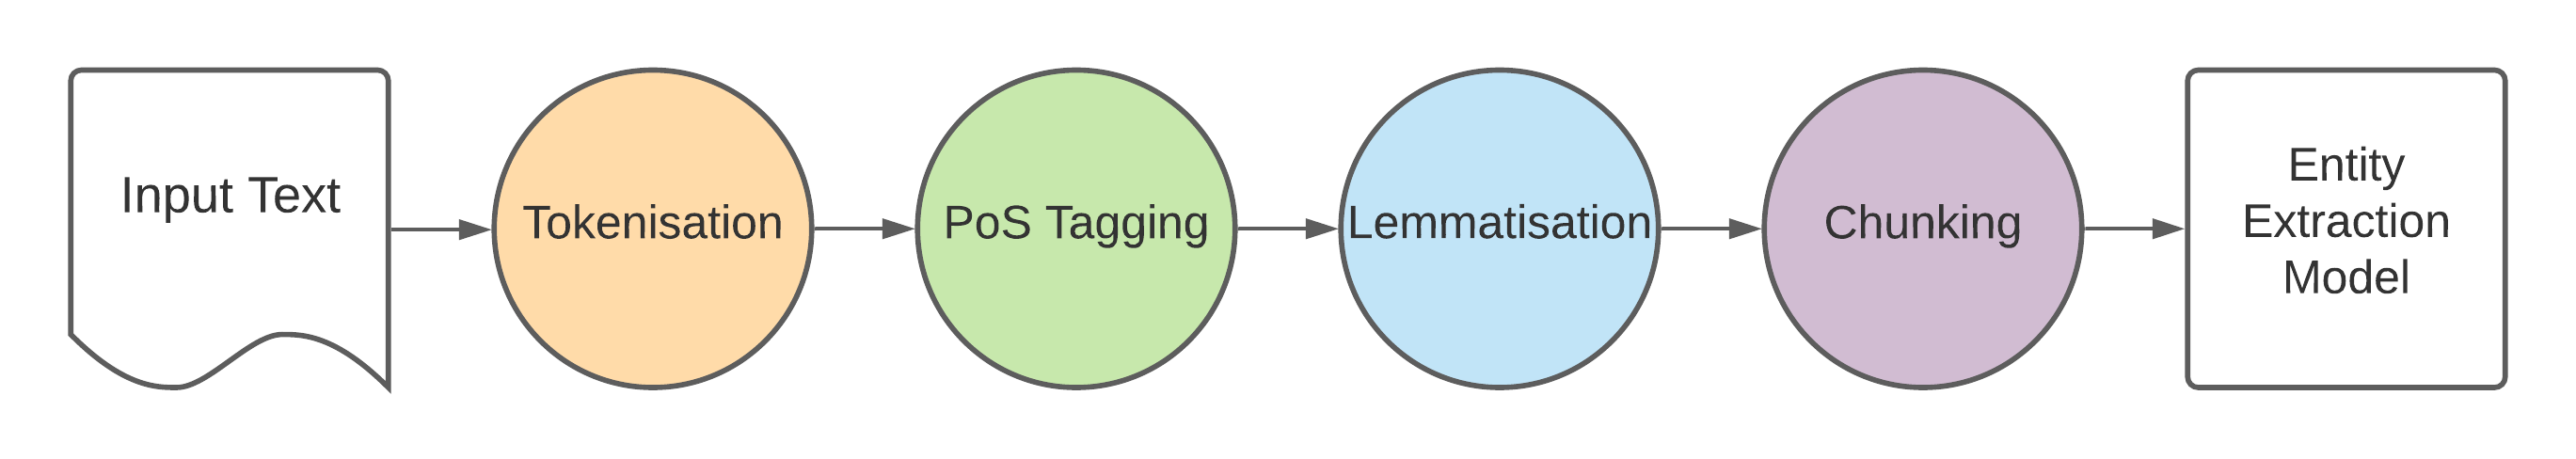
\includegraphics[scale=0.15]{images/sentence chaining}
\caption{Data preprocessing pipeline}
\end{figure}

\subsection{Tokenisation}
Tokenisation (as seen in \Cref{fig:tokenisation+pos}) involves breaking down the sentence to retrieve fragments called `tokens' which are pre-defined elements. These can include words, keywords, phrases, or symbols/ punctuation depending on the application~\cite{kannan2014preprocessing}~\cite{ieee_named_entity}. Once the tokens are obtained, often some filtering methods, such as stopword removal, are applied to prune any unnecessary tokens using a pre-determined set of words (often called `stoplist'). This list of words is not fixed but often contains words such as `are', `this', `that' etc. which are generally not crucial for document classification approaches~\cite{kannan2014preprocessing}. The questions of whether stopwords should be removed and/or which stopwords to remove are often dependent on the data mining problem.  

\subsection{Part-of-Speech (POS) tagging}

Part-of-speech (POS) tagging, also known as grammatical tagging, assigns `parts-of-speech' to words in a text.  It uses word and grammar structure taking into account the context around words to determine their characteristics, for instance, identifying a word as a noun, verb, preposition etc~\cite{pos}. POS tagging often assumes some sort of tokenised text upon which it makes the grammatical tag classifications as seen in~\Cref{fig:tokenisation+pos}. In the figure, the tagger identifies `Emirates' and `Bitcoin' as `PROPN' (proper nouns), `airlines' and `payments' as `NOUN' and as `accept' as `VERB'. POS tagging is a critical component of many NLP systems. It provides linguistic information about the text and enables information extraction from text corpora in order to identify key entities and relationships. 
% The set of tags depends on the model used and can involve course and/or fine classification. 
The set of POS tags is shown in Appendix~\Cref{appendix:pos}

\begin{figure}[H]
\centering
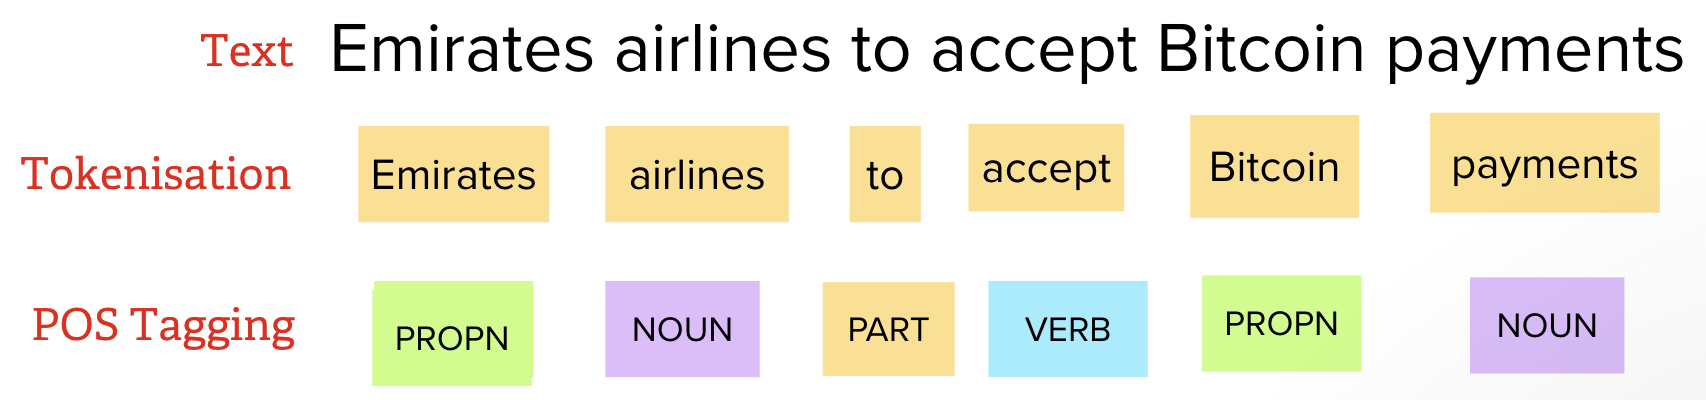
\includegraphics[scale=0.35]{images/token+pos.png}
\caption{Tokenisation and POS tagging}
\label{fig:tokenisation+pos}
\end{figure}

\subsection{Normalisation} \label{normalisation}

Information retrieval focuses on getting or providing users with easy access to the information they need. It does not only look for the right information but represents it in a manner that is easily understandable to users, stores the
information in an orderly manner and organises it in such a
way that it can be easily retrieved at a later time.

Normalising data is a key step in information extraction from the text. As the size of the data increases, it becomes especially important to represent data in a standard manner and reduce randomness~\cite{stemming}. There are two common methods of normalising data: 

\begin{enumerate}
    \item \textbf{Stemming} is the process of reducing words (or tokens) to their word stem or root form~\cite{stemming}. One of the most common algorithm for stemming English words is the Porter's algorithm. It makes use of a minimal length measure which is derived from the number of consonant-vowel-consonant strings that remains after a suffix is eliminated~\cite{porter}. The main drawback of stemming is that it relies on a crude heuristic process to condense related words into a single stem, even if it is not a dictionary word. This can result in errors caused by under-stemming or over-stemming~\cite{medium_stemming}. As an example of the latter, the words `participation' and `participate' may get reduced to `participat' which is not an actual word. 
    
    \item \textbf{Lemmatisation} is a form of normalising the data by matching words with their canonical (dictionary) forms called lemmas by reducing inflective variants to a `root' word/token~\cite{stemming}. Example: `walking', `walks', `walked' will all reduce to `walk'. Lemmatisation makes use of POS tags and sentence structure. This is a huge improvement over stemming as the base words are actual words and produces much better results for language modelling as described in~\cite{stemming}. 
    
\end{enumerate}

\subsection{Chunking}

Chunking is a process which essentially makes use of POS tags by attaching additional information to the sentence breaking it down into its constituent phrases. There are usually 5 major categories of extracting chunks from text: Noun Phrase (NP), Verb phrase (VP), Adjective phrase (ADJP), Adverb phrase (ADVP) and Prepositional phrase (PP). 
For example, the sentence ``The large truck is going under the tunnel" will be broken down into a noun phrase (NP): The large truck, verb phrase (VP): is going, prepositional phrase (PP): under the tunnel as in~\Cref{fig:chunking}.

\begin{figure}[H]
\centering

\includegraphics[scale=0.35]{images/chunking.png}
\caption{Sentence chunking}
\label{fig:chunking}
\end{figure}



\section{Dependency Parsing} \label{dependency_grammar}

Dependency parsing analyses the structure of a sentence based on word (token) dependencies. It uses a universal collection of tags, which is presented in Appendix~\Cref{appendix:deps}, to describe the relationship between two words, one acting as the `head' (parent) and the other as the `dependant' (child). A (token) word can have multiple dependents (one-to-many mapping) but can only have one head (one-to-one mapping). The `root' word of a sentence is one that is not the child of any other words in the sentence and is usually a verb and is often known as the `root verb'.

\begin{figure}[H]
    \centering
    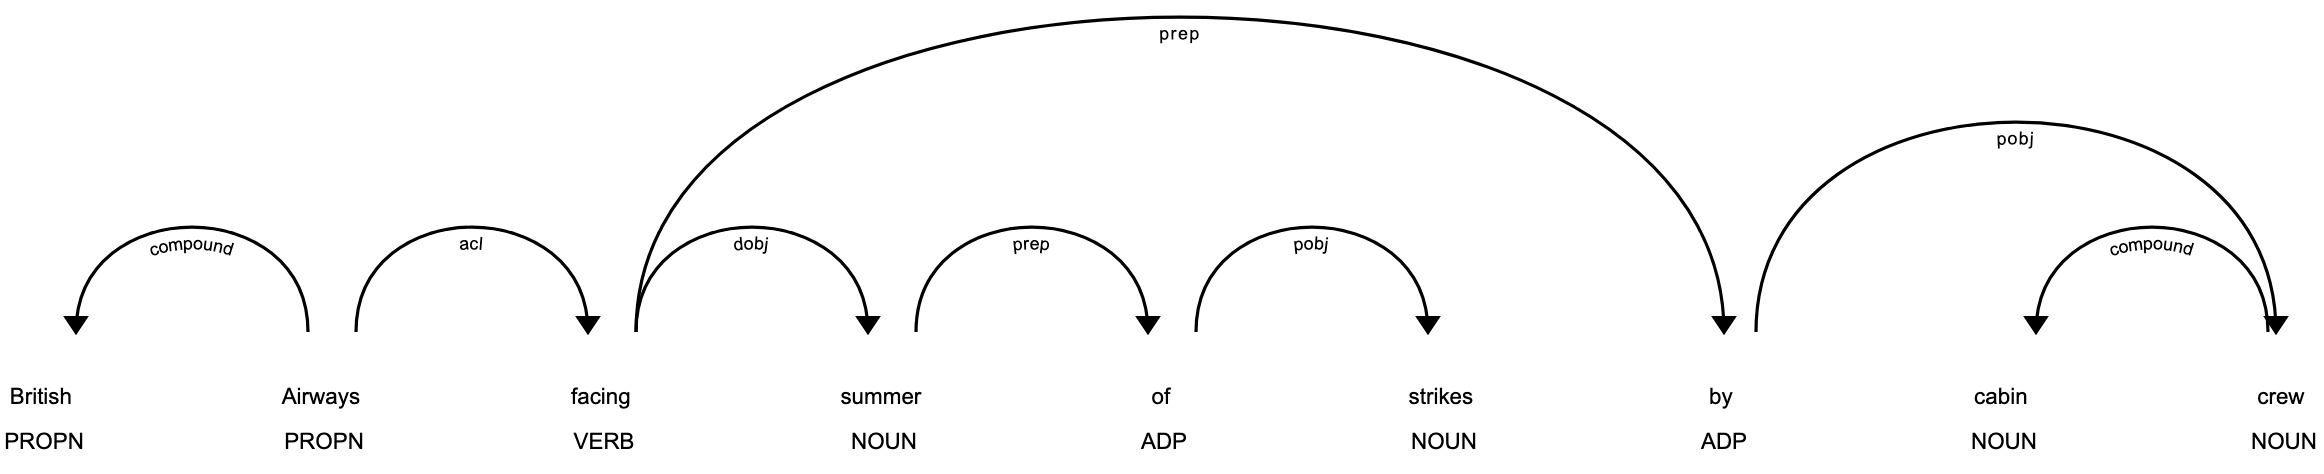
\includegraphics[width=\textwidth]{images/displayCy.png}
    \caption{SpaCy Dependency Tree Visualisation~\cite{spacy_ling}}
    \label{fig:displacy}
\end{figure}

\Cref{fig:displacy} illustrates the dependency relations and part-of-speech (POS) tags for each word (or `token') in the sentence. 

\begin{enumerate}
    \item `British Airways' and `cabin crew' are noun compounds, where all the nouns (e.g., `British') modify the rightmost noun (e.g., proper noun: `Airways').
    \item The noun `summer' is `direct object' of the `verb phrase' or predicate `facing'.
    \item Nouns `strikes' and `crew' are `objects of a preposition' or `pobj' as they are the `head' of noun phrases, `strikes' and `cabin crew' respectively, following adverbs or, in this case, adpositions (`of' and `by' respectively).

\end{enumerate}
 

\section{Coreference Resolution}

Coreference resolution refers to the task of ascertaining which linguistic expressions (known as mentions) in a natural language refer to the same real-world entity (such as a person or thing)~\cite{zheng2011coreference}. It is often an important step for other high-level tasks such as document summarisation and information extraction. The latter use case is particularly relevant to this project. When two or more expressions, refer to the same entity, they share the same referent~\cite{wiki_coref}. The goal of the coreference resolution algorithms is to find and cluster the mentions by their referent. For instance, in the sentence, ``The UK said they would relax travel bans'', the mentions `UK' and `they' refer to the same entity: `UK'

Coreference resolution is not a trivial task as it relies on both the semantic and syntactic meaning of the text. For example, in the sentence, ``Alice said she would come'', the mention `she' may or may not refer to Alice.  This indicates the complexity of the coreference resolution task as it requires contextual information, real-world knowledge, a grammatical understanding of the language etc.~\cite{zheng2011coreference}.

There are multiple different scenarios when exploring coreference. Some common ones include: 

\begin{enumerate}
    \item \textbf{Anaphora coreference: }
    Anaphoric references refer to the previous entities (the `antecedent') for their meaning. For instance, in this instance ``the aviation industry to find its way back in 2022", the anaphor `its' follows the expressions it refers to, the antecedent: `the aviation industry'. 
    
    \item \textbf{Cataphora coreference:}
    Cataphora references refer to entities/mentions that appear later in the text. For example, in the sentence, ``To aid their declining sales, Emirates is set to lower their fares", the cataphor `their' precedes the entity/expression it refers to, the postcedent: `Emirates'. 
    
    \item \textbf{Split antecedents/ Multiple Antecedent Coreference:}
    These references/words have multiple antecedents that they refer to. For instance: in the sentence ``British Airways and United Airlines set to resume their direct flights to Australia", the anaphor `they' has a split antecedent: `British Airways' and `United Airlines'. 
\end{enumerate}

\subsection{Span detection}

The primary step of coreference resolution is mention detection. This involves finding the `spans' i.e., the combination of words that constitute a mention. Generally, candidate spans cover NP (noun parts of the text), possessive pronouns and named entities~\cite{stanfordcoref} (discussed in detail in~\Cref{named_ents}). In order to detect spans, there are several options for span ranking architecture. Most models are more liberal in detecting candidate spans at the initial stages and then apply some filtering and/or augmenting mechanisms to get the most relevant spans. This can involve pruning candidate spans based on a threshold ranking score, considering only (pre-determined) K antecedents for each mention~\cite{lee2018coursetofine} or applying the span-ranking to the text in an iterative manner to update the span representations using prior antecedent distributions to allow later coreferences to be influenced by earlier ones \cite{lee2018coursetofine}. 


\subsection{Coreference Architecture}
Once the candidate spans are extracted from the text, the next step is to resolve coreferences of mentions. The most widely used architectures are as follows: 

\subsubsection{Mention-pair architecture} 
This is one of the simplest approaches and involves a binary classification task on a pair of mentions and/or entities. The classifier is given a pair of mentions, a candidate antecedent and a candidate anaphor and decides whether they are coreferring based on a ranking score. 

\subsubsection{Mention ranking architecture}

This type of architecture directly compares the candidate antecedents with each other,  selecting the antecedent with the highest score for each anaphor. This approach is more complicated than the mention-pair model as for each anaphor, the best possible `gold' antecedent is not known rather a cluster of `gold' antecedents is known. In earlier models, the `gold' antecedent was chosen to be the closest one. 

Generally, the simplest approach to give credit to any `legal' antecedent is by adding them together and using a loss function that optimises the likelihood of all correct antecedents in the `gold' cluster of antecedents~\cite{stanfordcoref}. This approach is used by the model in described in Lee 2017~\cite{lee2017end}, a model on many recent state-of-the art models such as SpanBERT~\cite{spanBERT} are based on. It uses the mention ranking architecture to determine a conditional probability distribution (as seen in \cref{cond}) to give a configuration with the highest likelihood representing the correct clustering. 

\begin{align}
 P(y_1, ..., y_n | D)  &= \prod_{i=1}^{N} P(y_i | D) \label[equationX]{cond} &\\
 P(y_i) &= \frac{\exp(s(x_i, y_i))}{\sum_{y' \in Y(i)} \exp(s(x_i,y'))}  \label[equationX]{coref_eq} &\\
\mathit{where} \ s(x_i,y')  &= s_m (x_i) +  s_m (y_i)  +  s_cf(x_i, y_i) \nonumber
\end{align}

In equation \cref{coref_eq}, goal of the task is to assign an antecedent to each span $x_i$ in document D. \( s(i,j)\) is a pairwise score which depends on three factors:  \(s_m(i)\), how likely span $x$ is to be a mention; \(s_m(j)\), how likely span $y$ is a mention and \(s_cf(i, j)\), the joint coreference probability of spans $i$ and $j$  in document $D$ (assuming they are both mentions) referring to the same entity \cite{lee2017end}\cite{lee2018coursetofine}.

\section{Word Representation}

The general idea behind word representation is to convert the text into an understandable format for the computer. This is done by word embedding which learns a vector representation for words.

\subsection{Types of embeddings} \label{types_embeddings}

There are several different approaches used for encoding words: 

\begin{enumerate}
    \item \textbf{Bag-of-Words (BOW):} The simplest approach for word encoding is the Bag-Of-Words approach where the general concept is to generate a dictionary of tokens from the text (say, news articles) by pre-processing the text using techniques such as stopword removal, lemmatisation and Named Entity Detection (NER) and then represent the documents/ news articles as a vector of the occurrences of those tokens in the text. In other words, the $j_{th}$ element in the vector (say 5) represents the fact that the $j_{th}$ token in the dictionary (say `London') appeared 5 times. This method is fairly primitive as it does not account for any grammatical rules and is an unordered representation. It falls short with increasingly high volumes of data as it is simply a syntactic representation and does not account for any semantic/ conceptual relations within the text corpus~\cite{elmo_word_rep}.
    

    \item \textbf{Term-Frequency-Inverse Document Frequency (TF-IDF):}  TF-IDF is a numerical statistic that indicates the significance of a word in a corpus (collection of documents). It is frequently used as a weighting factor in conjunction with the bag-of-words approach to represent document embeddings. The TF-IDF value is proportional to term frequency (TF) which represents the number of times a word appears in the document and is countered by the number of documents in the corpus that contain this word (IDF), thereby compensating for the fact that some words appear more frequently in general, and their high frequency is not distinct to a document~\cite{tfidf_mining}.
    
    \item \textbf{Word2Vec:} Word2Vec algorithms provide a much better way of word representation (or embedding) by using the concept of similarity of words. The core idea is that words that are syntactically and semantically close should have similar vector representations and thereby occupy similar spatial positions. This degree of similarity is calculated using the cosine similarity (cosine of the angle between two vectors)~\cite{efficient_word_rep}. They also exploit the `locality hypothesis' which centres around the notion that words that appear together or are close to identical  will be spatially close~\cite{elmo_word_rep}.

For simplicity's sake, let's say the word `know' is represented by a 4-dimensional binary vector [\_,\_,1,\_], with 1 in the third dimension then vectors for words that are variants of the same underlying root word such as `knew', `known' etc. will also have 1 in the third dimension, and those are not (say, `Monday') will not. Similarly, there can be a feature (dimension) (say, the $4_{th}$ dimension) representing a word type or category such as airlines and so, for instance, `Emirates', `Etihad' and `British Airways' should also have similar vector representations with the $4_{th}$ dimension (feature) having a value of 1, thereby assigning them to the same group (cluster)~\cite{32_contextual_word}.

These Word2Vec embeddings are commonly used in the Neural Network models: Continuous Skip-Gram and Continuous Bag-of-Words (CBoW)~\cite{efficient_word_rep}.

\item \textbf{GloVe:} Another popular approach is using GloVe or Global Vectors for word representation. Unlike word2vec which leverages co-occurrence of neighbouring words within a local context, the GloVe unsupervised model focuses on global statistics of word co-occurrences over the whole corpus. Like word2vec, it also relies on the mapping words in vector subspaces using semantic similarity of words \cite{glove}. 

\item \textbf{Context2Vec:} An improvement over Word2Vec is Context2Vec. This accounts for polysemy, the fact that in different contexts, words can have different meanings (or senses). This allows for a context-independent representation of a word, called ``contextual word vectors" which encapsulate the meaning of a word in a particular context. For instance, in the context of the sentence ``I ate a banana split", `split', is associated with food~\cite{32_contextual_word} and in ``the ice cracked and split'', `split' is a verb indicating breakage of ice.

This approach makes use of a bi-directional (left-to-right and right-to-left) LSTM (long short-term memory) recurring neural network. This network makes use of N layers of LSTM, where the lower levels extract low-level features such as POS tagging and the upper levels learn the contextual meaning of words ~\cite{elmo_word_rep}. One of the most popular approaches for this is ELMo (Embeddings from Language Models) which is discussed in \Cref{elmo}.
\end{enumerate}

\subsection{Embeddings from Language Models (ELMo)} \label{elmo}
\vspace{-4ex}

\begin{figure}[H]
\centering
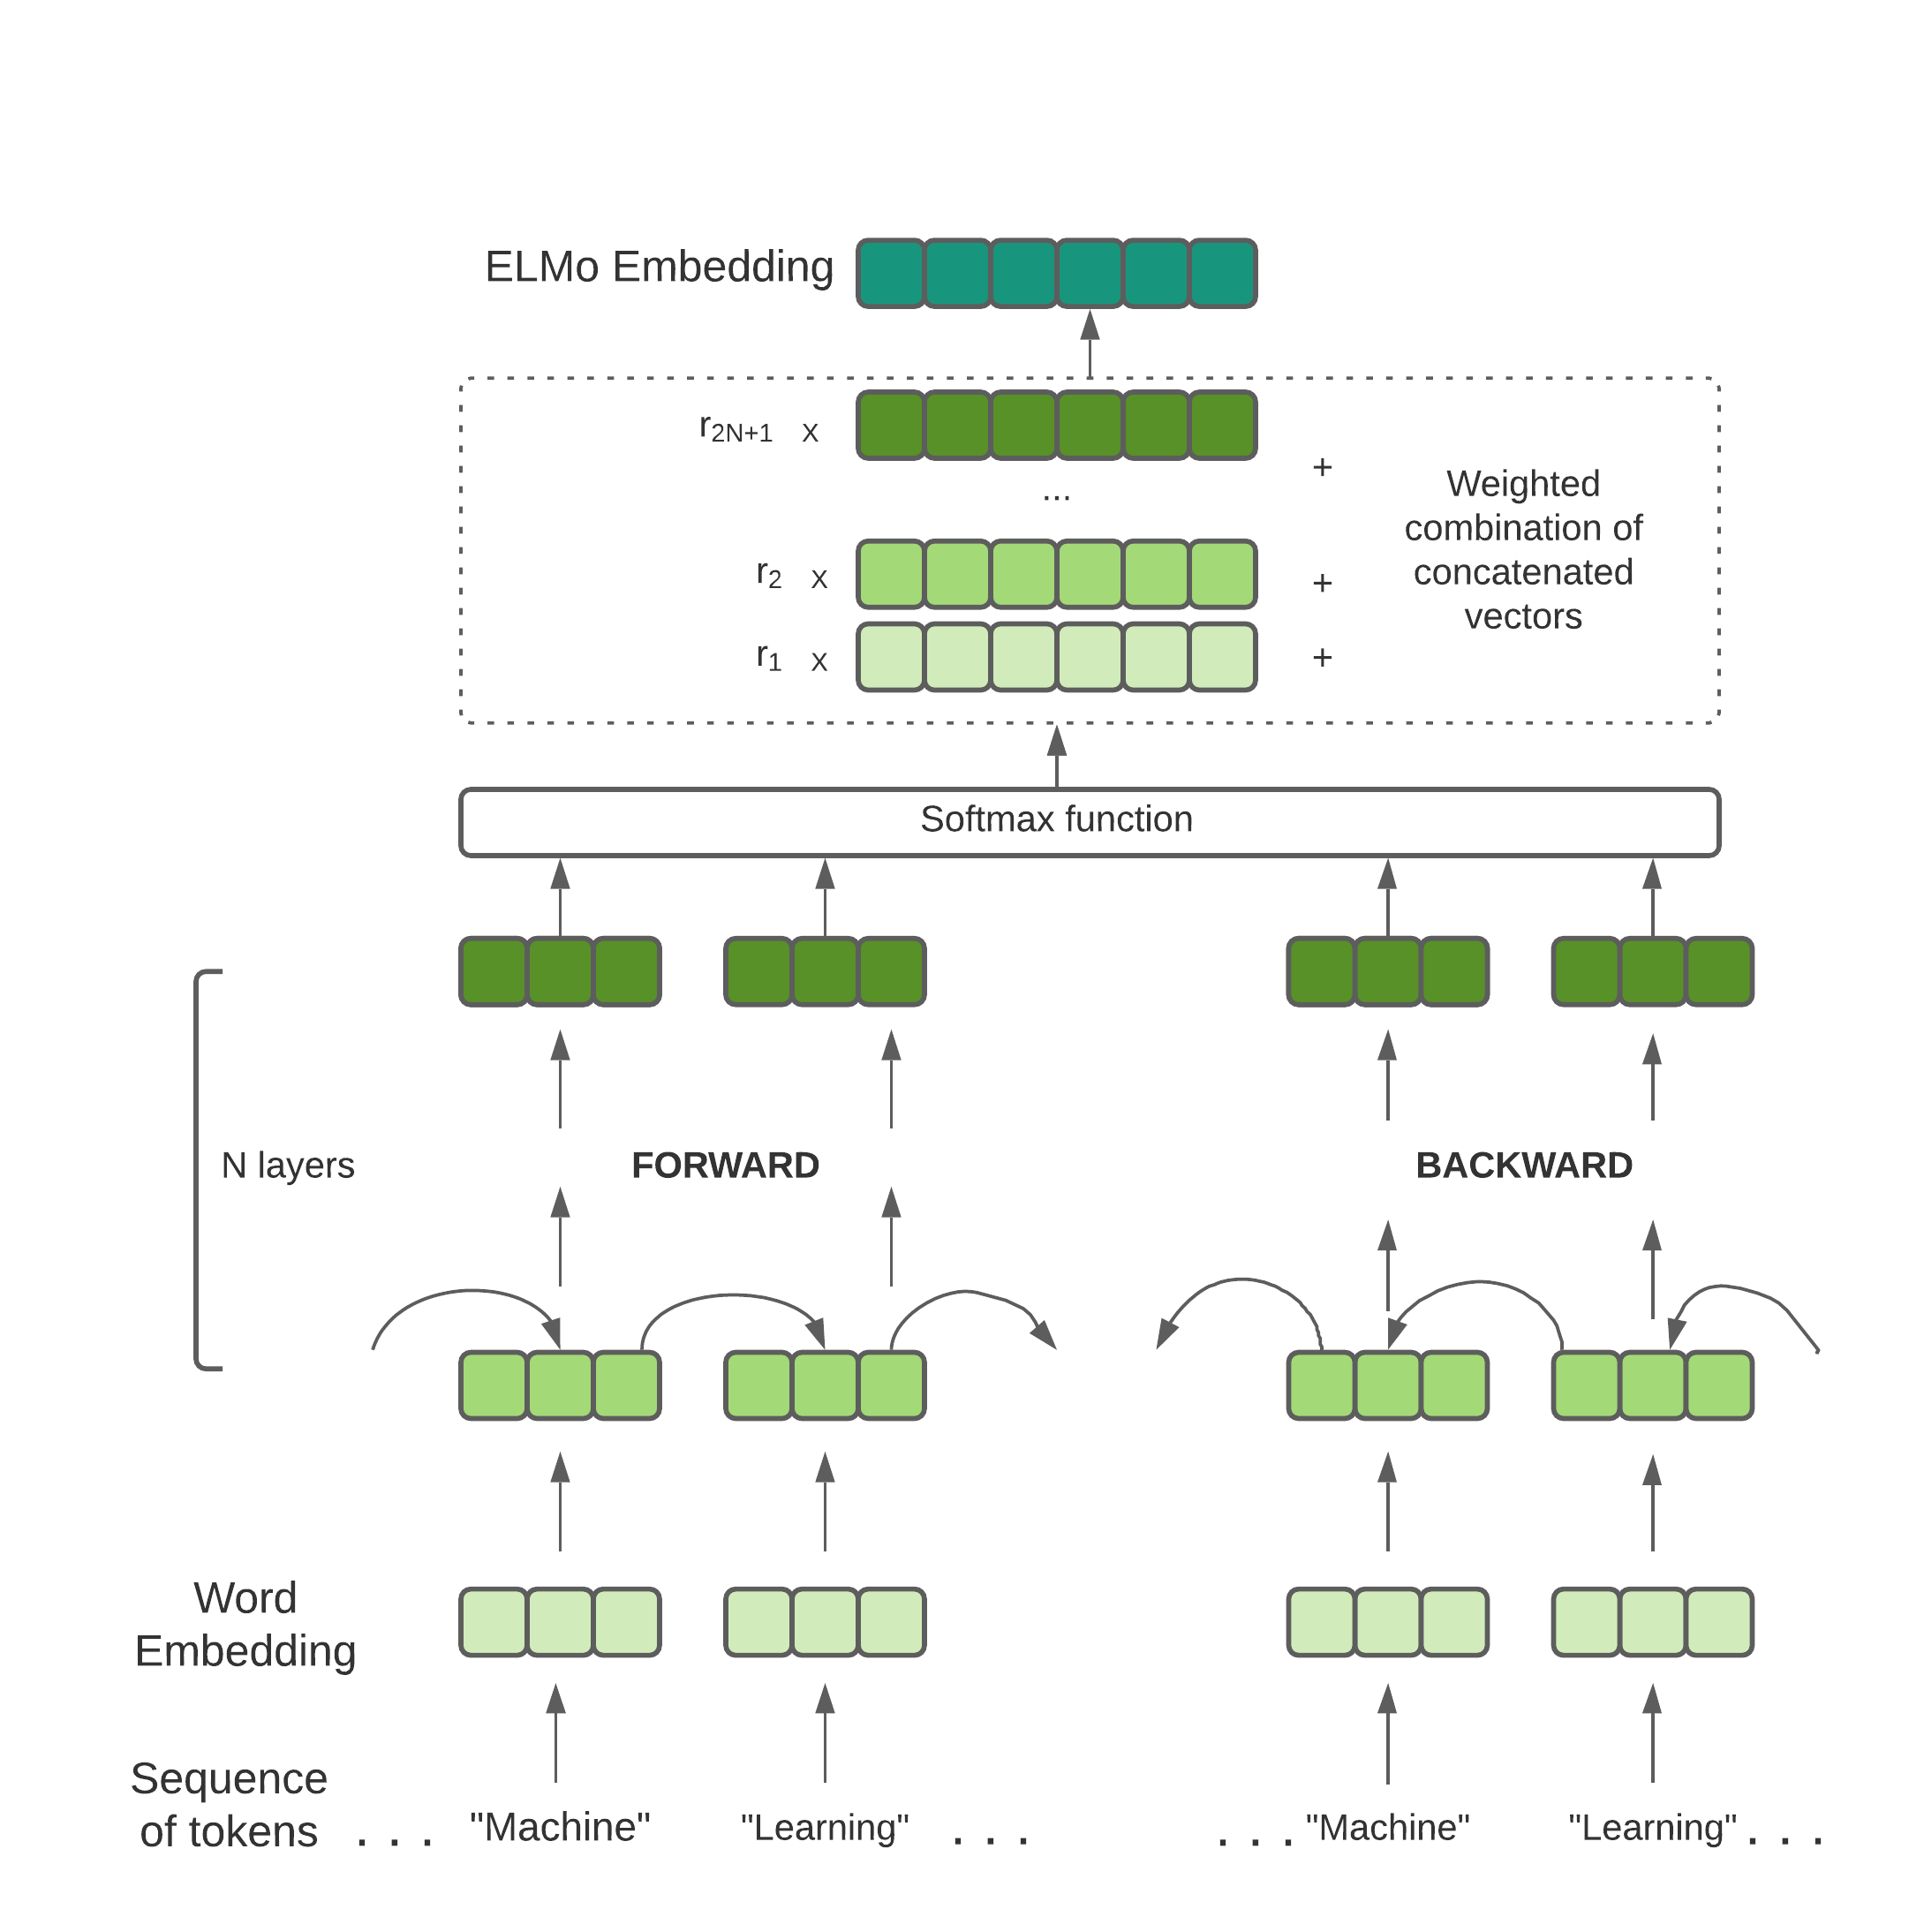
\includegraphics[scale=0.15]{images/Elmo2.png}
\caption{Embeddings from Language Models (ELMo) Context Representation}
\end{figure}


The outline of the ELMo model is as follows:~\cite{context2vec}

\begin{enumerate}
    \item The network consists of N bi-directional (left-to-right and right-to-left) LSTM layers and the input is  a sequence of N words/ tokens. 
    
    \item The Forward language model gets a sequence of words/ tokens (of arbitrary length) from left to right and calculates the probability of the sequence of words  $P(w_1, w_2, ... w_N)$ by making use of the history of words/tokens it has seen earlier~\cite{elmo_word_rep}.
        \begin{center}
            $P(w_1, w_2, ... w_N) = \prod_{i = 1}^{N} P (w_i | w_{1}, w_{2}, w_{i-1})$ 
        \end{center}
        
        For a target word/token $w_i$, let the context-dependent vector from this (forward) language model (at layer l = 1..N) be represented as LRV(i, l), which contains information about this word given the context of words appearing before the target word~\cite{elmo_word_rep}.
        
     \item Similarly, the backward model computes the probability of the reverse sequence of words as follows:
        
        \begin{center}
            $P(w_1, w_2, ... w_N) = \prod_{i = 1}^{N} P (w_i | w_{i+1}, w_{i+2}, w_N)$
        \end{center}
        
        For a target word/token $w_i$, let the context-dependent vector from this (backward) language model (at layer l = 1..N) be represented as RLV(i, l), which contains information about this word given the context of words appearing after the target word~\cite{elmo_word_rep}.
        
        \item The outputs from these models are passed to the subsequent layer of their respective models. A non-linear activation function (for example, ReLU) can be applied for intermediate layers. Softmax is applied to the outputs from the last LSTM layers of the 2 models~\cite{context2vec}.
    
        \item The objective function is to jointly maximise the log-likelihood in both forward and backward directions.
        
        \item For each word $w_i$, a N-layer biLM model will have a total of 2N+1 (including the input sequence of tokens layer) vector representations. The final vector (ELMo) which will be passed to the NLP training model, will combine these 2L+1 vectors by using a weighted sum of these vectors as seen in Figure 3. This is the ELMo embedding~\cite{elmo_word_rep}.
    
\end{enumerate}
% \section{Named Entity Extraction} 

% Extracting named entities from texts and representing them as nodes in knowledge graphs generally, involves three main
% tasks: Named Entity Recognition (NER), Named Entity Disambiguation (NED) and Named Entity Linking (NEL). 

\section{Named Entity Recognition (NER)} \label{named_ents}

Named entity recognition (NER) is a process which extracts and classifies named entities of certain (pre-defined) types such as `PER' (person), `GPE' (geo-political entities), `ORG' (organisation) from an unstructured text~\cite{ieee_named_entity}Refer to Appendix~\Cref{appendix:semantic_types} for the full list of entity types used by AllenNLP and spaCy. 

First, it identifies the `names' of the entities from the pre-processed tokens commonly done by BILOU tagging (See~\Cref{bilou}) and POS tagging. It then performs sequence labelling (assigning labels/tags to each element of an input sequence) and classifies entities into the predefined types such person, location, organisation and so on~\cite{ieee_named_entity}. \Cref{fig:bilou} highlights how the Named Entity Recognition process uses BILOU scheme to extract a ORG `Imperial College London' and GPE: `London'.

\begin{table}[H]
    \centering 
    \renewcommand{\arraystretch}{1.1}
    \begin{tabularx}{0.7\textwidth}{|>{\hsize=.1\hsize\linewidth=\hsize}X|>{\hsize=.2\hsize\linewidth=\hsize}X|>{\hsize=.6\hsize\linewidth=\hsize}X|} 
    \hline
    \textbf{Tag} & \textbf{Meaning} &\textbf{Description}  \\
    \hline
    \textbf{B} & Beginning & First token of a multi-token entity\\
    \textbf{I}  & Inside & An inner token of a multi-token entity\\
     \textbf{L}  & Last & Final token of a multi-token entity\\
     \textbf{O}  & Outside & A single-token entity\\
     \textbf{U} & Unit & A non-entity token\\
     \hline
    \end{tabularx}
\caption{BILOU tagging scheme}
\label{bilou}
\end{table}

\begin{figure}[H]
    \centering
    
\includegraphics[scale=0.35]{images/bilou.png}
    \caption{NER using BILOU}
    \label{fig:bilou}
    \end{figure}

\subsubsection*{Conditional Random Fields}
A popular sequence labelling model is \textbf{Conditional Random Fields }(CRF). These are ``discriminative models" and generally outperform other Markov Models and such as Hidden Markov Models (HMM) as they are better able to cope with unseen tokens/words as well as Maximum Entropy Markov Models (MEMM) as they do not have labelling bias~\cite{crf}.

They work by maximising the log-likelihood of the posterior distribution $P(s|o)$ where $s$ is the output label sequence and $o$ is the observed input sequence. Let $s'$ denote the correct label sequence: 

\[ s' = \argmax_{s} P (s|p) \]

Therefore, it is fairly simple to determine output label sequence as it will be the one with the highest posterior probability. E.g., P([PER, ORG, ORG] | [Obama, UN, Congress]) will have a much higher probability than  P([LOC, LOC, LOC] | [Obama, UN, Congress])~\cite{crf}, where `PER', `LOC', `ORG' refers to person, location and organisation respectively.

The NER models are usually trained on specific domains and thereby only extract certain pre-defined types of entities such as PER, LOC, ORG etc. (See Appendix~\Cref{appendix:semantic_types}), thereby making them domain-dependent.

% \subsection{NER Approaches}

% \begin{enumerate}
%     \item \textbf{Rule $/$ knowledge-based approaches:} These methods depend on pre-defined (hand-crafted rules). The primary advantage is the lack of need for annotated training data as they focus on lexical representation and resources. These can be useful for domain-specific uses as they are rules are exhaustive and can help extract model-specific knowledge, resulting in high precision model. A drawback, however, is they will perform poorly when extended to other domains, and poor generalisability means constructing and maintaining lexicon resources for many domains is costly.

%     \item \textbf{Learning-based approaches:} These methods replace the human-curated rules. These methods can be further classed
% into three types: supervised, semi-supervised, and unsupervised. Supervised and semi-supervised methods,
% require the ML model to be trained on the input input given the corresponding output data to learn the features mapping the inputs to the outputs. Common examples to model the classifiers include  Hidden Markov Models (HMM), Support Vector Machines (SVM), and
% Conditional Random Fields (CRF). The type of classifier can have an effect on the accuracy of the NER task. For instance, SVM and HMM do not consider the dependencies among words. The unsupervised,
% bootstrapped methods are generally more automated in that they do not require an expansive training set (seeds) and but are less common. 
% (seeds). \hyperlink{9}{[9]}

% \item \textbf{Feature-inferring neural-network approaches:} Like learning-based approaches they incorporate machine learning techniques, however, they automatically infer the features by using deep neural networks (DNNs) such as LSTM. Reportedly, \hyperlink{9}{[9]}, they generally outperform the other approaches. They are able to perform feature extraction in the lower layers of the network and use these to train the classifier. The advantage is that they do not require seeds, ontologies or any domain-specific lexicons and are therefore domain-independent making them more robust. However, they do require huge datasets to build a decent model.  \hyperlink{9}{[9]}
% \end{enumerate}

\subsection{Named Entity Disambiguation and Linking} \label{ned}

\textbf{Named Entity Disambiguation (NED)}: NER might not always be able to classify a named identity due to it having a different meaning in different contexts. This is why named entity disambiguation is crucial to determine which
named entity a mention refers to; For instance, `Trump' can refer to either a person, a corporation or a building~\cite{ieee_named_entity}.

A common approach for disambiguating entities is to use context representation using the entirety of the text to find co-occurrence of `entity mentions' to establish `candidate' entities and use an existing knowledge base through `Named Entity Linking' to learn about the entities. The information from the knowledge can be used in conjunction with candidate-entity ranking approaches can be used which involve ranking candidate entries and retrieving the one with the highest probability for a target mention. 
An example in~\cite{ned}(p.7) shows that for the sentence: ``Michael Bloomberg is the mayor of New York", their algorithm correctly identifies New York in USA instead of London as `Michael Bloomberg' co-occurs in the same paragraph as `New York' (in USA) ``(88 times) more than with the New York in England (0 times)'' in the knowledge base. Quantifying  the impact of co-occurrences, can be done by using incidence matrix represents a weighted graph where weights are the co-occurrence $|$P(e$_{i}$,s,e$_{j}$,t)$|$ i.e. count of paragraphs, where two different entities e$_{i}$ and e$_{j}$ were mentioned together in two different sentence forms (s $\neq$ t)~\cite{ned}. 

Additionally, \textbf{Named Entity Linking (NEL)} uses a standard (unique) International Resource Identifier (IRI)~\cite{internationalized} for each disambiguated entity as described in a Knowledge Base (say, Linked Open Data (LOD) Cloud). Entity mentions are annotated by some NER algorithms, but they are restricted to the pre-defined types (such as persons, locations, organizations)~\cite{ieee_named_entity}. Knowledge base (KB) hosts millions of entities and therefore NEL can be used to ground mentions of entities in some text to a central KB. An example mentioned in~\cite{nel} highlights this: ``David Murray recruited from Positive Black Soul'' grounds Wikipedia articles for `David Murray' (saxophonist) but not the `David Murray' (musician) (disambiguation based on context). 
    
% \end{enumerate}

% \subsection{Named Entity Linking (NEL)}

% \textbf{Named Entity Linking (NEL)} aims to provide a standard IRI for each disambiguated entity as described in a Knowledge Base (e.g. Linked Open Data (LOD) Cloud). Entity mentions are annotated by some NER algorithms, but they are restricted to the pre-defined types (such as persons, locations, organizations). \hyperlink{9}{[9]} Knowledge base hosts millions of entities and therefore NEL can be used to ground mentions of entities in some text to a central KB. An example mentioned in this \hyperlink{14}{paper [14]}  highlights this: 'David Murray recruited from Positive Black Soul' grounds Wikipedia articles for David Murray (saxophonist) but not the David Murray (musician) (disambiguation based on context) and Positive Black Soul. 

% NEL has three main sub-tasks:

% \begin{enumerate}
%     \item Candidate-entity generation: tries to extract all possible entities in the knowledge base (KB) that could potentially refer to an entity mention in the text. This can be done by dictionary-based approaches, supervised learning of surface (sentence) form expansion from documents or probability-based approaches. 
    
%     \item Candidate-entity ranking: this step resembles disambiguation as seen in NED. This involves ranking candidate entries and retrieving the one with the highest probability for a target mention. The ranking can be established  via supervised methods (which include graph-based, model ensemble and probabilistic approaches) as well as unsupervised methods (which include Vector-Spaced Model and Information Retrieval based approaches.) \hyperlink{9}{[9]}
    
%     \item NIL clustering: handles those mentions in the text that have no matches with any entities in the knowledge base (KB). Of the three steps, this one is often not developed extensively. This can be implemented using string matching (grouping entities based on the string),  graph-based approaches (use a semantic entity graph) and hierarchical agglomerative clustering (based on minimising a distance metric). \hyperlink{9}{[9]}


%     \end{enumerate}
    
    
% \begin{figure}[H]
% \centering
% 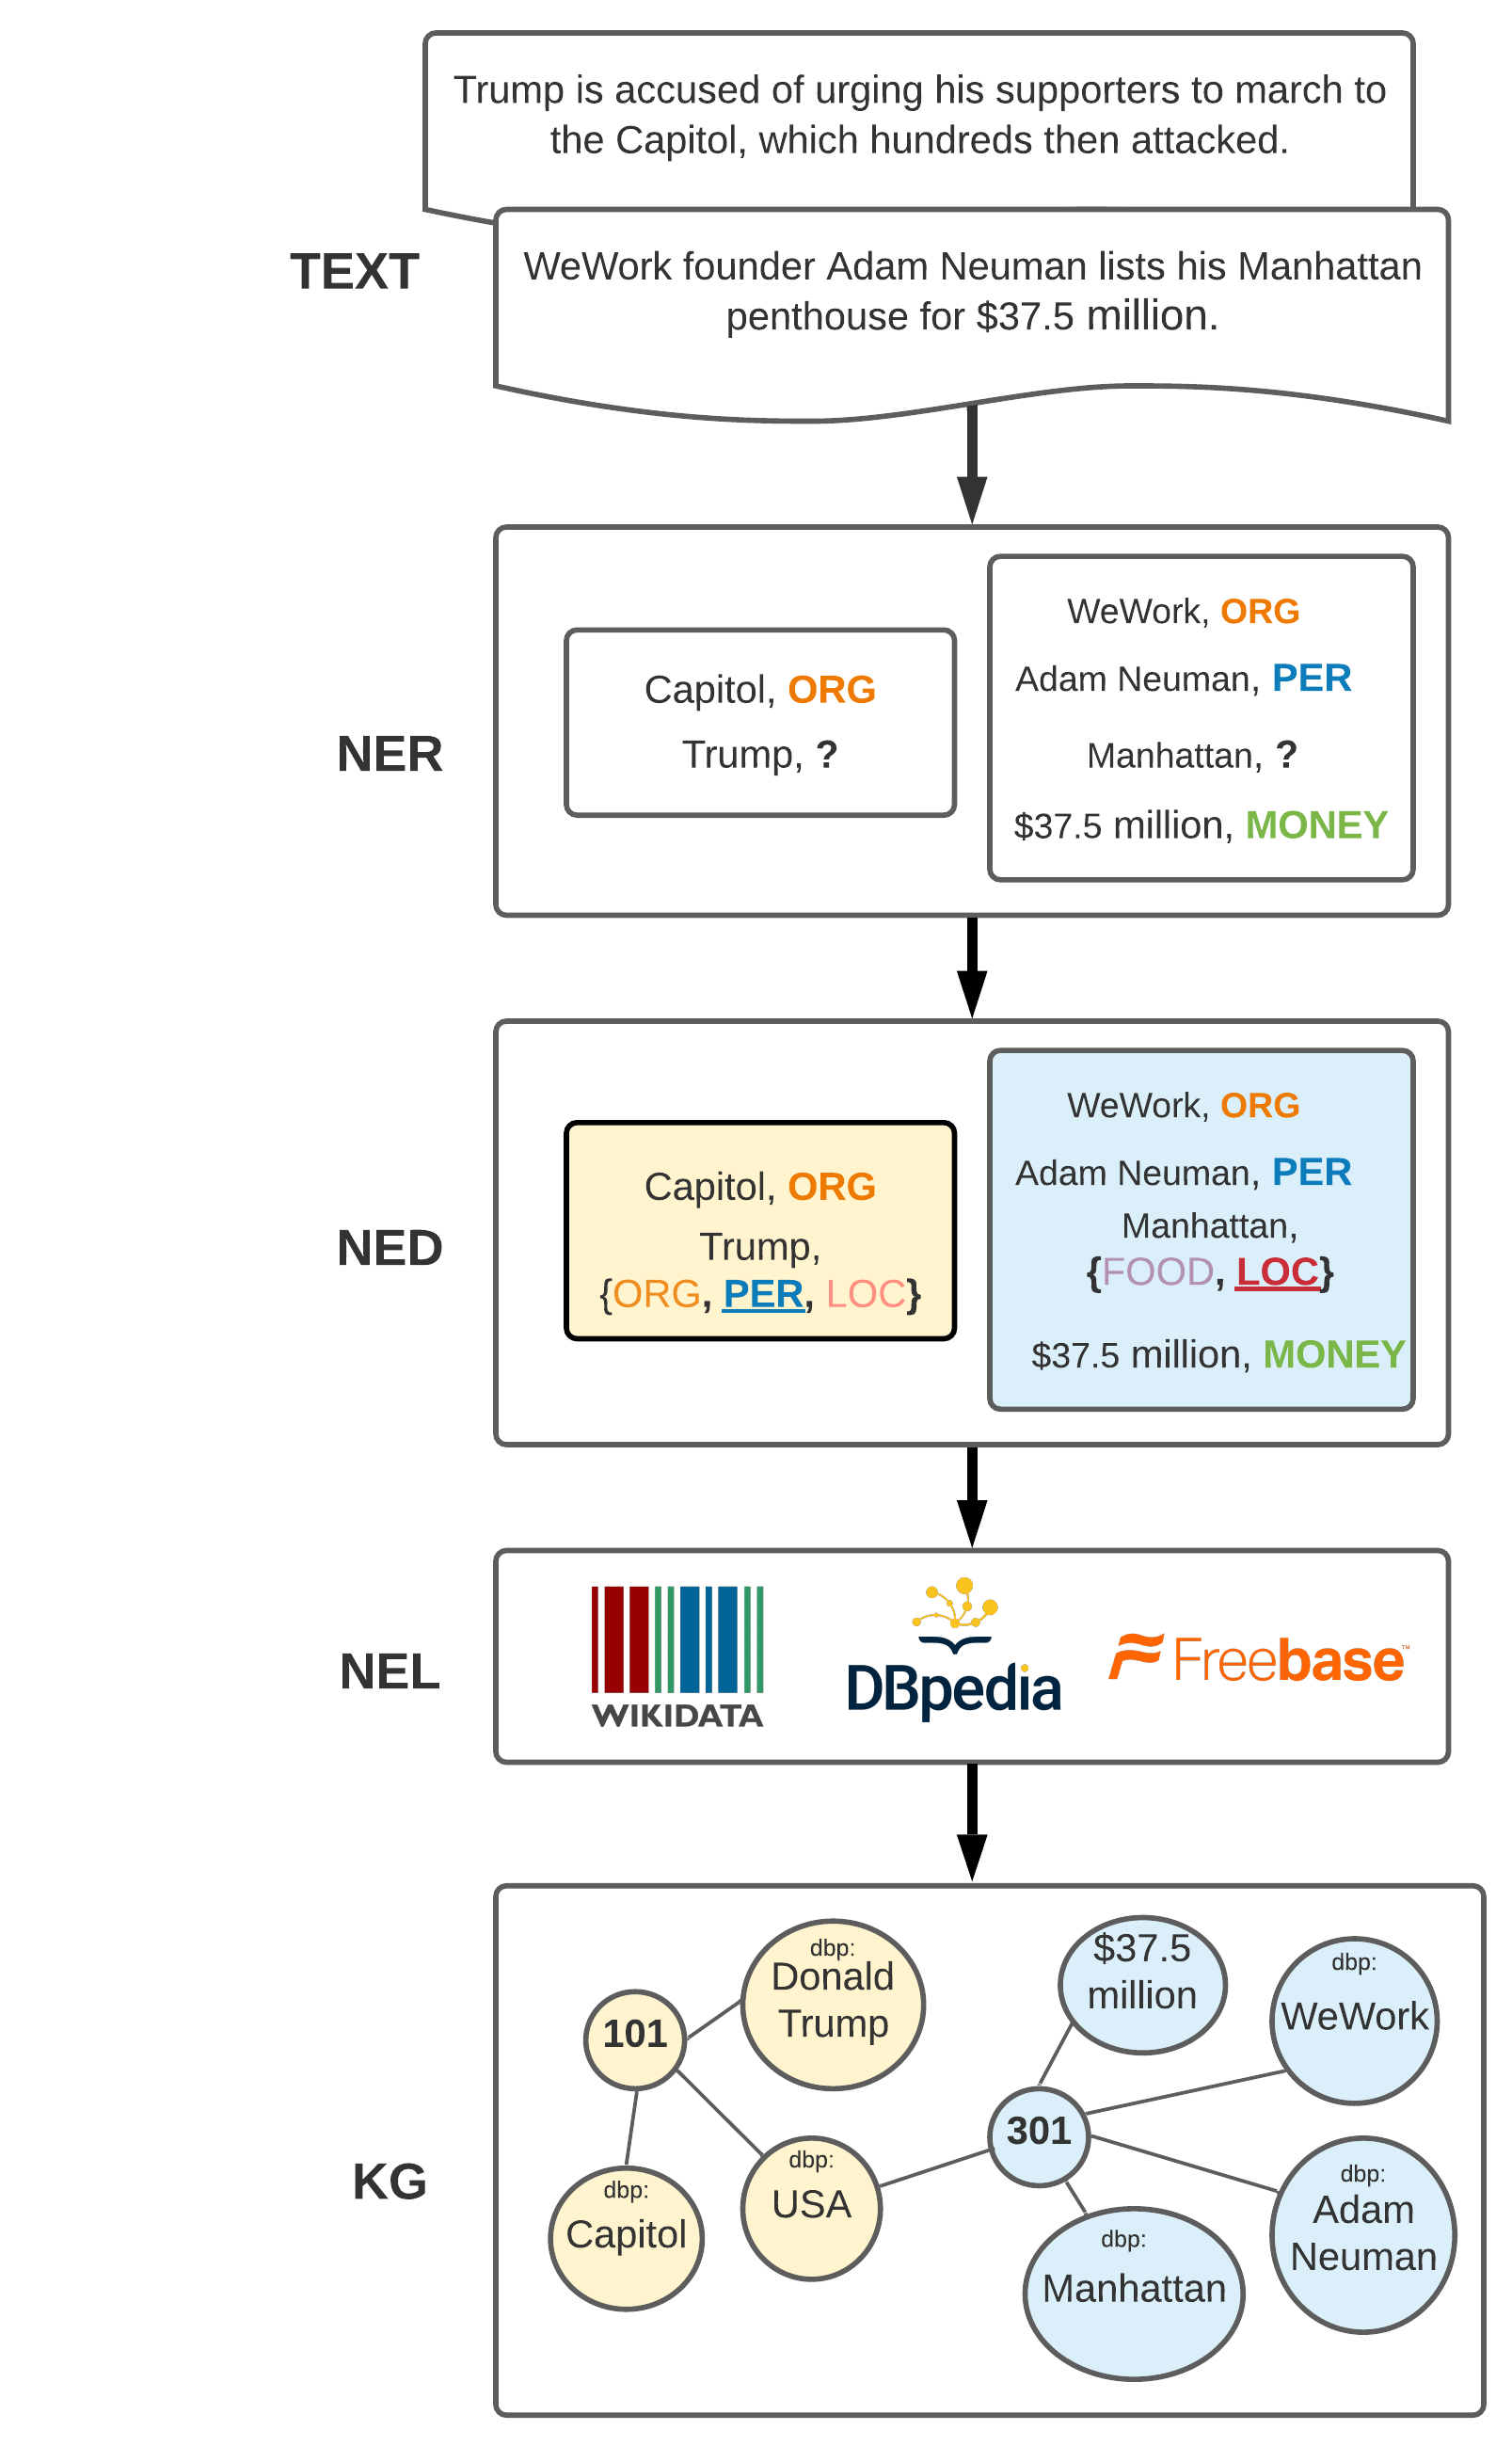
\includegraphics[scale = 0.2]{images/pipeline.png}
% \caption{Named Entity Extraction}
% \end{figure}
\section{Topic Modelling}

% https://reader.elsevier.com/reader/sd/pii/S0957417420310149?token=92A0D1D9A754D75A93CFCCCC73D7A93ED7D8A366D40B906DA60A1E44B3B2ADCB28B35A257530B241BF02F5D48485CD47&originRegion=eu-west-1&originCreation=20220123195220 
Topic modelling is essentially finding patterns in collections of data (in our case, news articles). The motivation behind topic modelling for this project would be to condense the key themes/ topics per industry from vast collections of news articles (grouped by industry). \hyperlink{24}{[24]}

% % https://journals.plos.org/plosone/article/file?id=10.1371/journal.pone.0064846&type=printable
Topic models are essentially based on Bayesian Networks and "assume that shared global multinomial word distributions (i.e., topic distributions) govern the corpus" \hyperlink{23}{[23](p.2)}.  Each of these documents (news articles) will contribute to the frequencies of a word in a document which is derived from a mixed model of the topic distributions.

\subsection{Main Approaches}

There are 2 main methods for topic modelling: 

\begin{enumerate}
    \item \textbf{Latent Semantic Indexing (LSA):} often implemented as pLSA (probabilistic Latent Semantic Indexing) works by creating a semantic space from large collections of text. This space is then used can then be used to detect similarity among words, topics, or even entire documents. This semantic space is a large high-dimensional vector and is essentially a term-document matrix (with columns representing documents and rows representing unique words/topics). To reduce the high dimensionality of the vector, often dimensionality reduction methods such as Singular Value Decomposition (SVD) or Principle Component Analysis (PCA) are used. A drawback of LSA is that it makes the orthogonality assumption that each document is about one thing which intuitively is not true for most documents. Another limitation is that these methods may require a way to interpret the high-dimension vector as it has minimal legibility value for humans. \hyperlink{24}{[24]} 
    
    \item \textbf{Latent Dirichlet Allocation (LDA):} The other much more popular model is LDA. It is a hierarchical Bayesian model, where each document is modelled as a mixture (multinomial distribution) of topics with each topic itself being a mixture of (multinomial distribution) of words.  \hyperlink{25}{[25]}. It is important to note that each topic can have multiple words, every word in the text corpus is tagged with a single topic. This essentially means that a word's presence can be attributed to one topic's distribution (even though in reality it could be present in the text corpus as a result of multiple topics). 
    
    Additionally, LDA ensures sparsity in the underlying multinomial distributions by making use of the Dirichlet prior distribution. This aids in the interpretations of the extracted topics. \hyperlink{23}{[23]}
    
    In order to extract the key topics within a volume of data (for the scope of this project, news), some sort of metric is needed to extract the relevance of a topic.   
One such approach is highlighted in this \hyperlink{23}{paper. [23](p.3)} 

It defines I$_{k}$ (t), the news on a day t associated with a topic k as the  "total numbers of words tagged with topic k on day t". 

\begin{center}
    $ I_{k} (t) = \sum_{I(t)} \sum_{w} N (d, w, k) $
\end{center}

where N(d,w,k) represents the frequency of word w (tagged with topic k) in the document d. I(t) is the represents the documents/ news articles obtained on day t. Equation cited from \hyperlink{23}{paper. [23](p.3)} The topics for which $I_{k} (t)$ returns the largest values can be thought of as 'most relevant' for that day. Additionally, the relevance of a topic k over time can also be determined by computing this value for different days (changing t).

    
\end{enumerate}

\subsection{Considerations for Topic Modelling}

An issue that needs to be considered when extracting topics for large volumes of news articles is that majority of them might have repeated and unwanted phrases such as "Top News" or "Read Similar Articles" that may be extracted as topics even though they have no intuitive relation to the news pertaining to a specific industry. Eliminating these phrases may be computationally heaving and require extensive parsing, as well as require an algorithm that accounts for all variations of such phrases. Therefore, a better approach to avoid this as discussed in \hyperlink{23}{[23]} is to prune topics based on their distributions by focusing on top N (for instance, 6) words associated with a topic distribution and eliminate this topic if any of these N words are in a pre-defined dictionary of words derived from unwanted phrases.

Topics modelling can be used in conjunction with sentiment analysis, whereby a single joint model performs both i.e. extracts topics and sentiments. This idea stems from the notion that every opinion has an associated target (quadruple discussed in Section 2.4).  Based on concepts mentioned earlier, topics modelling can be used to extract aspects which can be topics or sentiments. However, there will be no differentiation between the two. To combat this, some sort of an indicator variable may be used to make that distinction. \hyperlink{16}{[16]}

% --------------------------------------------------------------------------------------------
\section{Sentiment Analysis}

Sentiment analysis is used to express whether a piece of text (can be about a 'target entity' in the text, topic in the text, a sentence or the whole document) implies a positive, negative or neutral sentiment. Sentiment analysis (or opinion mining) requires extracting the semantic orientation (polarity and strength) of the text. An example of this can be done by assigning a score in the range of [-1,1] where +1 can indicate an (extremely) positive sentiment and -1 can indicate an (extremely) negative sentiment with 0 being neutral. \hyperlink{16}{[16]} \hyperlink{18}{[18]}

It is important to understand the structure of the sentiment (or opinion). Using the definition in this \hyperlink{16}{book [16]}, an 'Opinion' represents a "\textit{quadruple (g, s, h, t) where g is the sentiment target, s is the sentiment of the opinion about the target g,
h is the opinion holder (the person or organization who holds the opinion), and t is the time when the opinion is expressed.}" Furthermore, g can be split into entity (e) and aspect of entity (a$_{i}$), where each entity can have multiple aspects and the sentiment is based on the aspects of entities and not the entities as a whole. This allows entities to have multi-faceted sentiments. \hyperlink{18}{[18]} 

The main steps of sentiment analysis involve: 
\begin{enumerate}
\item Pre-processing the raw text (e.g. news articles) to using techniques such as lemmatisation, Parts-of-Speech Tagging (POS) and Stop Word
Removal to break down each text document into its components (such as phrases, tokens etc.) \hyperlink{17}{[17]}
\item Identifying sentiment bearing phrases and assigning it a sentiment score, which can then be combined to assign a multi-layered sentiment.
\end{enumerate}

For this project, I will do sentiment analysis on each of the key entities in news (pertaining to specific industries.) Therefore, it may be useful to use the notion of subjectivity (strength) and polarity scores at global and entity levels as mentioned in this \hyperlink{22}{[paper. 22]} where world scores use "total references" (denominator) to mean all the references of the entity from a history of news articles (global level) not just those references extracted from processing the news on a single day (entity level).  

In the case of news articles, some of the automatic opinion mining systems can usually associate entities mentioned in the context of negative articles with a negative sentiment even if the entity may have acted positively. For Example, if an airline company was giving out free upgrades to those whose flight got cancelled without notice due to the pandemic, the airline might be associated with a negative sentiment due to the nature of the news (cancelled flights, pandemic) surrounding that airline even though they were being generous to their customers (which would warrant a positive sentiment). Therefore, often, when dealing with sentiment analysis, models consider windows of variable size surrounding these entities as discussed in this \hyperlink{20}{paper [20]} to gauge a better context of the entity for determining the sentiment associated with it.


\subsection{Sentiment Analysis Approaches}

Generally, there are two approaches to sentiment analysis: 

\textbf{1. Rule-based sentiment analysis}
These techniques are rules and dictionary-based. A sentiment reference dictionary that contains keywords phrases labelled by sentiment is used to classify the sentiment of the sentence/text. These scores require rules to ignore or account for sentences (or parts of a sentence) containing negations, dependent clauses or even sarcasm. The advantage of these methods is that they incur less  computation overhead as there is no training needed. However, their drawback is that they often lack context and do not consider semantic relationships thereby resulting in low accuracy. 

\textbf{2. Machine Learning (ML) based sentiment analysis}
These methods use a machine learning model to classify the sentiment based on words and their lexical ordering by using a labelled-training set (supervised approach). These methods are sensitive to the training data and need to account for class imbalance. This class imbalance can be dealt with by using ensemble methods such as random forests as highlighted in this \hyperlink{18}{paper. [18]}. The advantage with them is that they be customised to the domain.

\subsection{Considerations in scoring sentiment data}

The scoring metric can make of use of techniques like Adverb scoring axioms such as adverbs of degree (AoD) where for example, adverbs such as 'extremely', 'absolutely' and 'hardly' indicate the strength of the sentiment or  Adverb-Adjective combinations (AAC) scoring axioms such as Variable scoring, Adjective priority scoring (APS) as discussed in this \hyperlink{17}{paper. [17]}


Generally, it can be seen that phrases separated by 'and' have the same polarity and those separated by 'but' have reverse polarity. 

As mentioned before, it is essential to account for negation and modifiers when assigning the sentiment score, this can be done in an approach described in this paper \hyperlink{22}{[22]} where the polarity of a 'sentiment word' can be flipped if it is negated. For instance, if 'good' has a polarity of +1 , then 'not good' will have negative polarity of -1. Similarly, when accounting for modifier, the strength of the sentiment is altered, so for example, 'extremely good' can have a polarity strength of +2. 


Additionally, pronoun resolution can be incorporated as well to get more entity sentiment additional co-occurrence relationships between entity and sentiment compared to the original news article. There is also a need to consider a way to obtain co-reference sets that allow the resolution/aggregation of aliases of entities. E.g. Donald Trump and Donald J. Trump should refer to the same entity. \hyperlink{22}{[22]}

Another potential consideration is the use of duplicate news articles having an effect on the sentiment score. For this reason, the model should eliminate redundancy of articles by not considering those duplicated articles. \hyperlink{22}{[22]} 

\section{Visualising data}


% https://link.springer.com/content/pdf/10.1007%2F978-3-030-56146-8.pdf
%-----------------------------------------------------------------------------------------
\subsection{Data Preparation}
First and foremost, it is important to understand the goal of the visualisation, what precisely is needed to be visualised and think about what type of data is required for this. This data (news articles) can then be processed to transform and summarise it, extracting key pieces of information that is determined to be essential to the application. This transformed data/ information can then be stored in our desired format and utilised to output the visualisation. 

\subsection{Principals of Visualisation}

\begin{enumerate}
\item \textbf{Simple}
It is important to ensure that the visuals are simple and intuitive. The information that is most relevant to the application must be clearly and succinctly visible and organised in a consistent manner. Adding any unnecessary information can make the visualisation convoluted and difficult to understand. \hyperlink{29}{[29]}

\item \textbf{Standard}
Standardisation of data structure and elements is needed for a good visualisation. This requires handling any complexities and discrepancies in the data as well as eliminating redundancies. Examples of this include, but are not limited to, using common abbreviations, identical scaling, consistent layouts across your data visualizations. \hyperlink{29}{[29]} Additionally, it is important to provide context for these visualisations as well by using standardised labelling and indexing. \hyperlink{30}{[30]}

\item \textbf{Scalable}
Scalability, in this context, refers to the ability of a visualisation to adjust with the increasing volumes of data seamlessly. This increase should have minimal impact on the speed as well as the performance of the program. Additionally, this also relates how to fit the virtualisation by dynamically scaling it to the virtual space as it grows. \hyperlink{29}{[29]}

\item \textbf{Identify target audience}
 For the visualisation to be a good representation of the data, it is important to identify the target audience and how they will interact/ use the visual. As mentioned before, exploiting visual details like size, colour, position, font etc can allow for a more intuitive design whilst directing the focus of the users to key bits of information. \hyperlink{30}{[30]}

\item \textbf{Making use of interactivity}
It can be useful to leverage the interactivity in the visualisation, thereby allowing for a multi-faceted visualisation based on the context that the users choose. For example, if a user wants to the see key news related to the airline industry, the visualisation can zoom in to focus on the part of the visualisation specific to that sector. User interactions should be intuitive and simple so as to not confuse the user and discourage participation. 

\end{enumerate}


% \subsection{Future work: Self-Organising Maps}

% Self-organising maps (SOM), also known as Kohonen maps, is a type of neural network that uses unsupervised learning and aims to reduce continuous high multidimensional data onto discrete low dimensional by making use of a feature map and neighboured function based on some metric of similarity. They make use of topographic maps which follow the "principle of topographic map formation" where each new piece of information will be stored in its neighboured (derived from context). Additionally, neurons accessing related information will be stored nearby for quick interactions and updates. \hyperlink{26}{[26]} 

% The SOM algorithm consists of four key stages:\hyperlink{26}{[26]}\hyperlink{27}{[27]}

% \begin{enumerate}
%     \item \textbf{Initialization: }
%     This is where all the weights of neurons are initialised with small values that are randomly generated. 
    
%     \item \textbf{Competitive stage: }
%     In this stage, the algorithm picks the best matching or 'winning' neuron by computing a discriminant function. The competitive aspect arises from the fact that the neuron with the smallest value for this function is the 'winning' neuron. Euclidean distance is often picked as the discriminant function. Therefore, for an input vector v, the best matching neuron is the neuron whose weight is the smallest Euclidean distance away. This is generally referred to as Best Matching Unit (BMU). So, for neurons (n) and a randomly drawn input sample v, the BMU can be determined by: \hyperlink{27}{[27]}

%     \begin{center}
%          $ n_{BMU} = argmin_{n} \left\lVert w_{n} - v \right\rVert $
%     \end{center}


% \item Cooperative stage: 
%     This stage makes sure that the weights of the neurons in the same neighbourhood have an effect on each other and are not modified independently of one another. Once the winning neuron is established, the weight of this 'winning' neuron is updated. However, now similar updates to the weights of the neighbouring neurons must also be made. This requires a neighbourhood function that gets the topological neighbourhood of a neuron which is centred (symmetrical) around the winning neuron and decays with increasing (lateral) distance. This function $\Lambda$ can be defined as follows: 
%     \begin{center}
    
%         $\Lambda(i, j) = \frac{( \left\lVert r_{i} - r_{j} \right\rVert)^2}{2\sigma^2} $
        
%          \end{center}
         
%         where  i is the winning neuron and $\left\lVert r_{i} - r_{j} \right\rVert$ is the  lateral (lattice) distance of neuron j from the winning neuron and $\sigma$ is the standard deviation which decays exponentially with time. This is useful as this method is translation invariant. \hyperlink{26}{[26]}\hyperlink{27}{[27]}
        
        
% \item \textbf{Adaptive process: }
%         In order to get the features mapping the input space to the output space, a learning process is involved. This uses a learning parameter ($\alpha$) that decays over time (iterations/ epochs). From this, the weight rule can be defined as follows:
        
%         \begin{center}
    
%         $ w_{i} = \alpha (t) \Lambda (i, j, t) (v - w_{i})$
        
%          \end{center}
       
%       The weight updates will gradually move the winning neuron's (i) weight as well as its neighbouring neurons to be close to the input vector. The closer the neighbouring neuron j to the winning neuron, the greater the change to its weight. Over time/epochs, the radius of the neighbourhood decreases (so the number of neighbours decreases). This is done to promote the learning to have a significant effect on the weights (of neurons) during the initial/early iterations but not allow them to be  influenced by far away neurons in later stages of the training (encouraging convergence) \hyperlink{26}{[26]}
       
% \end{enumerate}


\chapter{Ethical Considerations}
\vspace{-2ex}
This project mainly focuses on mining news articles to visualise what can be interpreted as the key news and entities in an industry. From an intelligence standpoint, this could be extremely useful as it condenses large amounts of news to give a visual overview of an industry. Though this project might highlight recent developments and trends in a sector, it is extremely unlikely to influence and propagate some radicalised opinion. 

There is no direct human interaction in this project, neither does it require any collection or direct use of personal data. It should be mentioned that data will be used from large open-source knowledge graphs where there may be data regarding a person of interest that may be deemed personal. E.g. Person: Donald Trump, Location: White house. However, any data that is in public domain will not be considered private or sensitive. Wikidata releases all its data under Creative Commons CC0 (public domain). \hyperlink{35}{[35]} 

One important ethical consideration, however, is to think about any bias introduced in the model/ visualisation due to the nature of the input data which inherently might contain some underlying bias. For example, if the data used for the energy industry primarily contains a majority of right-wing articles talking about climate change being a hoax and refusing to support clean energy alternatives, then that will be reflected in the visualisation through sentiment and topics extracted. This may result in a negative sentiment associated with clean energy. In order to combat this to the best of my degree, I will need to use a variety of different sources that balance the bias. However, it is important to note that most news in its nature can be polarising and biased, so therefore it can be hard to gauge what quantifies as unbiased.

Another key ethical consideration is that of using software and data that may have copyright licensing implications. A key aspect of this project is to use news articles for entity, sentiment and topic extraction. The news articles can be obtained from various online sources of major news companies such as BBC, The Guardian etc. Using the articles (which are an Intellectual Property (IP) of these companies) for "non-commercial" data analysis is not a copyright infringement as the copyright law has been updated to provide an exception for "Text and data mining technologies to help researchers process large amounts of data" \hyperlink{36}{[36]}. All other libraries and software packages used such as Dash, AllenNLP are open-source and free to use for the purposes of this project (at least for academic use).

\chapter{Project Structure}
\vspace{-2ex}

\section{Preparing Data: DataLoader} \label{dataloader}

For the scope of this project, the data acquired was in the form of text-only English news articles, pertaining to the airline industry. This data was provided by DeepSearch Labs as a collection of news articles scraped from Bloomberg news, containing information such as the url of news article, the date it was published, the headline (title), the author, a pre-processed category and the article itself. The data (originally) a csv file, was loaded as a pandas dataframe for easy management and manipulation. An example of the format of the data is shown in \ref{dataframe}

\begin{figure}[H] 
\centering
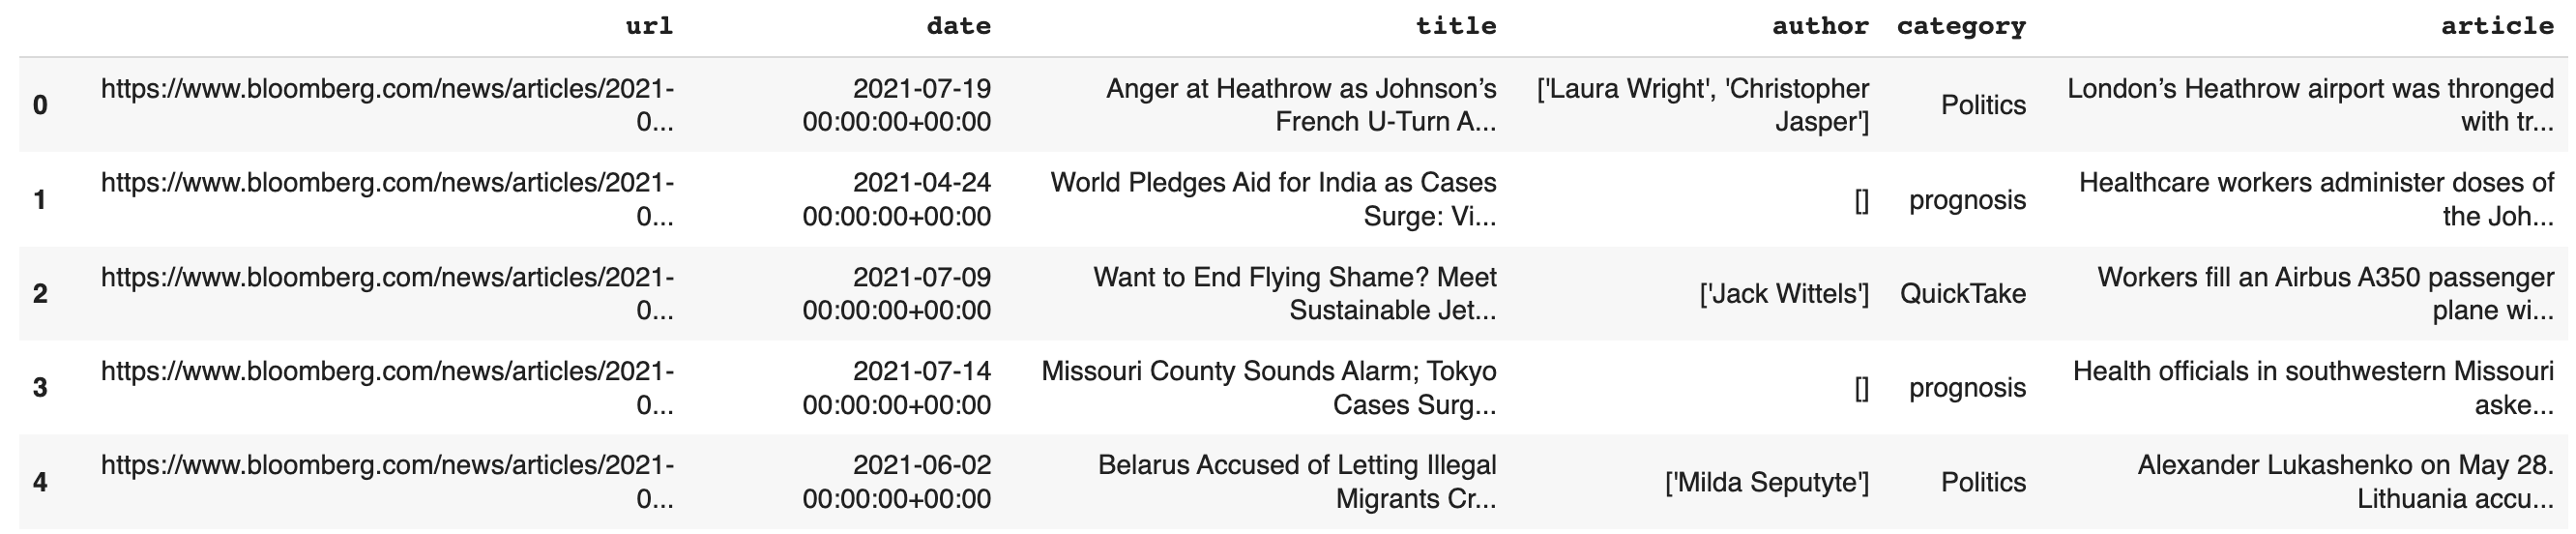
\includegraphics[width=0.8\linewidth]{images/dataframe.png}
\caption{Example data format}
\label{dataframe}
\end{figure}

The objective was to analyse the semantic information in the news articles for each category within a specific time interval. This prompted the need to divide the data meaningfully and was done by grouping the articles by time intervals of a year using `date published' column as well the existing categories that stayed constant to act as a control scaffold. Therefore, an input data group consisted of the articles in a specific category (e.g. Business) during a specific time interval (e.g. 2021). The motivation behind this was to see how news in certain categories changes over time in terms of topics extracted as well as information derived from semantic triples within these topics.

Once these '(Year, Category)' groups were obtained, they were filtered based on their size (i.e., the number of member articles) by omitting all those whose size was less than the $| mean - standard \ deviation |$ of the size of all groups. \hl{The reason for using the absolute difference between the mean and deviations of the value counts of the groups was because variance in the value counts of these groups was too high. Therefore, the aim was to retain the larger year-category groups but omit the really small ones.} This ensured that the input data was of a significant size in order to yield relevant results before any further processing was done.  

% architecture overview
\section{System Design}

\begin{figure}[H]
\centering
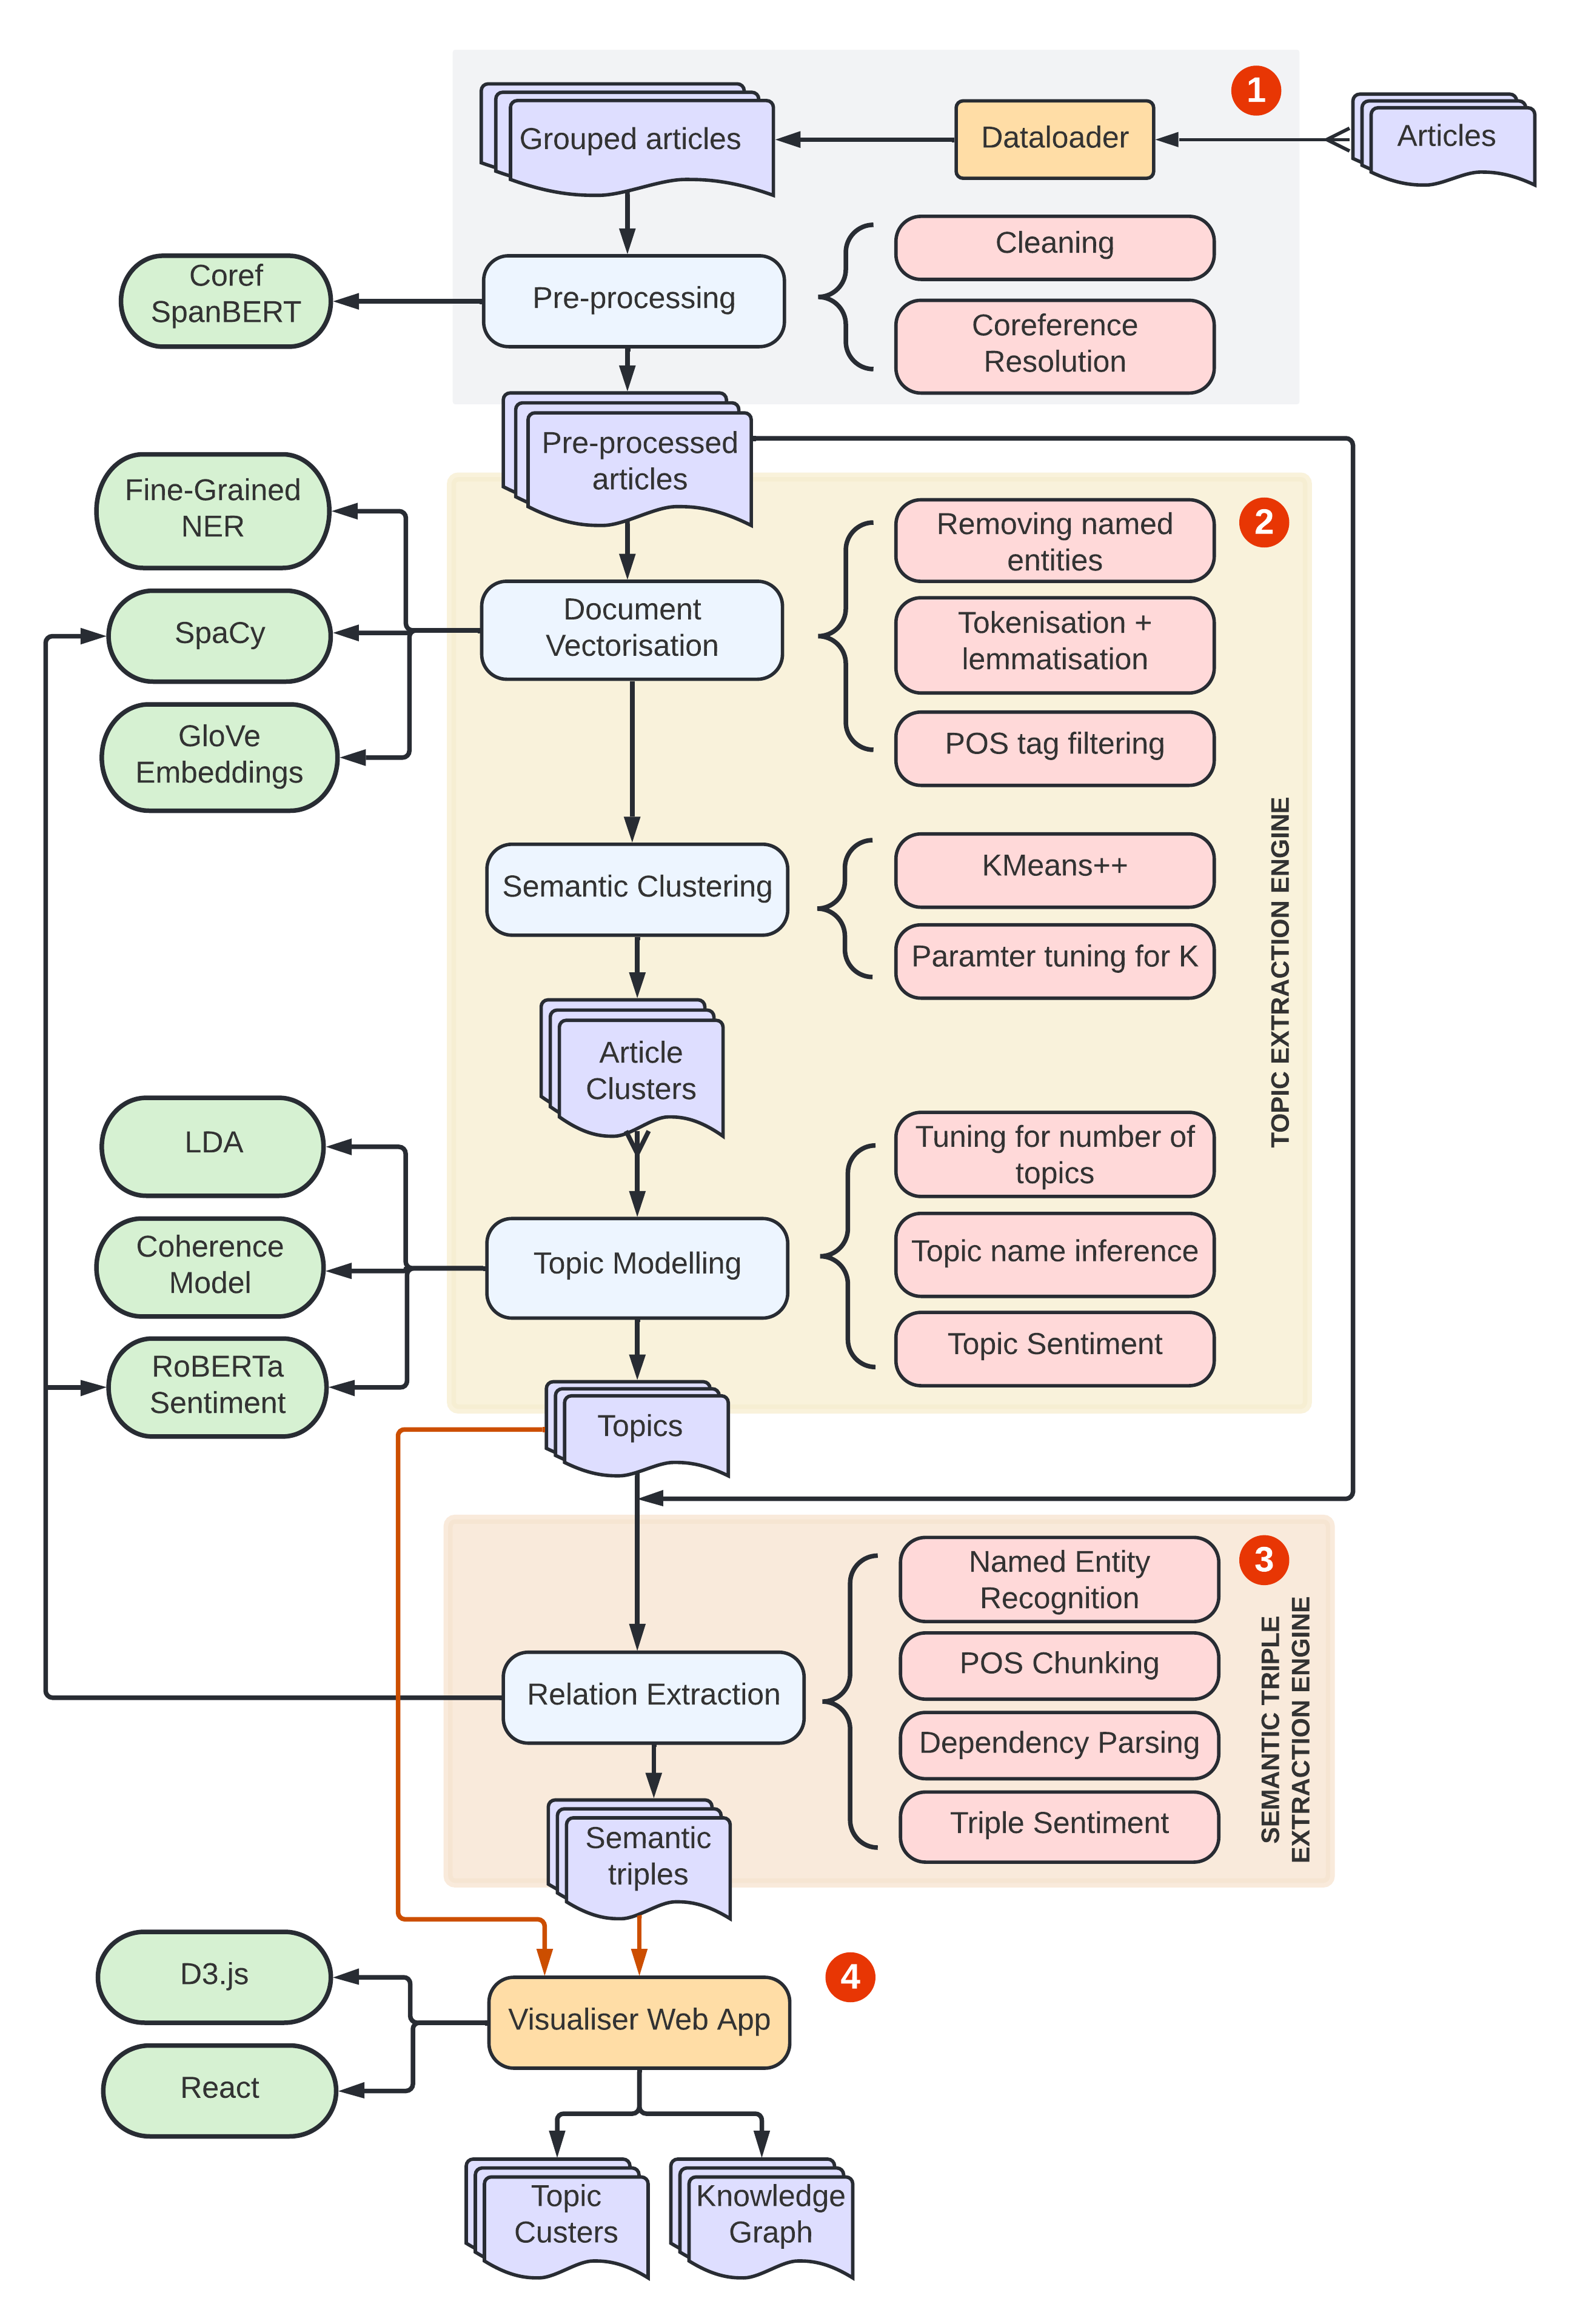
\includegraphics[width=0.7\linewidth]{images/system_arch.png}
\caption{System Architecture Diagram}
\label{fig:sys_arch}
\end{figure}
At a high level, the tool's main goal is to perform semantic analysis on the news corpora to extract information such as topics and semantic triples from the articles. Figure \ref{fig:sys_arch}, shows a high level architecture diagram which follows the pipeline of the semantic analyser tool which follows 4 key stages: 

% of loading data, passing the input groups to the topic extraction engine, using the output latent topics as input for the semantic triple extraction engine, and finally, displaying the outputs from these engines as graphs in a web application. 

\begin{enumerate}
    \item \textbf{Data preparation: }The year-category data groups are generated from the dataset by the \texttt{dataloader} as discussed in \ref{dataloader}. Each input data group then follows the pipeline of pre-processing $\rightarrow$ topic extraction $\rightarrow$ semantic triple extraction engine. 
    
    \item \textbf{Topic Extraction Engine:} This involves semantic clustering of the articles, from which latent topics are extracted. These topics undergo processing such as topic name inference, keyword extraction and sentiment analysis to obtain semantic information about these topics.
    
    \item \textbf{Semantic Triple Extraction Engine:} For each of the semantic  clusters, the semantic triple extraction engine extracts triples of type subject-predicate-object about entities in the article corpus. 
    
    \item \textbf{Visualisation App: } Finally, the semantic clustering and latent topic models are visualised in circle packing graph and the semantic triples are visualised using a force directed graph using D3.js. 
    
\end{enumerate}
\section{Technologies used}
\subsection{Libraries} \label{libraries}

\textbf{SpaCy} is an open-source NLP library "designed specifically for production use" \cite{spacy}. It uses state-of-the-art pre-trained models and in-built pipelines for data processing techniques such as tokenisation, dependency parsing and POS tagging etc. The motivation for using this over other alternatives such as NLTK, was that it was much faster than NLTK for word tokenisation and POS-tagging. Additionally, the NLTK API is quite primitive in comparison to the object-oriented spaCy and requires a lot of unnecessary string manipulation \cite{spacy-nltk}. The spaCy pipeline is trained on several models. For this project, the pre-trained English \hl{en-core-web-lg model} was used with a large word vector table with approximately 500,000 entries.  

\textbf{Gensim} is an NLP open-source library that makes use of state-of-the-art models for word vectorisation, text similarity and topic modelling. For this project, this library was used for the pre-trained models it exposes, in particular, \texttt{Word2Vec} and \texttt{GloVe} and for topic modelling for which the Latent Dirichlet allocation (LDA). 

\textbf{AllenNLP} is an open-source NLP library built on PyTorch and offers variety of well-engineered existing state-of-the-art model implementations \cite{allennlp}. Additionally, it is well integrated with components from the spaCy library such as the \texttt{Tokeniser} and \texttt{SentenceSplitter}, making it a fitting choice for this project. 

\textbf{D3.js} is a JavaScript library which is commonly used for building data visualisations in the web browser. This was used in conjunction with React to build the web application for the visualisation tool. The motivation for using this library over several other alternatives was its data-driven approach to DOM manipulation which enables building customisable interactive visualisation frameworks. 

% \textbf{Ray} is an easy-to-use, fast distributed execution framework. It is designed to scale programs using state of the art ML libraries. This was used over the Python multiprocessing library as this provides a clean way to store memory intensive models in shared memory and run the functions tagged remote asynchronously giving a major performance gain.

\subsection{Models}

Given the extensive prior research in literary analysis and natural language processing, the decision was made to use some of the state-of-art pre-trained models which have proven to be useful in other domains for this problem. The models used in different parts of the project are as follows: 

\textbf{SpanBERT for Coreference Resolution} is a state-of-the-art model used for co-reference resolution developed by the Allen Institute of Technology. It uses the SpanBERT embeddings to get "high-order coarse-to-fine" predictions of spans of text \cite{spanBERT}. The motivation for using this over its predecessor BERT was that SpanBERT outperforms it for the coreference resolution task as it masks random contiguous spans of text unlike BERT which masks random tokens in a sequence, resulting in improved span predictions. The model scores these predictions to get coreference clusters which are applied to get the resolved text \cite{spanBERT}.

\textbf{RoBERTa Stanford Sentiment Treebank} is a binary classifier trained on RoBERTa large for Stanford Sentiment Treebank dataset, on which it achieved 95.11\% accuracy \cite{roberta}. RoBERTa is another variant of BERT and stands for a Robustly Optimised BERT approach. Where BERT is optimised for Masked Language Model task (MLM) and Next Sentence Prediction (NSP), RoBERTa forgoes the latter and only minimises the loss for MLM. Additionally, it uses dynamic masking (i.e., different parts of the sentence are masked for each epoch) instead of static masking (i.e., the same parts of the sentence are masked each epoch) \cite{roberta}. 

\textbf{Fine-Grained NER} is a state of the art named entity recognition model from AllenNLP and is a re-implementation of the Lample (2016) \cite{lample} model. It makes use of bi-direction LTSM with a Conditional Random Field layer (CRF) and uses two types of embeddings: character embeddings and ELMo embeddings (refer to Sections \ref{named_ents} and \ref{elmo}). In Lample (2016), a comparison study for the performance of the model for English NER on CoNLL-2003 test set highlights that it outperforms several other models giving an F1 score of 90.94\% \cite{lample}. The motivation for using this model was this high accuracy and that the model identifies a broad range of 16 semantic types.

\subsection{Web deployment}
A web interface was used for displaying the results of the semantic analysis tool as it allowed for more succinct and cohesive visualisations and enabled user testing. This was accomplished by using React and D3.js to build stateful visualisations. In the latter stages of the project, the website was hosted on Heroku \cite{heroku} which was a scalable approach to accommodate user testing and aided in the evaluation discussed in Section \ref{s:user_eval}.
\chapter{Topic Extraction Engine}

The semantic analysis tool focused on 2 main text mining components in order to extract information from the news articles. This section focuses on the first of these components: the topic extraction engine, covering different data processing techniques, word and document approaches, semantic clustering and topic modelling using LDA. 

\section{Data Processing} \label{s:procesing_topic_engine}

The prepared data (from~\Cref{dataloader}) grouped by (Year, Category) comprised of a list of articles that were published in that year and assigned that category. Processing all the text for every single article would add an intensive computational burden without a huge amount of added benefit, with a potential risk of cluttering the model. For the sake of brevity, the aim was to use the article data most representative of the article. To facilitate this, a decision was made to use the titles and introduction of the articles as they contain the core information in the articles. The introduction of the article (`intro') was extracted as the first \hl{6} sentences of the article using spaCy's \texttt{SentenceSplitter}. Throughout the course of this chapter, `intro' and `article' will be used inter-changeably to represent a single news article in the corpus. 

Once the article introductions are extracted, they then undergo pre-processing before they can be vectorised for clustering. This section highlights the different pre-processing steps and key decisions made to convert the article intros into a list of tokens for the vectorisation step.

\subsection*{Coreference Resolution} \label{coref}
The first step involves coreference resolution of the articles (`intros'). This involves using the pre-trained AllenNLP SpanBERT coreference resolution model for finding the set of mentions in the text that refer to the same `entity' (i.e. coreference clusters). This step was performed on the complete article intro in order for the mentions to be resolved throughout the entirety of the intro and not just on a sentence level. For example, for the text `Sean Doyle is the CEO of British Airways. Prior to this, he was the CEO of Air Lingus', if the coreference resolution was done on the sentence level, the model would miss out on resolving `he' in the second sentence to `Sean Doyle'.

\subsection*{Cleaning Data} \label{data_cleaning}
Post coreference resolution of the article intros, the data needed to be `cleaned' in order to ensure that the news articles retrieved were informative and useful. This involved the following steps: 
\begin{enumerate}
    \item Removing any unnecessary characters e.g., trailing ellipsis, parenthesis etc.
    \item Removing stopwords. The spaCy model's default stopwords list was used. This significantly reduced the amount of text per article intro by removing words such as this, `that', `there', `where', `are' etc. This alone, however, was not sufficient. Given the nature of online news articles, there were some prominent phrases that showed up in several articles, e.g., \qd{Read here}, \qd{For more information}, \qd{Sourced by} etc. These were also removed as they do not provide any relevant information specific to the article, thereby reducing redundancy.

\end{enumerate}

\subsection*{Named Entity Recognition}
As mentioned previously, the aim of these pre-processing steps was to obtain a \texttt{filtered\_tokens} list for each article intro which would be vectorised to represent an article as a vector for clustering. A key decision made was to remove all corresponding named entities form article intro in order to remove any dependency of the topics on these named entities. Eliminating this dependency resulted in better silhouette scores and coherence scores for semantic clustering and topic extraction as detailed in~\Cref{s:preprocess_clustering} and~\Cref{s:preprocess_topic} respectively. 

This step was done before tokenisation as named entities can often be a collection of words such as ``British Airways", ``Paul Sweeney", ``New Haven" etc. and removing these post-tokenisation would not be ideal as they would lose their semantic meaning as tokens. For instance, post tokenisation, the model would try to remove `New', `Haven' from the article intro. Therefore, regex patterns were used to remove all the occurrences of the extracted entities in an article. This included removing all entity types which included but were not limited to, `PER', `LOC', `DATE', `ORG'. This also had a performance gain over the post-tokenisation approach as it avoided the lookup for each token against the unwanted entity tokens list.

The process of extracting these entities from the article corpus using the Fine Grained NER model (refer~\Cref{s:models}) and the BILOU encoding scheme for NER is detailed in~\Cref{alg:named_ents}.

\begin{tabularx}{\textwidth}{X X X X X} 
  \textbf{B} & \textbf{I}  & \textbf{L}  & \textbf{O}  & \textbf{U} \\
  beginning & inside & last & outside &  unit \\
  \end{tabularx}

The output from the NER model gives a set of words and their corresponding entity tags. In essence, the algorithm shows the process of joining the entity tokens to build the entity phrases starting from the `beginning' token until the `last' token. Words with `Outside' as a tag mean that the word is not an entity while `unit' refers to single word entities.  

\begin{algorithm}[H]
  \caption{Extract Named Entities}
  \label{alg:named_ents}
  \begin{algorithmic}   
  \State $entities \leftarrow empty \ set$
  \State $words, tags \leftarrow \text{ner\_model.predict}(sentence)$
  \ForAll{$word, \ tag$ $\in$ zip($words, tags$) } 
    \If{t == `O'}  \State {continue}  \EndIf
    \State $ent\_position, ent\_type$ = tag.split(`--')
    \If{t == `U'} 
    \State{$entities$.add($word$)}
    \Else
      \If{ $ent\_position$ == `B'} 
      \State $ent := word$
      \ElsIf { $ent\_position$ == `I'} 
      \State  $ent := ent + word$
      \ElsIf { $ent\_position$ == `L'} 
      \State  $ent := ent + word$
      \State{$entities$.add($ent$)}
      \EndIf
    \EndIf
  \EndFor
\end{algorithmic}
\end{algorithm}

\subsection*{Filtering Tokenised Data} \label{filtered_tokens}
Once the data was cleaned and void of the pre-determined entity types, the article intros were tokenised and normalised. This was done using the spaCy library's \texttt{Tokeniser} and \texttt{Lemmatiser} pre-trained on the English language model: \hl{en\_core\_web\_lg} (refer to~\Cref{libraries}). Normalisation was done through lemmatisation (to obtain the base forms of the tokens). This was chosen instead of stemming as it guaranteed more semantically meaningful tokens which for reasons detailed in~\Cref{normalisation}. The process of obtaining a list of tokens for each article intro was as follows:
\begin{enumerate}
    \item Each sentence in the intro was turned into a list of tokens.
    \item These tokens were filtered by their Part-Of-Speech (POS) tags against the allowed POS tags, which was restricted to nouns (`NOUN').
    \item Tokens that were numeric and less than 2 characters were also removed. 
    \item The remaining tokens were lemmatised and added to the \texttt{filtered\_tokens} list for the given article.
\end{enumerate}

It is important to note that the allowed POS tags were originally set to include nouns (NOUN), adjectives (ADJ), verbs (VERB) and adverbs (ADV). This resulted in a lot of unnecessary tokens such as ‘because’, ‘did’, ‘very’ etc. Different combinations of the allowed POS tags were experimented with, ultimately allowing only nouns to comprise the \texttt{filtered\_tokens} for each article (`intro'). This decision was primarily based on the resulting clustering scores when the allowed POS tags were limited to `NOUN' and when they included `NOUN', `ADJ', `VERB' and `ADV' as discussed in the evaluation in~\Cref{s:pos_clustering}.

\section{Semantic Clustering} \label{s:semantic_clustering}

The first step to generating semantic clusters of articles is to get the corresponding article vectors. This involves vectorising the individual tokens in \texttt{filtered\_tokens} list for each article intro.

\subsection{Word embedding approaches} \label{word_embed_approaches}
To vectorise the tokens, different pre-trained word embedding models were used. These approaches (in chronological order) with their strengths and shortcomings are outlined below.

\renewcommand\arraystretch{2}
\captionsetup{singlelinecheck=false, labelfont=sc, labelsep=quad}
\begin{longtable}{@{\,}r <{\hskip 2pt} !{\foo} >{\arraybackslash}p{13cm}}
\centering

TF-IDF & Term frequency-inverse document frequency is a statistical metric that examines the comparative relevance of a word/token with respect to an article intro in the collection of articles. Representing the tokens as their TF-IDF measure first involves calculating the term frequency (TF) using the bag of words (BoW) approach from Gensim \texttt{Doc2BoW}. To account for overlapping terms across all article intros, the term frequency was multiplied by the inverse document frequency to weigh down the terms whose high frequency is not unique to a document (Refer to  \hl{Add in BCKG}). A dense document-term using the TF-IDF values for each term is used to represent the article intro as a vector for clustering. \\

Word2Vec & The next approach saw the use of Google's \texttt{Word2Vec} model (from Gensim) to obtain pre-trained word embeddings for each token in an article's corresponding \texttt{filtered\_tokens} list. The issue with the previous approach was that it represented the statistical information about a document, in particular, the measure of the frequency of words in a document, rather than any semantic information about a document. \texttt{Word2Vec} embeddings, on the other hand, return a vector for each word that accounts for semantic similarity (based on cosine distance) between the words represented by the vectors~\cite{word2vec}. \\

GloVe & The final approach was to use Stanford's \texttt{GloVe} (global vector) embeddings from Gensim. \texttt{GloVe} as been pre-trained on Wikipedia and Gigaword 5, consisting of a vocabulary of 400,000 words which are represented by 300 dimensional vectors~\cite{glove}. The advantage of this approach over previous approaches is that it makes use of global statistics such as word co-occurrences to obtain word vectors. Using these embeddings also saw an improvement in the silhouette scores when deriving the semantic clustering of articles as detailed in~\Cref{s:word_embeddings}. \\
\end{longtable}

\subsection{Document embeddings}

In~\Cref{filtered_tokens}, \texttt{filtered\_tokens} are defined as the all \textit{relevant} tokens for each article intro. As mentioned above, the filtered tokens were vectorised using the \texttt{GloVe} embeddings~\cite{glove} resulting in a list of vectors corresponding to the \texttt{filtered\_tokens}. In order to get the document vectors from these word vectors, two approaches were tested: 

\renewcommand\arraystretch{2}
\captionsetup{singlelinecheck=false, labelfont=sc, labelsep=quad}
\begin{longtable}{@{\,}r <{\hskip 2pt} !{\foo} >{\arraybackslash}p{13cm}}
\centering

Approach 1 & The corresponding tokens in \texttt{filtered\_tokens} list for the article intro are vectorised (using \texttt{GloVe} embeddings) and averaged to find the corresponding article vector. This was a simple approach that gave equal importance to each token associated with the article intro. \\

Approach 2 & Rather than simply averaging the token vectors for each article intro, the document vector was calculated using a weighted sum of corresponding word vectors (from \texttt{filtered\_tokens}). This was done by using a TF-TDF model to get the term-frequency inverse document frequency weight for each token in the corresponding article. This meant that words that appeared in high frequency unique to the associated article contributed more to the document vector than those with a lower frequency or those that appeared frequently in other article intros. \\

Approach 3 & Building on the previous approach, this method selects the top 10 most representative words based on the TF-IDF weightings and performs the weighted average to generate the article vector.\\
\end{longtable}

\begin{figure}[H]
  \centering
  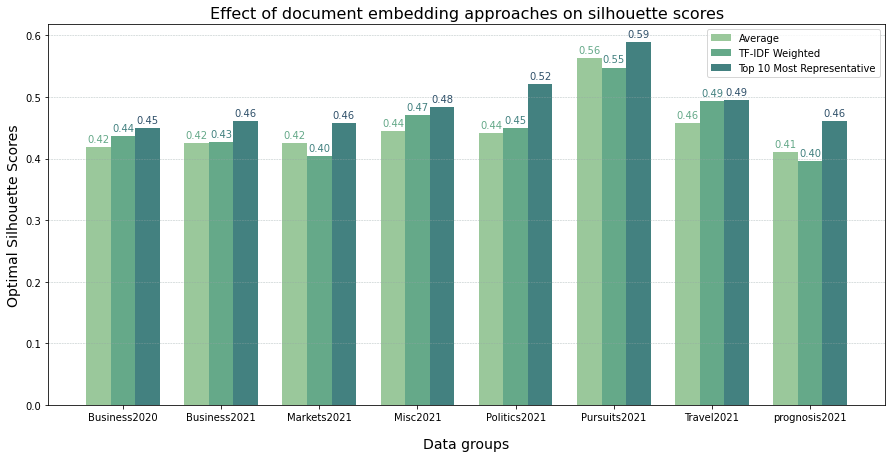
\includegraphics[width=0.8\linewidth]{images/eval/doc_embedding_sil.png}
  \caption{Effect of the different document vector generation approaches on the semantic clustering silhouette scores}
  \label{fig:doc_embeddings}
  \end{figure}

  \vspace{-2em}
\Cref{fig:doc_embeddings} shows how the different word embeddings approaches effect the `goodness' of clustering indicated by silhouette scores. The consensus derived is that Approach 3, which describes calculating the article (document) vector by computing the weighted average of the top 10 most relevant words (using the TF-IDF metric), performs better than the other 2 approaches mentioned. Approach 3 results in a 9.36\% improvement in silhouette score compared to Approach 1 (simple averaging of word vectors) and an 8.37\% improvement compared to Approach 2 (weighted (TF-IDF) average of all word vectors). This led to the decision of using Approach 3 as the method for document vector generation. \hl{Figure out how to add the silhouette score stuff before?}

%%%%%%%%%%%%%%%%%%%%%%%%%%%%%%%%%%%%%%%%%%%%%%%%%%%%%%%%%%%%


\subsection{Dimensionality Reduction}

\subsubsection{Normalising Data}
The first step is to normalise the article vectors in order to eliminate redundancy in data and standardise the features (components of the vector) in case of high variance, which contributes to better clustering. Additionally, when it comes to performing principal component analysis for the article vector, we want the features (in vectors) to be independent of their standard deviation or variance. This is necessary to get a good covariance matrix among the features.  

\subsubsection{Principal Component Analysis}

As established previously (refer to~\Cref{word_embed_approaches}), \texttt{GloVe} document embeddings result in a 300-dimensional vector. Clustering the document vectors becomes inefficient and meaningless at these high dimensions as the concept of distance becomes less precise as the number of dimensions increases~\cite{pca_clustering} as the volume of space increases exponentially making the available data spare - curse of dimensionality. For any given point in this high n-dimensional space, the difference in 'distance' (euclidean) to the closest point $d_min$ and the farthest point $d_max$ with respect to the $d_min$ becomes negligible~\cite{nearest_neighbour}. 

\[ \lim_{n\to\infty} \frac{d_{max} - d_{min}}{d_{min}} \to0\]

The concept of clustering these articles relies on grouping similar articles together based on their attributes. The similarity is determined based on the vectorised \texttt{filtered\_tokens}. However, given the high dimensional nature, some of these attributes will not be relevant in determining these clusters. The goal is to find the attributes (vector components) with the most variance across the documents vectors to represent the features. This is accomplished by performing principal component analysis (PCA) on the normalised high-dimensional input vector space to map to a low dimensional space, whilst minimising information loss~\cite{pca_clustering}.

\begin{figure}[H]
  \centering
    \begin{minipage}[t]{.49\textwidth}
      \centering
      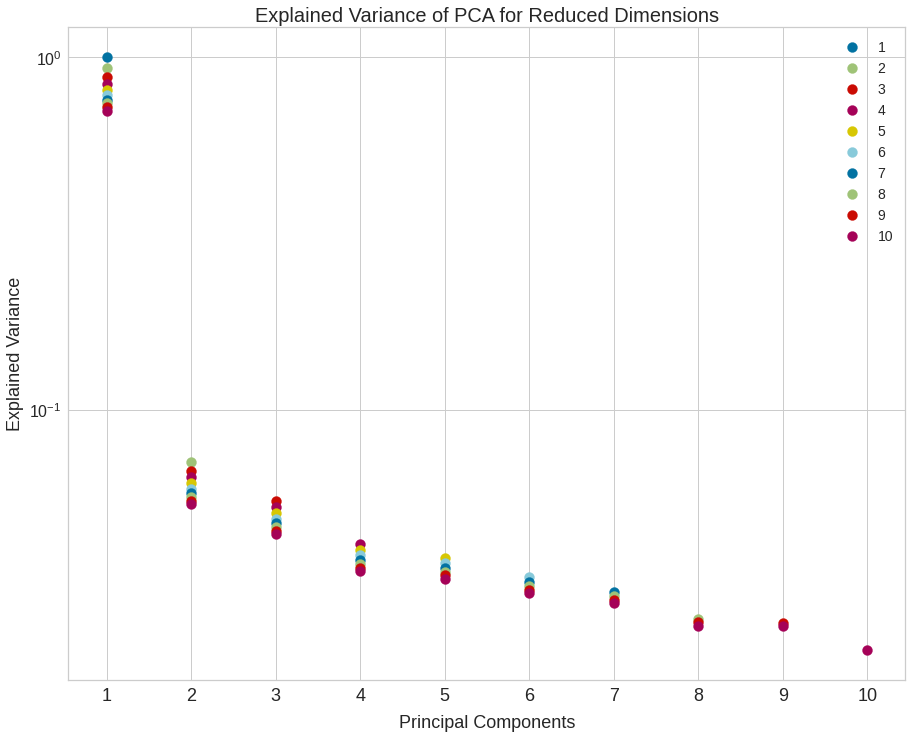
\includegraphics[width=\textwidth]{images/eval/explained_variances.png}
      \caption{-}
      \label{fig:explained_variance}
    \end{minipage}
    \begin{minipage}[t]{.49\textwidth}
      \centering
      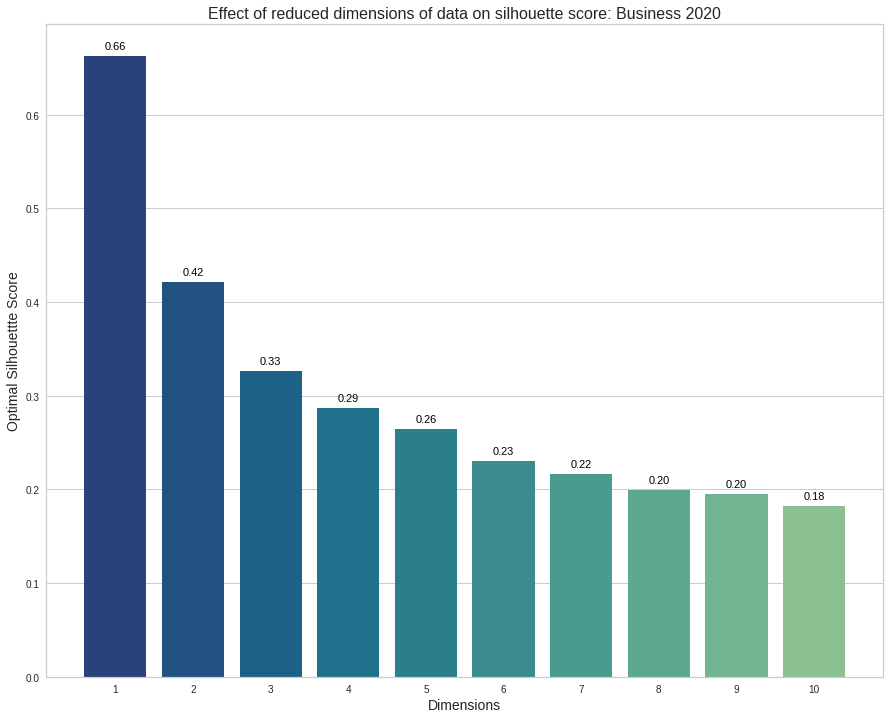
\includegraphics[width=\textwidth]{images/eval/pca_silhouette.png}
      \caption{-}
      \label{fig:pca_sil}
    \end{minipage}
  \end{figure}

  As seen in~\Cref{fig:explained_variance}, when the article vector space is projected to dimension=1, the variance is explained entirely by dimension 1 (blue dot). As the number of dimensions increase, the number of principal components increase, the main proportion of the variance can still be explained by the first principal components (close to 1). For instance, projecting to dimension=10, the explained variances for each of the 10 principal components is as follows: 
  \begin{table}[H]
      \centering
  \renewcommand{\arraystretch}{1.1}
  \begin{tabularx}{\textwidth}{|X|X X X X X X X X X X|} 
    \hline
    PC & \textbf{1} & \textbf{2}  & \textbf{3}  & \textbf{4}  & \textbf{5} & \textbf{6} & \textbf{7}  & \textbf{8}  & \textbf{9}  & \textbf{10}\\
    \hline
    EV & 0.88 & 0.026 & 0.021 & 0.014 & 0.011 & 0.010 & 0.0094 & 0.0090 & 0.0082 & 0.0074\\ 
    \hline
    \end{tabularx}
  \end{table}
  
  Therefore, 88\% of the variance (EV) can be explained by the first principal component (PC) alone and so the article vector space can be transformed using PCA with dimensions=1.~\Cref{fig:pca_sil} shows the effect of transforming the article vector space to different dimensions on the silhouette scores, which represent the `goodness of clustering'. It indicates that transforming the vectors to a single dimension (using PCA) result in the highest silhouette score. Therefore,~\Crefrange{fig:explained_variance}{fig:pca_sil} conclude that the setting the dimension to 1 for PCA transformation results in the most optimal clustering whilst retaining majority of the information (variance).

\subsection{KMeans Clustering}
Once the normalised data is mapped to the lower subspace, the documents (article intros) are clustered based on similarity. The aim is to cluster the article intro vectors based on their cosine similarity~\cref{eq:cosine_sim} using cosine distance as the distance function~\cref{eq:cosine_distance}. The clustering technique used was KMeans clustering. This was done using the \texttt{sklearn} library's \texttt{kmeans} function with `euclidean distance'~\cref{eq:euc_distance}. This was feasible given the linear relationship between Euclidean distance and  cosine distance~\cite{kmeans} for normalised vectors as in shown in~\cref{eq:relationship_ce}.


\begin{align}
  \mathit{For \ normalised \ vectors,} \ x, y:  \sum x_i^2 &= 1,  \sum y_i^2 = 1 \label[equationX]{eq:normalised} &\\ 
  \mathit{Cosine \ Similarity,} \ cos(x, y) &= \frac{\sum x_i y_i}{\sqrt{\sum x_i^2 y_i^2}}  \nonumber &\\ 
   &= \sum x_i y_i \label[equationX]{eq:cosine_sim} &\\
   \mathit{Cosine \ Distance} &= 1 - cos(x, y) \label[equationX]{eq:cosine_distance} &\\
   \mathit{Euclidean \ Distance,} \ || x - y ||_2^2  &= \sum (x_i -  y_i)^2  \label[equationX]{eq:euc_distance} &\\
                 &= \sum (x_i^2 + y_i^2 - 2 x_i y_i)  \nonumber &\\
                 &= \sum x_i^2 + \sum y_i^2 - 2\sum x_i y_i   \nonumber &\\
                 &= 1 + 1 - 2 cos(x, y)  \nonumber &\\
                 &= 2 (1 - cos(x, y))  &\\
                 &= 2 (\mathit{Cosine \ Distance}) \label[equationX]{eq:relationship_ce}
\end{align}


% \todonum[inline, color=darkgray]{Add kmeans formula - MDS?}

Furthermore, to avoid falling into the trap of random centroids initialization, a major shortcoming of the KMeans method, the clustering was done with KMeans++. KMeans++ offers a better initialisation approach for centroids, in which the first one is picked at random and the subsequent centroids are chosen with a probability proportional to the squared distance from the closest chosen centroid.


\subsection*{Determining the optimal number of clusters}
Determining the number of clusters (k) in KMeans is a crucial factor to consider. This was done by computing the KMeans clustering algorithm for different values of k varying from 2 (minimum number of clusters) to m (maximum number of clusters), and picking the optimal k based on a comparing statistic. The two comparison statistics considered were: Elbow method with Within Cluster Sum of Square distance (WCSS) and Silhouette score. 

\subsubsection{Method 1: Minimising WCSS using Elbow Method}
The elbow method uses the distance (Euclidean) between the cluster centroid and its members, i.e., intra-cluster variance (distortion score or WCSS) to determine how many clusters are needed to encapsulate the variance of the data. In particular, it minimises the loss function: WCSS (a.k.a. distortion score) which is the sum of the squared distance between each point and the centroid in a cluster~\cite{elbowvssil}.
\vspace{-1ex}
\begin{align}
  \mathit{WCSS} &=  \sum^{C_n}_{C_k} (\sum^{d_m}_{d_i \in C_i} || d_i - C_k ||_2^2) \label{eq:wcss}
\end{align}

As seen in~\Cref{fig:elbow}, the elbow (bend) in the plot determines the optimal number of clusters, i.e., the k value = 4. The main drawback of using the lowest distortion score to determine the optimal number of clusters is that as long as the number of clusters (k) increases, the distortion score (WCSS) will decrease because the points will be closer to their centroids. Hence, the elbow (bend) is used to determine the minimum number of clusters with a reasonably low distortion score as seen in~\Cref{fig:elbow}, which gives the optimal number of clusters, k=4.

\begin{figure}[H]
\centering
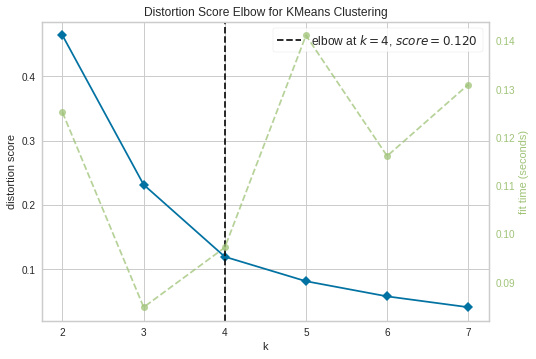
\includegraphics[scale=0.4]{images/elbow.png}
\caption{`Business 2020' Elbow Method Plot for k=2..7}
\label{fig:elbow}
\end{figure}

\subsubsection{Method 2: Silhouette score}

The second approach involved using the silhouette score. Unlike, the elbow method silhouette score accounts for both how close a point is within its cluster (cohesion)~\cite{elbowvssil} and other clusters (separation)~\cite{silhouette}.

\begin{center}
    $\mathit{Silhouette \ Score }= \mathit{mean}_i (\frac{S_i - C_i}{\max(S_i, C_i)}) $
\end{center}
% \ mathrm
where 
cohesion, $C_i$ = average distance between i and all points within its cluster.
separation, $S_i$ = average distance between i and all points not in its cluster.

The silhouette score is the mean of Sil(i) for all points i in the data. It ranges from -1 to 1. A value closer to 1 indicates that clusters are well separated and distinguished. A value ~ 0 indicates significant overlapping between the clusters, and the clusters are not distinguished. A value near -1 indicates that clusters are assigned incorrectly.

\begin{figure}[H]
\centering
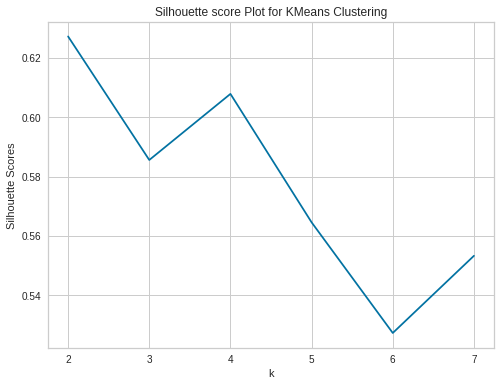
\includegraphics[width=0.4\linewidth]{images/sil_kmeans_.png}
\caption{`Business 2020' Silhouette Plot for KMeans clustering with k=2..7}
\label{fig:sil_kmeans}
\end{figure}
\vspace{-2ex}

\begin{figure}[H]
\begin{minipage}{0.45\linewidth}
\centering
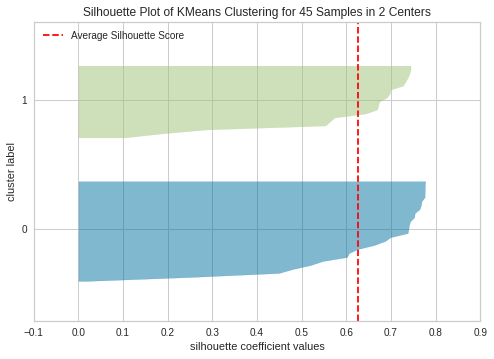
\includegraphics[width=\linewidth]{images/cluster 2.png}
\caption{`Business 2020' Silhouette Diagram: score = 0.627 for k=2}
\label{fig:cluster2}
\end{minipage}
\hfill
\begin{minipage}{0.45\linewidth}
\centering
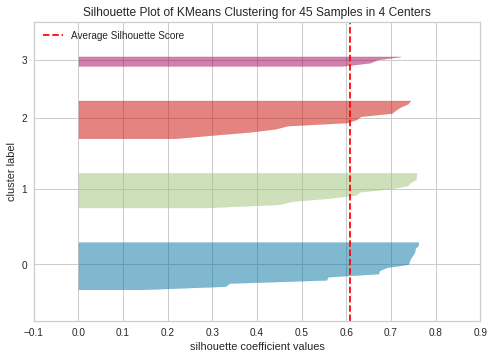
\includegraphics[width=\linewidth]{images/cluster 4.png}
\caption{`Business 2020' Silhouette Diagram: score = 0.607 for k=4}
\label{fig:cluster4}
\end{minipage}
\end{figure}

\vspace{-1ex}
From~\Cref{fig:sil_kmeans}, it is apparent that while selecting k=4 (as found by Elbow Method in~\Cref{fig:elbow}) results in a good clustering, a better clustering can be achieved by selecting k=2, as it gives a higher silhouette score, suggesting less overlap. \Crefrange{fig:cluster2}{fig:cluster4} show the silhouette diagram for number of clusters, k=2 and k=4 respectively. The cluster thickness denotes the size of the cluster, while the width represents the sorted silhouette coefficients of instances in the cluster. Observing~\Cref{fig:cluster2} (k=2) reveals that both clusters are roughly equal in size, whereas~\Cref{fig:cluster4} (k=4), illustrates a higher disparity in size as Cluster 3 is less than half the size of others. This is indicative of some clusters being split, thereby resulting in a suboptimal silhouette score. 

Out of the two approaches, the decision was made to go with the silhouette score as it factors both how compact a cluster is and how distinct it is. This is a vital consideration given that the aim of the engine is to distinctly cluster the news articles with minimal overlap, in order to minimise common topics within clusters post topic modelling (performed on each cluster). 

\subsection*{Find n most representative docs} \label{sec:Find_n_docs}

Once the articles are clustered, the goal is to obtain a cluster-to-article mapping. However, given the high volume of data, it is not as necessary to consider every single article in the cluster particularly those that are not close to their respective cluster centroids. A pre-determined value $n_{max}$ is selected, and the euclidean distance from each member (article) to its centroid is computed. The articles are sorted in increasing order of distance and the top n articles are selected for each cluster. Furthermore, since the next step in the topic extraction engine entails modelling topics on these semantic clusters, it is futile to consider the sparse clusters that have very few (less than $n_{min}$) members as they will not spawn any good topics and are therefore omitted. These values $n_{max}$ and $n_{max}$ are calculated based on the mean and standard deviation of the sizes of semantic clusters obtained as shown in~\crefrange{eq:nmin}{eq:nmax}.
\vspace{-1px}
\begin{align}
  n_{min} &= \lfloor mean(|C_1|, |C_2|, ..., |C_n|) - std(|C_1|, |C_2|, ..., |C_n|) \rfloor \label[equationX]{eq:nmin} &\\
  n_{max} &= \lceil mean(|C_1|, |C_2|, ..., |C_n|) + std(|C_1|, |C_2|, ..., |C_n|) \rceil \label[equationX]{eq:nmax}
\end{align}

\section{Topic Modelling}

Post semantic clustering, the aim is to extract topics associated with each cluster. This was done through topic modelling, which follows an unsupervised approach of extracting the top topics from a corpus. In particular, the model used was the Latent Dirichlet allocation (LDA) from the Gensim library. 

As explained in~\Cref{Topic Modelling appoaches}, each document (article intro) is made up of several words (\texttt{filtered\_tokens}) and each topic has several (key)words associated with it. Given that the LDA model is a probabilistic model, it tries to estimate the topic distribution for each article as well as the word distribution for each topic. The motivation for using LDA is to get the topic-document probability distribution which can then be used to get the topics associated with a document. For the scope of this problem, this was limited to one dominant topic. 

It is important to note that topic modelling LDA does not rely on semantic information, this is why the decision was made to obtain semantic clusters first and then model topics on them.
\vspace{-1ex}
\subsection{Corpus Decisions}

From the data processing steps detailed in~\Cref{procesing_topic}, the article intros have already been cleaned, lemmatised, filtered and tokenised to get their corresponding \texttt{filtered\_tokens}, which are void of any stopwords and named entities and only contain nouns. For the input corpus passed to the LDA, there were certain key decisions made, which were influenced by previous studies and quantitive evaluation (discussed in \Cref{s:evaluation_topic_extraction}). Using the \texttt{filtered\_tokens} satisfied most of these requirements which are explained below: 

\begin{enumerate}
  \item \textbf{Noun-only corpus}: Based on previous studies~\cite{nouns_only_lda}~\cite{efficient_noun_only_approach}, and the results from~\Cref{s:pos_topic} which saw improved coherence values of topics averaged across clusters and \hl{fewer numbers of `unpopular' topics (i.e. those with few associated articles)}, the decision was made to limit input corpus to nouns (satisfied by \texttt{filtered\_tokens}). This aligned with the intuition that nouns are better indicators of a topic as they provide more semantic context. Opening the corpus to other POS categories, for instance, ADJ, VERB (Appendix~\Cref{appendix:pos}), will result in sub-optimal topics since the LDA model will give "fast" and "pandemic" equal importance.
  
  \item \textbf{No Named Entities}: Similar to semantic clustering, the decision as made to omit all named entities from the LDA corpus. This was also satisfied by the \texttt{filtered\_tokens} where the entities found using the Fine-Grained NER model were removed. As seen in ~\Cref{fig:pos_topic}, omitting named entities improved the coherence score of the topics. 

  \item \textbf{Using Bigrams}: Inspired by \cite[`Beyond bag of words']{bigrams_lda}, a decision made was to augment the corpus using n-grams, in particular, bigrams, rather than solely using unigrams. This allowed the model to consider a combination of two commonly occurring words across documents, e.g., “coronavirus\_pandemic”, “aviation\_industry” etc. This was particularly relevant given the dataset of news articles containing common `noun chunks' which can be used to infer topics. The bigrams are derived using Gensim's \texttt{Phraser} which uses colocation detection, and are appended to \texttt{‘filtered\_tokens’.}
  
  \item \textbf{TF-IDF}: In LDA, the document need to be transformed into numeric feature vectors which form the corpus. Since it does not rely on the article's semantic information and builds topic estimators based on words, article and topics, it uses frequency vectors as obtained by Bag-of-Words and Term Frequency-Inverse Document Frequency. The decision was made to use TF-IDF over the more common Bag-of-Words~\cite{topic_models}, in an attempt to minimise overlap of topics as each article will be associated with one dominant topic.
\end{enumerate}

% \subsection{Implementation}
% \todonum[inline]{Pseudocode/ Diagram?}
% \begin{enumerate}
%     \item \textbf{Bigrams:} Using Gensim’s Phraser model which uses colocation detection, the bigrams are generated (a\_b where a and b are nouns), which are appended to the ‘filtered\_tokens’.
%     \item \textbf{Corpus:} Based on the decisions highlighted in section ???, the corpus is defined as a collection of filtered, tokenised, lemmatised nouns and noun-chunks (bigrams) of article intros, barring entities and stopwords.
    
%     % <Potentially talk about PMI scoring - PMI-like scoring as described in Mikolov, et. al: “Distributed Representations of Words and Phrases and their Compositionality”.>
    
%     \item \textbf{Dictionary:} A dictionary mapping the words in the corpus to their integer ids is created using the Dictionary \hl{wrapper?} in Gensim. 
%     \item \textbf{BoW, TF-IDF:} The corpus is passed to the bag of words model from Gensim and then is transformed by the TF-IDF to return a weighted frequency of words in article intros. This is the input to the LDA model. 
% \end{enumerate}

% Pseudocode: 
% For each cluster, 
% 	Get articles indexes in the clusters. 
% 	Get the corresponding filtered tokens (ones that were used to vectorise the article in clustering) => dictionary 
% 	Make n grams 

\subsection{Determining number of latent topics}

A key contributor in determining the quality of the topics extracted is tuning the {num\_topics} parameter \texttt which represents number of topics outputted by the LDA. A low value will result in too few or overly generalised topics whereas a high value results in uninterpretable topics that ideally should have been merged~\cite{topic_score}. Previous studies~\cite{cv_abstract}~\cite{cv_space} show that one of the best methods to determine the number of latent topics is to measure CV coherence, which has a high correlation with human judgments of topic interpretability. This metric computes the normalised pointwise mutual information (NPMI) and cosine similarity of content vectors of words, derived based on their co-occurrences~\cite{cv_space}.

This was achieved by using \texttt{CoherenceModel} with the `c\_v' setting from the Gensim library. The optimal number of topics (i.e., value resulting in the highest coherence score) is computed for each cluster by running the LDA model with different values of k varying from min\_topics (defaulted to 2) to max\_topics (dependent on the size of cluster), and the LDA model with the highest resulting coherence is chosen. The motivation for bounding the max\_topics was to ensure topics would have at least the minimum number of article intros (=2). Additionally, pruning the number of LDA runs had performance gain.

\subsubsection*{Dominant Topic-Article Mapping} \label{sec:topic_article_mapping}
Once the optimal value of n\_topics is determined, the corresponding LDA model is applied to the TF-IDF corpus to get the resulting article-topic distribution. This returns the most probabilistic topics for each article intro. This is of the form \texttt{articleId: (topicId, probability)}, where \texttt{probability} refers to the likelihood that the article belongs to the topic corresponding to the \texttt{topicId}. Of these, the most dominant topic (the highest likelihood of belonging to the topic) is selected, resulting in an 1-1 topic-article mapping. 

\vspace{-1ex}
\subsection*{Topic Name Inference}

An augmented feature of the Topic Modelling Engine was to infer the topic names from the keywords of the topic. \Cref{alg:topic_name} details the process of inferring topic names from the corresponding topic keywords. This involves splitting any bigram keywords to obtain a set of keyword tokens which are checked to ensure they are nouns, not a stopword and have an associated \texttt{Glove} vector. Using the \texttt{glove\_model.most\_similar()} method from Gensim, which computes the cosine similarity between an average of projection of resulting keyword vectors (\texttt{validKws}), the candidate topic names are obtained. These are again checked for validity in terms of whether they are a noun and are not augmented stopwords. The top 2 most similar topic name tokens that meet the validity checks are selected as the topic name for the given topic. 

\begin{algorithm}[H]
  \caption{Infer Topic Name}
  \label{alg:topic_name}
  \begin{algorithmic}   
    \Function{GetValidKeywords}{$topicKeywords$, $stopwords$, $allowed\_pos=[`NOUN']$}
    \State $validKws \gets \emptyset$
    \ForAll{$topicKw \in topicKeywords$} 
    \State $kw \gets topicKw.lemma$
    \If {$kw \in stopwords$ \AND $kw \notin GloVe.vocab$ \AND $kw.pos \notin allowed\_pos$}
    \State $continue$
    \EndIf
    \State $validKws.append(kw)$
    \EndFor
    \State \Return $validKws$
  \EndFunction

\vspace{1em}
  \Function{GetTopicName}{$topicKeywords$, $stopwords$}
    \State $kws \gets$ \Call{GetKeywordTokens}{$topicKeywords$}
    \Comment{$splits \ bigrams$}
    \State $validKws \gets$ \Call{GetValidKeywords}{$kws, stopwords$}[:5]
    \State $topicNameCands := \text{GloVe}.most\_similar(validKws, topn=5)$
    \State $validTopicNames \gets$ \Call{GetValidKeywords}{$topicNameCands, stopwords$}
    \If {$len(validTopicNames) == 0$}
    \State \Return $validKws[0]$
    \Else
    \State \Return $validTopicNames[0:2]$
    \EndIf
  \EndFunction
\end{algorithmic}
\end{algorithm}
\vspace{-1ex}
\subsection*{Topic Sentiment}

\begin{algorithm}[H]
  \caption{Computing Topic Sentiment}
  \label{alg:topic_sent}
  \begin{algorithmic}   
  \Function{GetTopicSentiment}{$topicArticles$}
    \State $sentiments \gets  \emptyset$
    \ForAll {$article \in topicArticles$}
    \State $sentiments.append(roBERTA\_model.predict(article.title))$ \Comment{0: N, 1:P}
    \EndFor
    \State $avgSent = average(sentiments)$
    \If {$avgSent >= 0.4 \AND avgSent <= 0.6$}
    \State \Return `Neutral'
    \ElsIf {$avgSent > 0.6$}  \Return `Positive'
    \Else  \Return `Negative'\EndIf
  \EndFunction
\end{algorithmic}
\end{algorithm}
\vspace{-1ex}
The last component of the Topic Modelling Engine involves sentiment analysis. In order to compute the topic sentiment, the snetiment of each article associated with the topic is computed. For this, the RoBERTa Sentiment Treebank model is used on the article title as it serves as good descriptor of the tone of article. The model outputs a binary label, where 0 indicates `negative' sentiment and 1 indicates `positive' sentiment. These are then averaged to get the sentiment of the topic. Based on the range of this value it is assigned one of the following: 'Positive', 'Negative' and 'Neutral' as shown in~\Cref{alg:topic_sent}.

\section{Results and Discussion}
\chapter{Relation Extraction Engine}

This section focuses on the relation extraction engine, covering the journey to the current implementation, focusing on data preparation and the different approaches for extracting semantic triples.

\section{Data Pre-Processing}

Before the relations are extracted from the articles, the articles need to be processed. This involves the coreference resolution and data cleaning to remove stopwords, unnecessary punctuation etc. as discussed in previous sections \ref{coref} and \ref{data_cleaning} respectively. Pre-processing the articles with coreference resolution has the benefit that all the \hl{............}

\todonum[inline]{add stuff}

\section{Motivation}
The motivation behind this \hl{part of the project} was to find a way to extract meaningful information from the article, in particular, information centred around key entities in the article corpus for a certain topic. This subsection covers the two different ideas explored for extracting information from articles. 

\subsection{Cooccurence Graph}
One of the earlier approaches was to derive a co-occurrence graph from the article corpus (pre-processed with coreference resolution and data cleaning) for a selected topic. This was useful in showing what entities were present and how they connected to one another as shown in \hl{Figure} \ref{coocc}. In order to derive the cooccurence graph, Named Entity Recognition (NER) was used. For each article, the \hl{intro} sentences were extracted and on each sentence NER was performed to extract all relevant entities. The types of entities extracted included but were not limited to, 'GPE', 'PER', 'LOC', 'ORG' etc. and excluded 'DATE', 'MONEY', 'TIME', 'CARDINAL', 'PERCENT' and 'QUANTITY' \hl{(See Appendix for reference)}. As seen in Figure \ref{coocc} in Appendix, the the size of the nodes representing the entities were reflective of the number of co-occurrence links (edges) incident to and from other entities. This was done so that for any given topic the most relevant entities, i.e., mentioned the most in the group of articles representing a topic, was apparent. The \textbf{limitation} of this approach, was that while this was a good indicator of general entities talked about in a topic, the amount of information extracted from the topic article corpus was not sufficient and did not provide any explicit information about \textit{'how'} the entities were related to one another, but rather, just simply, that they were.

\subsection{Semantic Triples}
In an attempt to extract more 'relevant' information indicative to the content discussed in articles of a given topic, the decision was made to extract semantic triples from article corpus instead of building a cooccurrence graph. 
This involved finding subject-relation-object triples form the sentences in the article corpora. \hl{??????? better semantic information extraction}
\todonum[inline]{Talk about why the pure dependency parsing method did not go well}
The process of extracting these relations involved inferring both syntactic and semantic dependencies between tokens in a sentence, making use tokenisation, dependency parsing,  part-of-speech tagging and named entity recognition.

\section{Key decisions} \label{key_decisions_rel}
\hl{In order to capture better nodes and relations, phrases are used instead of words. Given an example of teh sentence in figure, are calling for gives better understanding than calling. Also talk about how the knowledge graph is the goal and in particular we want to see the subject as entities to find out all the information about them in articles in a topic.}

\subsection{Relation as verb phrases}

\subsection{Subject as entities} \label{subject_ents}
Given that the end goal is to build a knowledge graph, the nodes must have \hl{common entities so that the graph can display all the different triples about an entity and which entities exist in the article corpus of a given topic. Give an example. For example, having two triples one with subject British Airways and other will British Airways spokesperson is not ideal as both triples provide information about the entity British Airways, however, they will be displayed as discrete triples. Instead, splitting the subject phrase as } 
\subsection{Object as noun phrases}


\section{Implementation}

The semantic triples need to be of type subject-relation-object triples. The section highlights the how the subject, relation, object phrases were extracted from the articles in order to build a knowledge from these triples. 

\subsection{Extracting Verb Phrases}

As mentioned in Section \ref{key_decisions_rel}, the relation phrases would be extracted as verb phrases. First and foremost, the coreference resolved and cleaned articles are split into sentences and the verb phrases are extracted from each sentence. This is done by regex matching of part-of-speech tags as seen below. 
\begin{minted}{python}
verb_patterns = [[{'POS':'AUX', 'OP': '?'}, {"POS":"VERB"}, {"POS":"ADP"}], 
          [{'POS': 'VERB', 'OP': '?'}, {'POS': 'ADV', 'OP': '*'},
           {'POS': 'VERB', 'OP': '+'}],
           [{'POS': 'VERB', 'OP': '+'}] ,
           [{'POS': 'AUX', 'OP': '?'}, {'POS': 'PART', 'OP': '?'},
           {'POS': 'VERB', 'OP': '+'}]]
\end{minted}

\todonum[inline]{Talk about why these particular regex -how extracted pos- give examples}

Once the relevant verb phrases in a sentence are extracted, they are filtered to obtain the phrases where the root of the sentence is present. This is done by using dependency parsing through the SpaCy library. Generally, in dependency-based grammars, all words or tokens, in a sentence,  barring one,  are dependant on other words.  This is the root  of the sentence. Most commonly, this word a verb. Therefore, since the scope of relations extracted focuses on the predicate being a verb, we derive the root verb from the dependency tree and filter to get all the verb phrases that contain the root verb. Given the regex pattern matching criteria discussed above, we could have multiple root verb phrases, for example, one with just the root verb (e.g 'calling'), one with the auxiliary verb (e.g. 'are'), root verb (e.g. 'calling') and adposition (e.g. 'for') as shown in Figure \ref{verb_phrases}. In order to extract the most informative coherent relations, the longest verb phrase is selected.  
\todonum[inline] {reference of root being a verb}
% Airline unions, along with a bipartisan group of House lawmakers, are calling for an extension of federal aid to prevent an expected wave of layoffs starting in October.
% [(Airline, 'NOUN'), (unions, 'NOUN'), (,, 'PUNCT'), (along, 'ADP'), (with, 'ADP'), (a, 'DET'), (bipartisan, 'ADJ'), (group, 'NOUN'), (of, 'ADP'), (House, 'PROPN'), (lawmakers, 'NOUN'), (,, 'PUNCT'), (are, 'AUX'), (calling, 'VERB'), (for, 'ADP'), (an, 'DET'), (extension, 'NOUN'), (of, 'ADP'), (federal, 'ADJ'), (aid, 'NOUN'), (to, 'PART'), (prevent, 'VERB'), (an, 'DET'), (expected, 'ADJ'), (wave, 'NOUN'), (of, 'ADP'), (layoffs, 'NOUN'), (starting, 'VERB'), (in, 'ADP'), (October, 'PROPN'), (., 'PUNCT')]
% [are calling for, are calling, calling for, calling]

\begin{figure}[H]
\centering
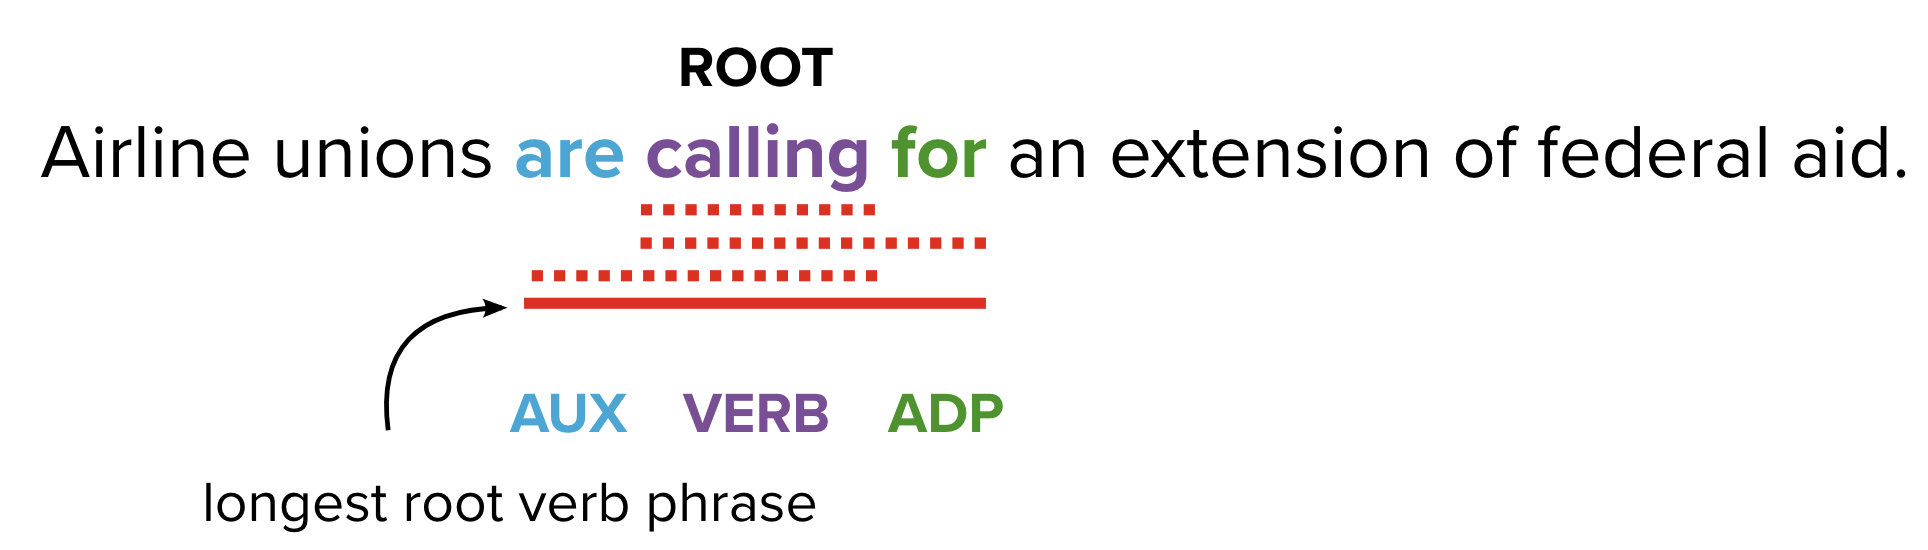
\includegraphics[scale=0.4]{images/verb_phrases.png}
\caption{Verb phrases extracted from an example sentence from article corpora}
\label{verb_phrases}
\end{figure}

% \begin{algorithm}
% \caption{My algorithm}
% \begin{algorithmic}[1]
% \Procedure{MyProcedure}{}
% \State $\textit{stringlen} \gets \text{length of }\textit{string}$
% \State $i \gets \textit{patlen}$
% \If {$i > \textit{stringlen}$} \Return false
% \EndIf
% \State $j \gets \textit{patlen}$
% \If {$\textit{string}(i) = \textit{path}(j)$}
% \State $j \gets j-1$.
% \State $i \gets i-1$.
% \State \textbf{goto} \emph{loop}.
% \State \textbf{close};
% \EndIf
% \State $i \gets i+\max(\textit{delta}_1(\textit{string}(i)),\textit{delta}_2(j))$.
% \State \textbf{goto} \emph{top}.
% \EndProcedure
% \end{algorithmic}
% \end{algorithm}

\subsection{Extracting Noun Phrases}

After the extracting the verb phrases for relations, the same is done for noun phrases in the sentences. As discussed in key decisions in order to capture meaningful relation, the model focuses on extracting subjects and objects as nouns. The most common sentence structure follows the dependency of subject-relation-object in that order. Therefore, for the scope of this project, the focus is directed to these types of semantic relations. First and foremost, for each sentence, the noun phrases are extracted in that sentence which uses chunking and POS-tagging exposed by SpaCy. These return a list of \texttt{Spans}, which are essentially slices of the sentence and contain information such as start, end position are of the phrase (slice) in teh sentence. Additionally, for each sentence all the relevant named entities are also extracted using the Fine-Grained NER model. These entities allowed all types such as 'GPE,' 'PER', 'LOC', 'ORG', 'NORP' etc. except for 'DATE', TIME', 'CARDINAL', 'PERCENT' and 'QUANTITY' \hl{(See Appendix for reference)}. This reason for this was the for each article corpus associated with a topic, the aim was to find information about named entities and how they related to one another. In particular, the model enforces the subject node to be about an entity. Therefore, including entity types such as 'DATE' for instance, can result in unnecessary and irrelevant triples with ('two', 'CARDINAL') as the subject node. This is not to say that any information about 'DATE', 'QUANTITY' etc. is completely ignored. Phrases containing these types of entities often show up object nodes when they are reference to a 'valid' subject named entity. 

\textbf{A base noun phrase, or “NP chunk”, is a noun phrase that does not permit other NPs to be nested within it, so no NP-level coordination, no prepositional phrases, and no relative clauses. copied from spacy doc}

\subsubsection{Subject phrases}

\todonum[inline]{Mad convoluted - rewrite}
In order to obtain the subject phrases, the noun phrases (returned as a list of Spans) are filtered to obtain those that have a starting position less than the starting position of the verb phrase as seen in line 5 in \ref{subject_phrase}. This essentially results in all noun phrases that are at the left of the root verb phrase. Additionally, as mentioned in Section \ref{subject_ents} since the subject node is enforced to be a valid entity, the noun phrases are filtered to obtain candidate subject phrases (\texttt{valid\_ents}) that mention a valid entity from the ones extracted from the sentence. From these candidate subject phrases, we obtain the first occurring (based on position of span) qualifying phrase as the subject phrase (lines 9-10). As seen in \ref{subject_phrase} on line 11, once the first qualifying phrase (i.e. entity) is found, the subject noun phrase is split to obtain the entity (which is the subject)  and the remnant phrase which gets prepended to the verb phrase to form the updated relation phrase. This way the information conveyed by the noun phrase is conserved but the subject nodes are maintained as an entity so a connected knowledge graph can be formed indicating the entity as the subject and showing relationships between these entities and relationships to other object nodes. 

\begin{listing}[H]
\caption{Get subject and relation}
\label{subject_phrase}
\begin{minted}[linenos]{python}
def get_subject_relation(verb_phrase, noun_phrases, ents):
  subject = None
  relation = None
  for n in noun_phrases:
    if n.start < verb_phrase.start:
      valid_ents = [(i,n.text.find(i)) for i in ents if n.text.find(i) != -1]
      if len(valid_ents) == 0:
        continue
      valid_ents.sort(key=lambda tup: tup[1])
      subject = valid_ents[0][0]
      relation = n.text.partition(subject)[2].strip() + ' ' + verb_phrase.text
      break
  return subject, relation
\end{minted}
\end{listing}

\subsubsection{Get object phrase}
The object phrase is also derived from the noun chunks in the sentence but instead of filtering the noun phrases occuring before the root verb phrase, the candidate object phrases obtained by finding all noun phrases (spans) where their starting position in the sentence is after the root verb phrase.

This particular method avoids the stringent dependency of the "subject" and "object" phrases on their actual dependency positions in the grammar, This is because given the nature of news articles, the sentence structure is relatively complex with several different subjects and objects. For the knowledge graph, ultimately, the relations extracted need to focus around different named entities. Relying on the dependency grammar structure to find the subject and object dos not hold as in a given sentence, the structure of the sentence heavily influences the information extracted. This means that more often than not, relevant information about entities is lost due to the entity not necessarily having one of \texttt{"nsubj", "csubj", "nsubjpass",	"csubjpass"} as the dependency. 

\todonum[inline]{Show types of relations extracted with dep parsing and otherwise}
\todonum[inline]{Talk about the object-relation-subject gotcha.}

\subsubsection{Filtering triples}
Once the semantic triples are obtained from the article corpus for each topic, the triples are filtered. After ensuring the that all components of the triple are not null, the triples where the relations/predicates contains words like "said" and "told" in their different forms are filtered. This is done because, often in news articles, direct quotes are made by entities and the relation extraction engine retrieves some poor relations that do not add to the quality of the relations extracted for a particular entity \hl{as seen in Figure} !!!! 

\todonum[inline]{Show some poor relations with said and told}

Once the qualifying semantic triples for each topic are obtained, these are passed to the visualisation engine. An example of the semantic relations extracted for the topics for a given cluster in Business 2021 is shown in \hl{Figure ??}

\chapter{Evaluation}   \label{ch:6:eval}

In this section, the main body of work is evaluated based on objectives defined at the beginning of the project (Section \ref{objectives}) and are detailed as follows:
\begin{enumerate}
    \item Investigate the effect of different pre-processing techniques on semantic clustering and topic modelling.
    \item Investigate the effect of different word embedding models on the quality of clustering.
    \item Investigate the effect of different word embedding models and runtime environments on the performance (in terms of time efficiency).
    \item Evaluate the legibility of the results from the Topic Extraction Engine and Semantic Triple Extraction Engine based on user feedback.
\end{enumerate}

\section{Quantitative evaluation of semantic clustering} \label{s:evaluation_semantic_clustering}

\subsection{Effect of different processing techniques on clustering} \label{s:preprocess_clustering}

In order to cluster the news articles, different pre-processing techniques were applied to the article corpora in the Topic Extraction Engine (See~\Cref{s:procesing_topic_engine}) as a prerequisite for article vector generation for semantic clustering. These techniques included coreference resolution (CR), lemmatisation, stopword removal and named entity removal. The motivation behind this was to gauge the effect of these techniques on the silhouettes scores and incorporate those that the result in the most optimal scores, thereby resulting in improved clustering. \Cref{fig:pre-processing_sil} illustrates how omitting these different pre-processing techniques affects the silhouette score of the semantic clustering obtained for the Year-Category data group: Travel 2021. We can see that not doing any pre-processing (`No pre-processing') on the articles in Travel 2021 results in a poor silhouette score of 0.36 compared to `All', which results in a silhouette score of 0.691 and involves performing coreference resolution, lemmatisation, named entity and stopword removal. A silhouette score near 1 indicates dense, nicely separated clusters, while a score near 0 indicate significant cluster overlap (i.e., distance between them is insignificant). \Cref{fig:pre-processing_sil} shows the general trend that omitting any of these pre-processing techniques deteriorates the quality of clustering, by resulting in poor silhouette scores which indicate overlapping clusters.

\begin{figure}[H]
\centering
  \begin{minipage}[t]{.49\linewidth}
    \centering
    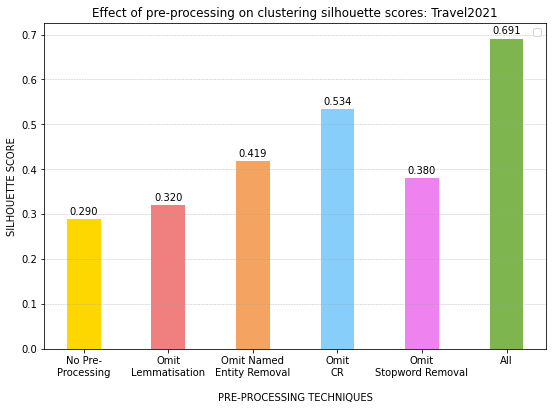
\includegraphics[width=\linewidth]{images/eval/effect_preprocessing.png}
    \caption{-}
    \label{fig:pre-processing_sil}
  \end{minipage}
  \begin{minipage}[t]{.49\textwidth}
    \centering
    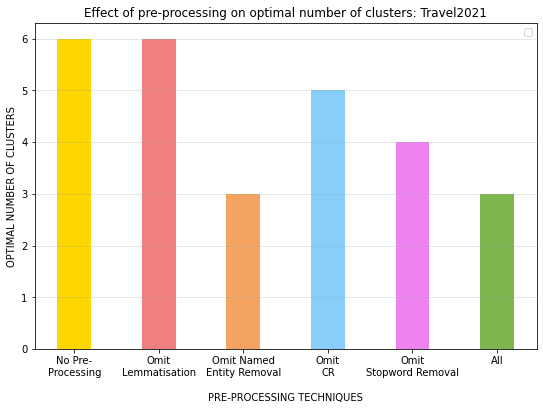
\includegraphics[width=\linewidth]{images/eval/preprocessing_cluster_no.png}
    \caption{-}
     \label{fig:pre-processing_cluster_no}
  \end{minipage}
\end{figure}

Another interesting observation as seen in~\Cref{fig:pre-processing_cluster_no} is how pre-processing affects the optimal number of clusters determined by the Topic Extraction Engine by running the KMeans clustering algorithm with a range of different `k' (See~\Cref{s:optimal_clusters}) and the optimal `k' (number of clusters) as the one that gives the highest silhouette score. Generally, the aim is to get the best silhouette score with the smallest number of clusters. This is because we do not want the Topic Extraction Engine to over-cluster the data by fixating on small differences within the corpus. The semantic clusters are derived for topics to be modelled within them, therefore, we want the engine to achieve a high-level semantic grouping of articles in the form of few, substantially large, distinct clusters. In the example shown in~\Crefrange{fig:pre-processing_sil}{fig:pre-processing_cluster_no}, Travel 2021 was selected as it has a very few number of member articles: 17. Not performing any pre-processing results in 6 clusters for a group of 17 articles. This is excessive as it means each semantic cluster has about 2 or 3 articles. Therefore, the latent topics extracted from these will be modelled on an extremely small corpus of about 2 articles and will most likely be incoherent. For the same data group, performing all the techniques mentioned (i.e., coreference resolution, lemmatisation, named entity and stopword removal), results in a much lower number of clusters: 3. In conclusion, the trend established by \Crefrange{fig:pre-processing_sil}{fig:pre-processing_cluster_no} \hl{is that by performing the pre-processing techniques mentioned , the engine is able to cluster the articles in a Year-Category group in fewer as well as more distinct clusters indicated by the lower optimal number of clusters and higher silhouette scores.}

% \todonum[inline]{Add LDA}

\subsection{Effect of filtering by POS tags on clustering} \label{s:pos_clustering}
% \todonum[inline]{And LDA}
Another key decision made in the Topic Extraction Engine in an attempt to improve the clustering of the input data was to filter the tokens extracted from the articles by their Part-Of-Speech (POS) tags. The decision was made to only use nouns tokens to represent each article. As mentioned earlier, in order to obtain the optimal number of clusters (optimal `k'), the engine performs Kmeans clustering with different values of `k', choosing the one which results in the highest silhouette score. \Crefrange{fig:pos_business2020}{fig:pos_pursuit2021} show the optimal cluster number and silhouette score for the Year-Category data groups: Business2020, Business2020, Politics2021 and Pursuit2021 when allowed POS tags are just `NOUN' and when they are `NOUN', `VERB', `ADJ' and `ADV'. These figures highlight the general trend that having a noun only tokens list to represent the articles for generating article vectors (for semantic clustering) gives a higher silhouette score with a smaller number of clusters. For instance, in~\Cref{fig:pos_business2021}, the silhouette score for noun only tokens list is 0.59 compared to 0.48 when tokens list contains nouns, adjectives, verbs and adverbs, resulting in a 23\% improvement in silhouette score and indicating better clustering for noun-only tokens list. The same is true for \Crefrange{fig:pos_politics2021}{fig:pos_pursuit2021} which show an 8.3\% and 16.3\% improvement respectively for clustering articles based on noun-only article corpus.

\begin{figure}[H]
\centering
  \begin{minipage}[t]{.49\linewidth}
    \centering
    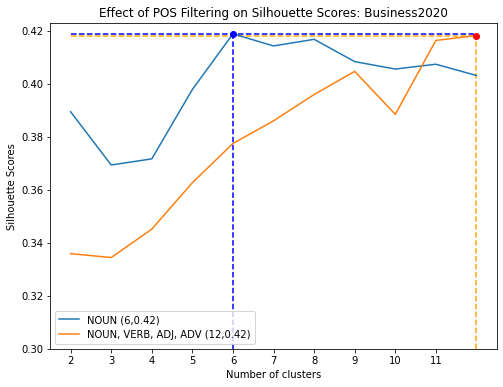
\includegraphics[width=\linewidth]{images/eval/business2020_sil.png}
    \caption{-}
    \label{fig:pos_business2020}
  \end{minipage}
  \begin{minipage}[t]{.49\textwidth}
    \centering
    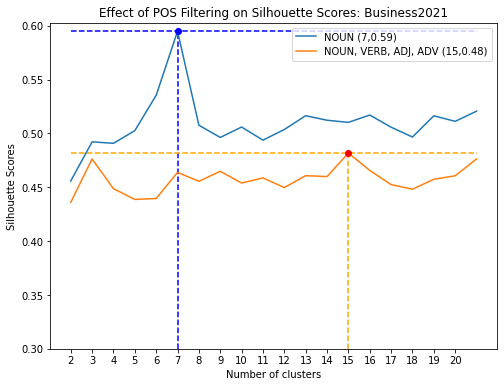
\includegraphics[width=\linewidth]{images/eval/business2021_sil.png}
    \caption{-}
    \label{fig:pos_business2021}
  \end{minipage}
  \begin{minipage}[t]{.49\textwidth}
    \centering
    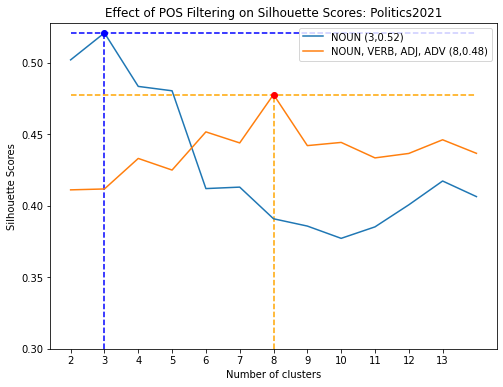
\includegraphics[width=\linewidth]{images/eval/politics2021_sil.png}
    \caption{-}
    \label{fig:pos_politics2021}
  \end{minipage}
  \begin{minipage}[t]{.49\textwidth}
    \centering
    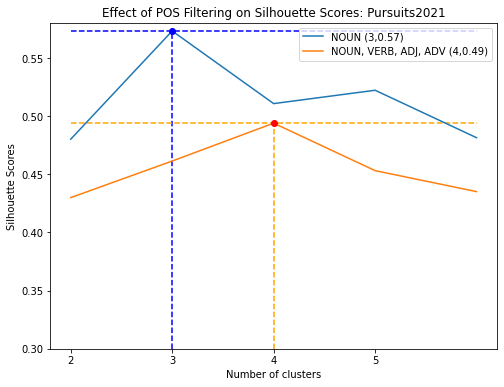
\includegraphics[width=\linewidth]{images/eval/pursuits2021_sil.png}
    \caption{-}
    \label{fig:pos_pursuit2021}
  \end{minipage}
\end{figure}

More evidently, it is important to note that the optimal number of clusters is much lower with a noun-only corpus as seen in the figures above. \Cref{fig:pos_business2020} shows that the silhouette score of 0.42 is achieved with only 6 clusters for noun-only tokens list compared to 12 clusters with nouns, adjectives, verbs and adverbs. For example, \textit{['coronavirus', 'aviation', 'industry', 'border', 'restriction', 'travel, 'quarantine']} is a more concise and general representation of an article as opposed to \textit{['job', 'wipe', 'bad', 'come', 'worker', 'tell', 'worker', 'coronavirus', 'spend', 'lengthy','drastically', 'quarantine']}. Adjectives, adverbs and verbs are not meaningful on their own. Additionally, their generic nature means they are not unique to articles and including them in the \texttt{filtered\_tokens} allows them to equally contribute to their corresponding article vectors as distinctive nouns (e.g., `pandemic') in the corpus, thereby making the article vector less precise. Furthermore, the more tokens used for generating the document vectors, the greater the potential to introduce noise, resulting in high variance among vectors, making the corpus difficult to cluster, and thereby resulting in suboptimal clustering (with more clusters than necessary).

\subsection{Effect of different word embedding techniques on clustering} \label{s:word_embeddings}

\begin{figure}[H]
\centering
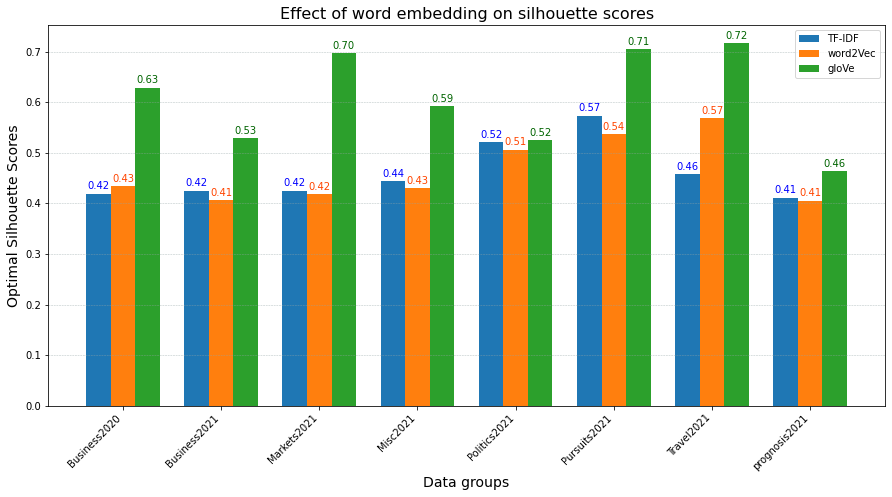
\includegraphics[width=0.7\linewidth]{images/eval/word_embedding.png}
\caption{Effect of using TF-IDF, Word2Vec and GloVe as word embedding model on clustering silhouette scores}
\label{fig:word_embed}
\end{figure}
\vspace{-1em}
As discussed in~\Cref{word_embed_approaches}, in order to cluster the articles, each article's corresponding list of \texttt{filtered\_tokens} is vectorised. \Cref{fig:word_embed}, highlights the effect of the different word embedding techniques, in particular, TF-IDF, Word2Vec and GloVe on the silhouette scores of clusters thereby providing a quantitive measure of how the `goodness' of semantic clustering is influenced by the word embedding approaches. As indicated by the bar chart in Figure \ref{fig:word_embed}, using GloVe to vectorise the articles gives a major improvement in the silhouette scores across all the Year-Category input groups, compared both to TF-IDF and word2Vec.

\begin{table}
\centering
\renewcommand{\arraystretch}{1.05}
\begin{tabularx}{0.7\textwidth}{X X X} 
\multicolumn{3}{c}{GloVe Percentage Improvement} \\
 \hline
 Data group & TF-IDF & Word2Vec \\
 \hline
 Business 2020 & 50.14\% & 45.02\%  \\ 
 Business 2021 & 24.45\% & 30.13\%  \\
 Markets 2021 & 63.91\% & 66.68\% \\
 Misc 2021 & 33.40\% & 37.81\% \\
 Politics 2021 & 0.76\% & 3.71\% \\
 Pursuits 2021 & 23.06\% & 31.41\%  \\ 
 Travel 2021 & 56.58\% & 26.11\% \\
 Prognosis 2021 & 12.72\% & 14.32\% \\ 
 \hline
 Average & 33.13\% & 31.90\% \\ 
\end{tabularx}
\caption{Percentage improvement for silhouette scores when using GloVe over TF-IDF and Word2Vec for all Year-Category data groups}
\label{table:word_embed}
\end{table}

Table \ref{table:word_embed} shows the (percentage) improvement in silhouette scores when using GloVe over TF-TDF and Word2Vec. We see a 33.13\% improvement in clustering (by means of improved silhouette scores) when using GloVe instead of TF-IDF and 31.90\% improvement when compared to word2Vec. Based on these results, it is evident that using GloVe is the optimal approach for word embedding for token vectorisation for semantic clustering. Additionally, we gain confidence in using GloVe as the silhouette scores for the clustering of most input groups are around 0.7 (as seen in~\Cref{fig:word_embed}) which shows evidence of distinct clusters of articles. When clustering news articles, especially articles pertaining to a specific industry within a category, obtaining a perfect clustering with silhouette score of 1 is not realistic, as there is bound to be common underlying themes resulting in some overlap.
% \todonum[inline]{FOR TOPIC MODELLING Do a comparison TABLE for the different sets of allowed postags, Remove adjective noun gives better performance, can show in sil score}

\section{Quantitative evaluation of topic modelling} \label{s:evaluation_topic_extraction}

\subsection{Effect of pre-processing on topic modelling} \label{s:preprocess_topic}

\begin{figure}[H]
  \centering
    \begin{minipage}[t]{.49\linewidth}
      \centering
      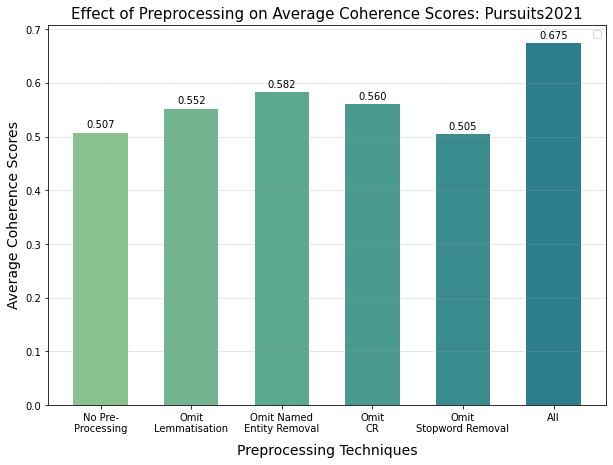
\includegraphics[width=\linewidth]{images/eval/coherence_preprocess.png}
      \caption{-}
      \label{fig:preprocess_topic}
    \end{minipage}
    \begin{minipage}[t]{.49\textwidth}
      \centering
      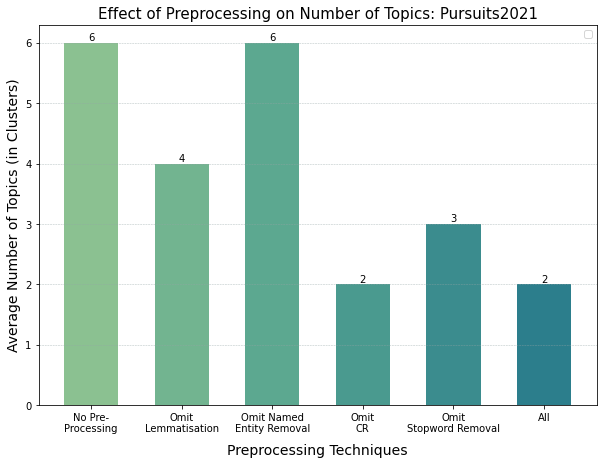
\includegraphics[width=\linewidth]{images/eval/preprocessingTopicNo.png}
      \caption{-}
       \label{fig:pre-processing_topic_no}
    \end{minipage}
  \end{figure}

 Similar to~\Cref{s:preprocess_clustering}, this section also focuses on the effect of pre-processing techniques but on the topics extracted from semantic clusters in Year-Category groups. The topics extracted from each cluster result in a topic coherence score and these are averaged over all clusters in a Year-Category input group to give an average coherence score (for the input group). The coherence score is a useful metric for evaluating the quality of topics extracted as it assesses the degree of semantic similarity between high-scoring terms in a single topic. In similar trends as seen for semantic clustering,~\Crefrange{fig:preprocess_topic}{fig:pre-processing_topic_no} show that applied all the pre-processing techniques (represented by the 'All' bar) results in a significantly higher average coherence score with less number of topics compared to other approaches.  

In the case of omitting coreference resolution, the (average) coherence score falls (to 0.560) as word tokens such as 'it', 'they', 'those' (essentially, unresolved pronouns) do not contribute to the semantic similarity with other high scoring terms in the corpus. Therefore, resolving these pronouns to their respective nouns, means that the frequency of the nouns increases, and they are more likely to contribute to the topics in the corpus. Omitting lemmatisation similarly results in a drop in coherence (and increase in number of topics) as the tokens are not resolved to their base forms affecting the frequency of common words (e.g. tourist and tourists will be treated as different keywords).

As mentioned in~\Cref{data_cleaning}, stopword list contains the default spaCy stopwords (around 326 words), augmented with a custom list of frequently occurring unnecessary words and phrases specific to the input data such as `told', `said' (as news article commonly quote entities, especially people) and `airline', `flight etc. (since news article are specific to the airline industry). The latter are removed as they can be thought of as overarching themes spanning many topics but do not contribute to a distinct topic. The idea is that we do not want the model to fixate on these commonly appearing contextless stopwords and output junk topics, hence why removing them results in better topic coherence (0.775 denoted by the \qs{All} bar) as seen in \ref{fig:preprocess_topic} compared to when they are retained which results in a lower topic coherence of 0.639.

As established prior, named entity removal is done to allow the engine to find distinct topics within a cluster that are not dependent on the named entities. For instance, let's assume that there is a huge overlap between \qs{pilot unions} and \qs{British Airways}. Retaining named entities in the input corpus could result in the model selecting `British Airways' as a topic instead of 'pilot unions'. \Cref{fig:pre-processing_topic_no}, indicates that retaining named entities significantly increases number of topics (6). Some of these topics are `junk', have low coherences scores implied by the lower average coherence score of 0.582 in~\Cref{fig:preprocess_topic}. This makes sense as named entities can be associated with several topics resulting in overlapping clusters, which may be split resulting in more (incoherent) topics. Finally, as expected, omitting all pre-processing results in the lowest average coherence score of 0.401 and highest number of topics (6). 

\subsection{Effect of filtering by POS tags on topic modelling} \label{s:pos_topic}

\begin{figure}
  \centering
    \begin{minipage}[t]{.49\linewidth}
      \centering
      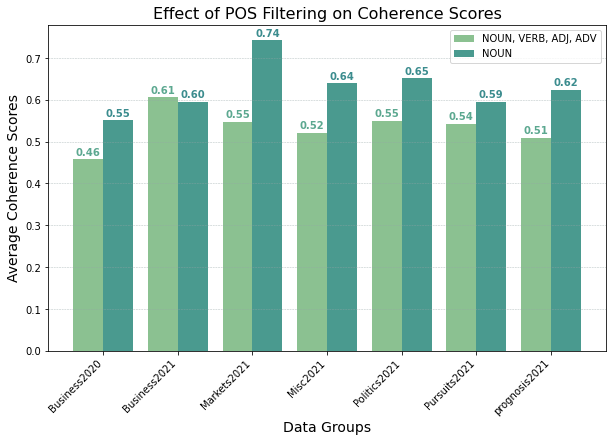
\includegraphics[width=\linewidth]{images/eval/pos_coherence.png}
      \caption{pos}
      \label{fig:pos_topic}
    \end{minipage}
    \begin{minipage}[t]{.49\linewidth}
      \centering
      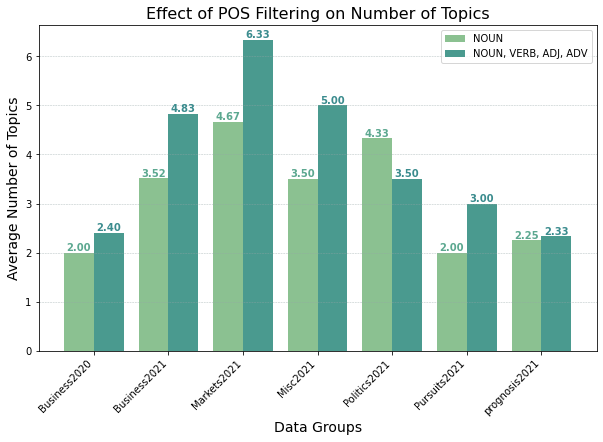
\includegraphics[width=\linewidth]{images/eval/topics_pos.png}
      \caption{-}
       \label{fig:topics_pos}
    \end{minipage}
  \end{figure}

The \texttt{filtered\_tokens} list (for each article) that was used to generate the article vectors for clustering, is passed to the LDA model to extract topics from each of the semantic clusters for a Year-Category group. In order to determine the effect of different allowed POS tags on the quality of topics extracted, the coherence score measure is used. From~\Cref{fig:pos_topic}, it is apparent that the noun only tokens approach to extract tokens performs better than when noun, adjectives, verbs and adverbs are used as the average coherence scores are generally higher for the former approach. Across all the data groups, we see an average coherence score improvement of 18.2\% with the noun only topic extraction approach. This is because, as mentioned in~\Cref{s:pos_clustering}, there are several generic adverbs, adjectives and verbs that occur across articles in high frequency. Including these in the LDA corpus for topic extraction increases the potential for the model to select these as keywords (high-scoring terms) for a topic. This would result in a low semantic similarity among the keywords in a topic, resulting in poor coherence score. The lack of similarity in the filtered tokens articles in LDA corpus would result in the model fitting to the noise, resulting in a higher number of incoherent `junk' topics. This is apparent from \Crefrange{fig:pos_topic}{fig:topics_pos} which show that using `NOUN, VERB, ADJ, ADV' results in lower coherence scores for higher number of topics.


\section{Time Efficiency}

\subsection{Comparing Runtimes in Various Environments}
\vspace{-1ex}

\begin{table}[H] 
\centering
\renewcommand{\arraystretch}{1.05}
\begin{tabularx}{\textwidth}{X X X X} 
 \hline
%  {\hsize=.25\hsize\linewidth=\hsize}Data group & {\hsize=.25\hsize\linewidth=\hsize}CPU & {\hsize=.3\hsize\linewidth=\hsize}Multiprocessing CPU & {\hsize=.2\hsize\linewidth=\hsize}GPU \\
Data group & CPU &  Multiprocessing (CPU) & Tesla T4 GPU \\
 \hline
 Business 2020  & 351.41  & 352.51  & 39.47 \\ 
 Business 2021  & 1713.60 & 1431.80 & 138.47 \\
 Markets 2021   & 839.75  & 1252.64 & 74.18\\
 Misc 2021      & 215.41  & 337.49  & 18.60 \\
 Politics 2021  & 856.42  & 1267.96 & 64.87 \\
 Pursuits 2021  & 178.54  & 377.49  & 15.00 \\ 
 Travel 2021    & 169.52  & 452.80  & 12.92 \\
 Prognosis 2021 & 583.33  & 888.27  & 51.63 \\ 
 \hline
 Total time (s) & 4907.98 & 1920.16 & 414.60 \\ 
 Total time (min) & 81.80  & 32.10 & 6.90\\ 
\end{tabularx}

\caption{Time taken to run the Semantic Analysis Engine pipeline for all data groups(in seconds)}
\label{table:cputime}
\end{table}
\vspace{-2em}
\Cref{table:cputime} shows the different runtimes for the pipeline when running on a CPU, with multiprocessing (on CPU) and GPU (Tesla T4). Ideally, the pipeline is meant to be run on the GPU as it results in significant improvement in computation time, with the whole process of running the pipeline for all the input groups from the dataloader taking only 6.9 minutes in comparison. This is 11.8 times faster than running it on the CPU and 4.6 times faster than running it on the CPU with multiprocessing. The reason for the high computation time for CPU is due to the expensive calls to the AllenNLP models, particularly the Fine-Grained NER, SpanBERT Coreference and RoBERTa Sentiment models (See~\Cref{s:models}), which unlike spaCy, are not built for production use and therefore not optimised for time. However, given that they are state-of-the-art models that achieve high performance for their respective NLP tasks, their use is extremely beneficial to the project. This motivated the use of multiprocessing and designing the engine architecture as a pipeline which takes an input Year-Category data group and outputs the results for the visualisation tool (See \Cref{fig:sys_arch}), to allow for feasible CPU computation. 

Processes are traditionally constrained to just having access to their own process memory, however shared memory permits data structures to be shared between processes. The AllenNLP models in question are significantly large and RAM-intensive and therefore, having multiple copies of the models (one for each process) can result in the machine running out memory. Therefore, it is crucial to store these models in shared memory in order to provide centralised access to all running processes and avoid redundant copies of models for each process. This allowed running the tool on the 8 different data groups simultaneously, resulting in a performance gain in terms of time efficiency as seen in~\Cref{table:cputime}, which shows that using multiprocessing results in 2.55 times lower computational time compared to running with single process CPU. This is because the idle time is significantly reduced by concurrent processes during the expensive calls for coreference resolution, sentiment analysis and NER. 

\subsection{Effect of different word embedding models on GPU runtime}
\vspace{-1ex}
\begin{table}[H]
\centering
\renewcommand{\arraystretch}{1.05}
\begin{tabularx}{0.9\textwidth}{X X X X} 
\multicolumn{4}{c}{GPU runtime (in seconds)} \\
 \hline
 Data group & TF-IDF & Word2Vec & GloVe \\
 \hline
 Business 2020 & 44.67& 33.82& 39.47 \\ 
 Business 2021 & 256.19 & 130.56 & 138.47 \\
 Markets 2021 & 87.30 & 75.00 & 74.18 \\
 Misc 2021 & 16.67 & 17.92 & 18.60 \\
 Politics 2021 & 60.72 & 71.06 & 64.87 \\
 Pursuits 2021 & 15.00 & 14.38 & 15.00 \\ 
 Travel 2021 & 13.06 & 12.85 & 12.92 \\
 Prognosis 2021 & 53.61 & 59.39 & 51.63 \\ 
 \hline
 Total time (s) & 414.98 & 547.92 & 414.60 \\ 
  Total time (min) & 6.92 & 9.12 & 6.90 \\ 
\end{tabularx}
\caption{Time taken to run the pipeline (on GPU) with different word embedding models}
\label{table:word_embed_time}
\end{table}

\vspace{-3ex}
\Cref{table:word_embed} highlights the effect of different word embedding models on the time taken to run the Semantic Analysis Engine pipeline on the Tesla T4 GPU for all data groups. As established in \Cref{s:word_embeddings}, the Topic Extraction Engine uses \texttt{GloVe} as the word embedding model as it gives a significant improvement in the semantic clustering silhouette scores. Furthermore, it also results in more efficient (faster) computation when running the pipeline for all input data with a total runtime of 414.60 seconds, which is 31.15\% lower than using \texttt{Word2Vec}. The difference in runtimes for when using \texttt{TF-IDF} and \texttt{GloVe} is trivial, however, given the 33.13\% improvement (See~\Cref{fig:word_embed}) in silhouette score of \texttt{GloVe} over \texttt{TF-IDF}, \texttt{GloVe} proves to be the best approach in terms of time efficiency and optimal clustering. 

\section{Qualitative User Evaluation} \label{s:user_eval}
In an attempt to gain a greater understanding of the performance of our tool, user testing was conducted with a focus group of 7 people, including members from Deep Search Labs to obtain qualitative evaluation for visualised results from the Topic Extraction Engine and Semantic Triple Extraction Engine.

\begin{figure}[H]
\centering     %%% not \center
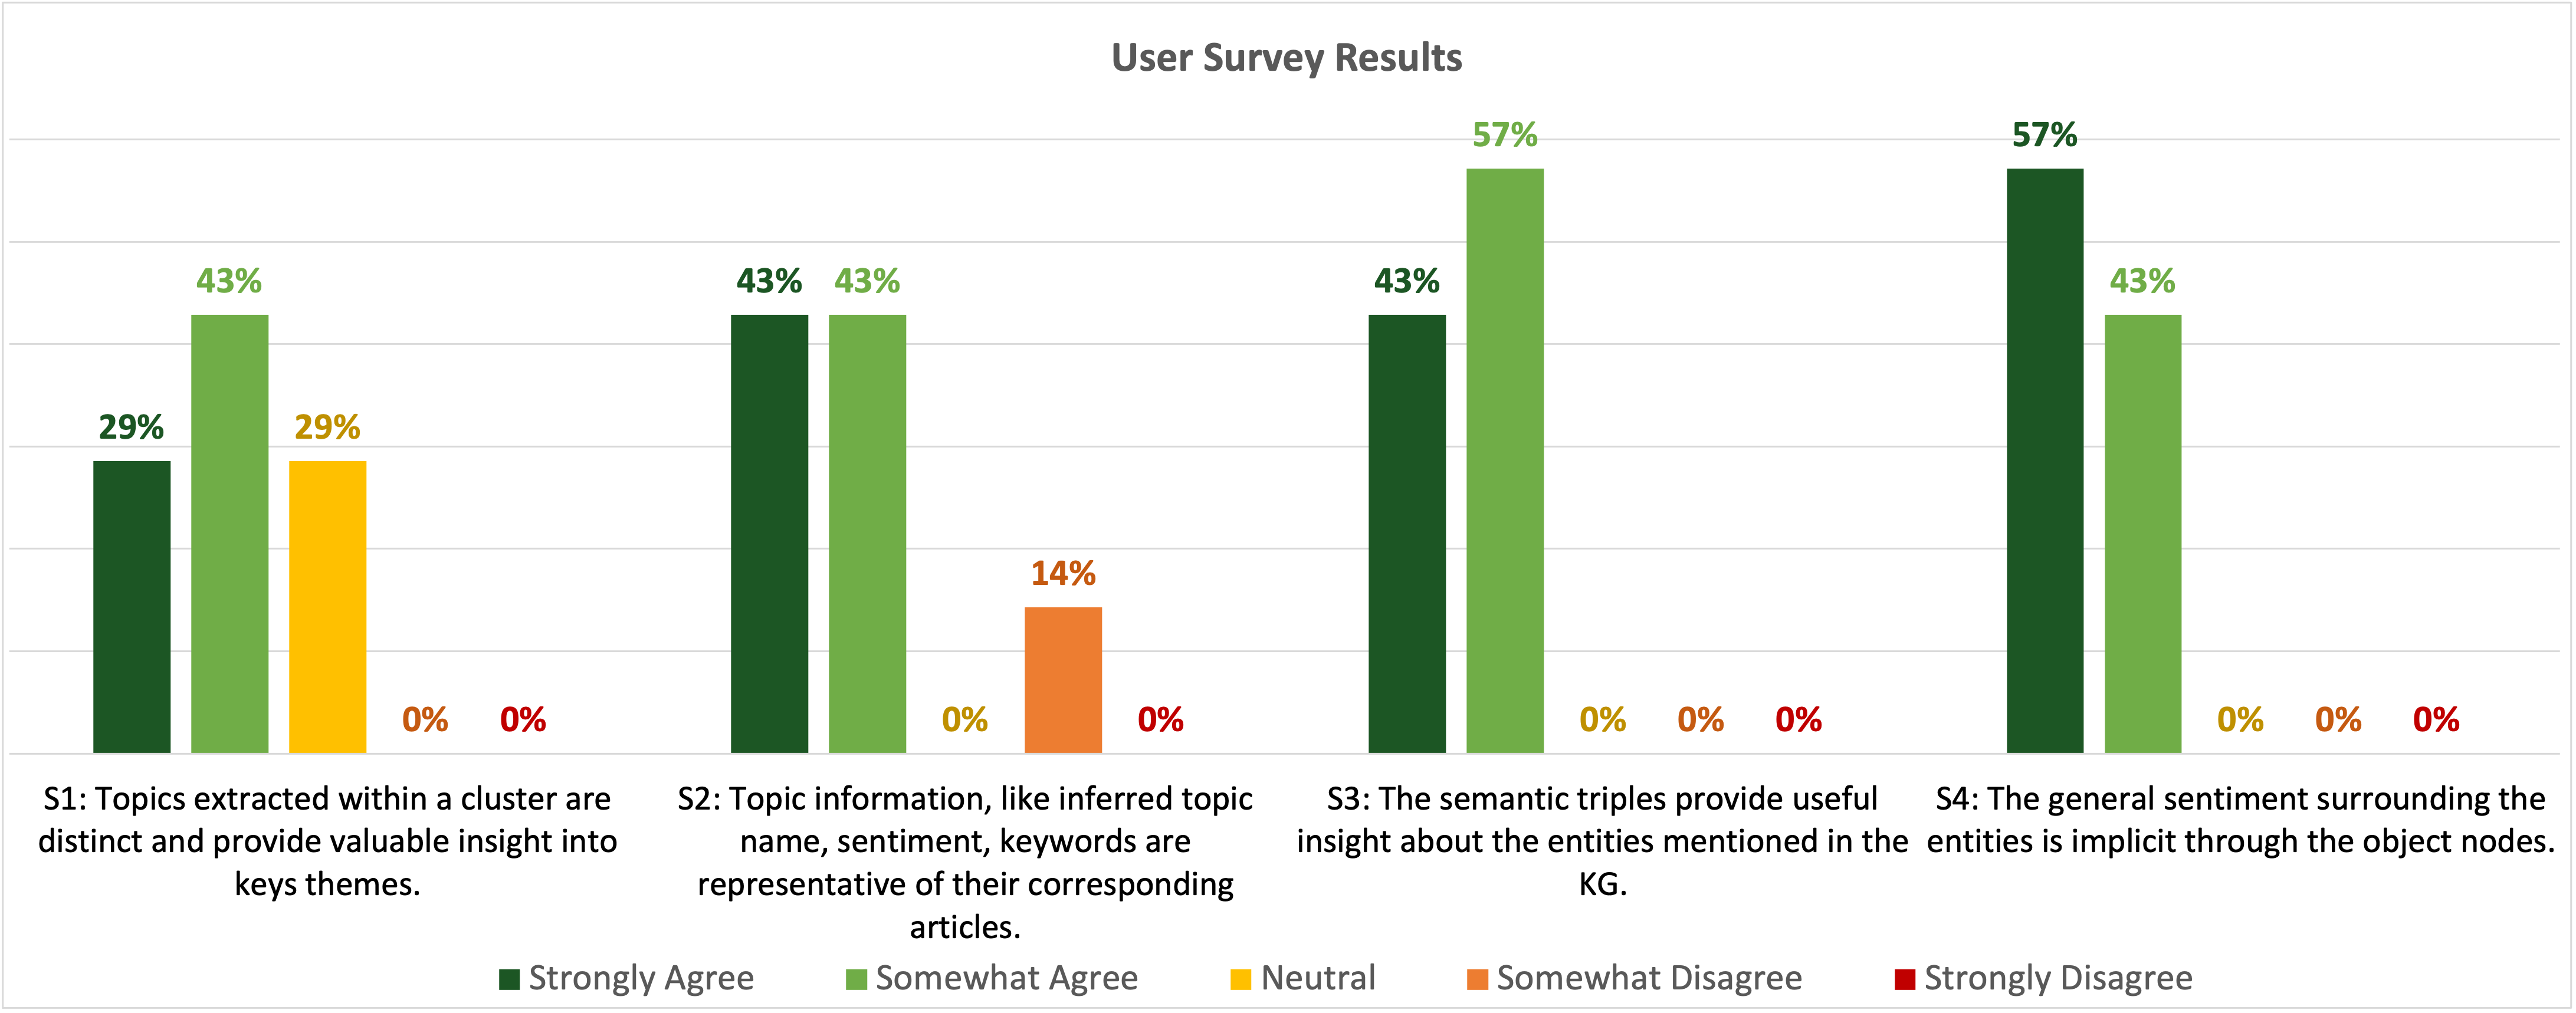
\includegraphics[width=0.95\linewidth]{images/eval/user_eval.png}
\caption{E-}
\label{user_eval}
\end{figure}

The evaluation was conducted in the form of a survey where the users were asked score their agreement for 4 statements based on 5 point scale. In order to ensure uniformity to get a more accurate user perception of the tool, the respondents were asked to focus on the results for the Year-Category input group Travel 2021. \Cref{user_eval} shows the response summary for the 4 statements, where S1 and S2 focus on the cluster-topic graphs for displaying results from Topic Extraction Engine and S3 and S4 focus on the force-directed (knowledge) graph for displaying triples from the Semantic Triple Extraction Engine. 

The responses show that over 72\% of the respondents agree (though only 29\% strongly agree) with statement 1 (S1) that the Topic Extraction Engine is able to extract fairly distinct, coherent latent topics from the semantic clusters, with the other 29\% remaining indifferent. For S2, while 86\% respondents agree that the articles within the topic make sense based on the topic information, 14\% (1 of 7) disagree. This is understandable, because as identified in~\Cref{limitation_topics}, assigning an article a single dominant topic may not always be intuitive. The responses for S3 and S4 were overwhelming positive, with a 100\% agreement for both statements verifying that the semantic triples in the graph provide useful insight about key entities (the relevance of entities depicted by the size of their nodes) and the general sentiment associated with these entities (depicted via green-red colour scheme for positive and negative sentiment respectively). Comparing the agreements responses for S1-S2 with S3-S4, we can infer the qualitative user evaluation gives greater confidence in the Semantic Triple Extraction Engine compared to Topic Extraction Engine, although both were received as there were no strong disagreements with any of the statements (which generalise some of the objectives of the engines). 

\chapter{Conclusion}

\section{Summary of achievement}

The aim of this project was to provide a distilled and coherent representation of the news in a particular industry, to provide valuable insight into the pertinent themes, events and entities in a particular category of news for a set period of time. Our work has succeeded in doing so by developing a tool that provides cohesive semantic analysis of news by grouping articles in a specific category (such as Travel, Business, Markets, etc.) into semantic clusters, on which latent topics are modelled, using LDA, to summarise the key themes in these semantic clusters (See~\Cref{ch:4:topic}). 
For topic extraction, usually one of either cluster analysis or topic modelling is performed on the input data (news articles), however, by combining these methods we are able to provide a high-level semantic grouping through clustering as well as a finer-grained grouping through topic models, improving the coherence of these the extracted latent topics.
 Using POS filtering, stopword removal, lemmatisation and TF-IDF to pre-process the LDA corpus allows for distinct topics with minimal overlap in the semantic clusters. Additionally, our tool performs semantic triple extraction for each topic in a semantic cluster to obtain a minimal representation of the information provided by articles (associated with the topic) such as the `key entities', their relationships to events and other entities as well as the sentiment of the news surrounding them (\Cref{ch:5:triple}).  

Based on both quantitative empirical results (such as silhouette and coherence scores) as well as qualitative user feedback, the final product gives confidence in the extraction relevant information though topics and triples and displays these results through graphs generated by visualisation tool in the end-to-end semantic analysis engine (See \Cref{fig:sys_arch}). By carrying out extensive research into related works for similar problems, as well as a thorough investigation and evaluative to optimise the different components of the semantic analysis engine in terms of quality of results and time efficiency, we were able to design a novel system which combines several semantic analysis techniques in order to develop a user-friendly, end-to-end pipeline for visualising the news automatically.


% The product successfully met the initial four goals to

% textual entailment to measure
% agreement between articles from different sources.

% Key learnings were very broad, ranging from building scrapers to concurrently collect data from different news
% sources, to conducting complex NER and SRL analysis, to developing user functionality on top of a large network of
% nodes in a force-directed graph.
\section{Wider applications}
The current solution for semantic analysis of news proposed in this project focuses on a single industry, i.e., airline. A wider application for this project could involve using the proposed tool across different industries combining to see how the news across industries affect each other and what common themes or topics, if any, can be extrapolated from the semantic analysis. This could be useful not only for the average consumer but also relevant from a business intelligence standpoint where companies can see, for example, market trends across industries such as airline, energy etc. or travel trends in hotel management and airline industry, getting an insight into how they are affected by each other.

Additionally, collecting more data across different years would be useful as it would allow more substantial temporal semantic analysis of the news, where the user can infer how the topics and content of the news (through triples) changes through different periods of time for new articles associated with a particular industry. 



\section{Future Work}

\begin{enumerate}
    % \item Topic Bert for modelling topics:
    \item \textbf{Sentence relevance for article summarisation:} The current approach for generating the semantic clusters and topics uses the `article intros' rather than the entire article (as they introduce a lot of redundancy). The `intros' consist of the first 8 sentences of the article as the introductions of the articles generally provide a good summary whilst retaining sufficient context. An alternative approach to the `article intros' involves obtaining the extractive text summary of the articles by selecting the most relevant sentences in the corpus through sentence ranking algorithms~\cite{jevzek2008automatic}~\cite{madhuri2019extractive}. 
    
    \item \textbf{Linking to existing Knowledge Base for Disambiguation and Data Augmentation:} The current approach simply relies on the entities extracted from processing raw text from the articles to generate the knowledge graph (of semantic triples). This has the potential of introducing redundancy as the aliases of named entities (e.g. BA and British Airways) do not get resolved to the same entity. A beneficial improvement for the future would be to use named entity linking (NEL)\cite{retrospective_kg} and store the semantic triples in an RDF triplestore where the `subject entity' is represented with a unique International Resource Identifier (IRI) \cite{internationalized}. This allows for Named Entity Disambiguation (See~\Cref{ned}) by removing the dependency of subject nodes on the aliases of named entities. 
    
    \item \textbf{Experiment with ELMo embeddings for document vectorisation.}  The challenges with approaches such as Word2Vec and GloVe word embeddings are that they provide a single context-independent representation for a word and struggle with ``out-of-vocabulary (OOV) words"~\cite{elmo_word_rep}, i.e., words that were never encountered prior will often be represented as a random vector which is not ideal. A potential improvemnt over this would be to use ELMo to allow context-dependant word embeddings (See \Cref{elmo}).
    
\end{enumerate}

\newpage
\renewcommand{\thepage}{}

\appendix
% \listoffigures
% \listoftables
\chapter{POS Tag Definitions}

\begin{table}[H]
    \centering
    \renewcommand{\arraystretch}{1.25}
    \begin{tabularx}{\textwidth}{|>{\hsize=.5\hsize\linewidth=\hsize}X|>{\hsize=1.0\hsize\linewidth=\hsize}X|>{\hsize=1.5\hsize\linewidth=\hsize}X|} 
     \hline
      \textbf{POS Tag} & \textbf{Meaning} & \textbf{Examples} \\
     \hline
        ADJ & adjective & big, pink, first  \\
        \hline
        ADP & adposition & in, to, during \\
        \hline
        ADV & adverb & very, well, tomorrow \\
        \hline
        AUX & auxiliary verb & has (done), is (doing), will (do) \\
        \hline
        CONJ & coordinating conjunction & and, or, but \\
        \hline
        DET & determiner &  a, an, the \\
        \hline
        INTJ & interjection &  ouch, bravo, hello \\
        \hline
        NOUN & noun & tree, air, beauty \\
        \hline
        NUM & numeral &  seventy-seven, 12, IV \\
        \hline
        PART & particle & 's, not \\
        \hline
        PRON & pronoun & you, he, she \\
        \hline
        PROPN & proper noun & Mary, Anji, London \\
        \hline
        PUNCT & punctuation & . ! ? \\
        \hline
        SCONJ & subordinating conjunction & if, while, that \\
        \hline
        SYM & symbol & \$, \%, : \\
        \hline
        VERB & verb & jump, run, dance \\
        \hline
        X & other & scsd, aosa, oooqas \\
    \hline
    \end{tabularx}
    \caption{Universal POS tag set comprising core part-of-speech categories~\cite{universal_pos_tags}}
    \label{appendix:pos}
    \end{table}
    
% \section{Coocc} \label{coocc}


\chapter{Dependency Set Labels}

\vspace{-1em}
\begin{table}[H]
    \centering
    \renewcommand{\arraystretch}{1.0}
    \begin{tabularx}{0.8\textwidth}{|>{\hsize=.3\hsize\linewidth=\hsize}X|>{\hsize=0.7\hsize\linewidth=\hsize}X|} 
     \hline
      \textbf{Dependency Tag} & \textbf{Meaning} \\
     \hline
        acl & clausal modifier of noun (adjectival clause) \\
        \hline
        advmod & adverbial modifier \\
        \hline
        amod & adjectival modifier \\
        \hline
        appos & appositional modifier \\
        \hline
        aux & auxiliary \\
        \hline
        case & case marking \\
        \hline
        cc & coordinating conjunction \\
        \hline
        ccomp & clausal complement \\
        \hline
        clf & classifier \\
        \hline
        compound & compound \\
        \hline
        conj & conjunct \\
        \hline
        cop & copula \\
        \hline
        csubj & clausal subject \\
        \hline
        dep & unspecified dependency \\
        \hline
        discourse & discourse element \\
        \hline
        dislocated & dislocated elements \\
        \hline
        expl & expletive \\
        \hline
        fixed & fixed multiword expression \\
        \hline
        iobj & indirect object \\
        \hline
        nmod & nominal modifier \\
        \hline
        nsubj & nominal subject \\
        \hline
        nummod & numeric modifier \\
        \hline
        obj & object \\
        \hline
        obl & oblique nominal \\
        \hline
        punct & punctuation \\
        \hline
        reparandum & overridden disfluency \\
        \hline
        root & root \\
        \hline
        vocative & vocative \\
        \hline
        xcomp & open clausal complement \\
    \hline
    \end{tabularx}
    \caption{Universal Dependency Tag set~\cite{universal_deps}}
    \label{appendix:deps}
    \end{table}
\chapter{\vspace{-3px}NER Semantic Types}

\vspace{-3em}
\begin{table}[H]
    \centering
    \renewcommand{\arraystretch}{1.2}
    \begin{tabularx}{0.8\textwidth}{|>{\hsize=.3\hsize\linewidth=\hsize}X|>{\hsize=0.7\hsize\linewidth=\hsize}X|} 
     \hline
      \textbf{Dependency Tag} & \textbf{Meaning} \\
     \hline
        CARDINAL &  \\
        \hline
        DATE &  \\
        \hline
        FAC &  \\
        \hline
        GPE &  \\
        \hline
        LAW &  \\
        \hline
        LOC &  \\
        \hline
        MISC &  \\
        \hline
        MONEY & \\
        \hline
        NORP &  \\
        \hline
        ORG &  \\
        \hline
        PERCENT &  \\
        \hline
        PERSON &  \\
        \hline
        QUANTITY &  \\
        \hline
        TIME &  \\
    \hline
    \end{tabularx}
    \caption{Named Entity Types extracted by Fine-Grained NER~\cite{lample}}
    \label{appendix:semantic_types}
    \end{table}

    
    \todonum[inline]{Find all semantic types}



\bibliographystyle{IEEEtran}
\bibliography{IEEEabrv,references}

\end{document}

% Semantic Analysis of News Corpora 
% - Topic Modelling
% - Semantic Relation Extraction
% - Visualising Tool


% Layout:

% - Titlepage + Abstract + Dedications: 3 pages
% - Intro ~ 1-3 pages
% - Background~ 17-18 pages
% - Ethical considerations ~ 1 page
% - Project Structure (briefly describe each component) ~ 3-4 pages
%     - Dataset
%     - System Design 
%     - Models
% (incl. eval  ~30)
% - Processing Data ~ 
% - Semantic Clustering
% - Topic Modelling/Extraction
% - Relation Extraction
% - Visualisation
% (either separate evaluation or in each section)

% - Conclusion + Future work ~ 2 pages